\documentclass[12pt,a4paper,openright]{book}

\usepackage[left=3.5cm,top=2.5cm,right=2.5cm,bottom=2.5cm]{geometry} %margins
\usepackage{amsthm} % theorem environment
\usepackage{amsmath} % math
\usepackage{amssymb} % symbols
\usepackage{graphics} % for including figures
\usepackage{graphicx} % for including figures
\usepackage{setspace} % for doublespacing singlespacing etc.
\usepackage{datetime} % to write the date in the desired format
\usepackage[title, titletoc]{appendix}
\usepackage{subfigure}
\usepackage{algorithm}
%\usepackage{algorithmic}
\usepackage{longtable}
\usepackage{bm}
\usepackage{verbatim}
\usepackage{algorithmicx}
\usepackage{algpseudocode}
\usepackage{float}
\usepackage{listings}
\usepackage{framed}
\usepackage{multirow}
\usepackage[square, comma, sort&compress]{natbib}
\usepackage{hyperref}
\usepackage{fixltx2e}
\usepackage{url}
\usepackage{pdfpages}
\usepackage{caption}
\usepackage{subcaption}
%\usepackage{hyperref}
%\usepackage{afterpage}
\usepackage{fancyhdr}

\theoremstyle{definition}
\newtheorem{example}{Example}
\newtheorem{definition}{Definition}
\newtheorem{proposition}{Proposition}
\newcommand{\todo}[1]{\textcolor{red}{\textbf{TODO:} #1}}
\graphicspath{{img/}}

\pagestyle{myheadings} 

%\setlength{\LTpre}{0pt}
\setlength{\LTpost}{-40pt}
\setlength{\LTcapwidth}{\textwidth}
% % % % % % % % % % % % % % % % %

%all this for generating title and certificate
\newdateformat{monthyear}{\monthname[\THEMONTH], \THEYEAR}
\def\title{GloDETC : Global Document Embeddings for Multi-label Text Classification}
\def\subtitle{}
\def\author{Nitish Gupta}
\def\rollno{10327461}
\def\degree{B.Tech. - M.Tech. (Dual Degree)}
\def\department{Department of Electrical Engineering}
\def\shortdepartment{EE}
\def\institute{Indian Institute of Technology Kanpur}
\def\shortinstitute{I.I.T. Kanpur}
\def\longinstitute{Indian Institute of Technology, Kanpur}
\def\advisormain{Prof. Harish Karnick}
\def\advisorsec{Prof. Rajesh M. Hegde}
\def\advisormaindepartment{Department of Computer Science and Engineering}
\def\advisorsecdepartment{Department of Electrical Engineering}
\def\instituteaddress{Kanpur-208016}

% % % % % % % % % % % % % % % % % 

\hypersetup{
	bookmarks=true,
	bookmarksopen=true,
	bookmarksopenlevel=0,
	bookmarksnumbered=true,
	hypertexnames=false,
	colorlinks=true,
	linkcolor={black},
	citecolor={black},
	urlcolor={black},
	breaklinks=true,
	pdfauthor={\author},
	pdftitle={\title}
}


\begin{document}
	\frontmatter
	\thispagestyle{empty}
	\begin{titlepage}

\pagestyle{empty}
\begin{center}
	\huge{\textbf{\title}}\\
\end{center}

\begin{center}
 \large{\subtitle}
\end{center}


\vspace{0.5in}
\begin{center}
	\large\textit{A Thesis Submitted \\ in Partial Fulfilment of the Requirements \\ for the Degree of}\\
	\vspace{0.2in}
	\large\textbf{\degree}\\

%  \textit{by}\\
\end{center}
\vspace{0.5in}
\begin{center}
	\Large\textit{by}\\
	\Large\bf{\author}\\
	\Large{Roll No. : \rollno}\\
	\vspace{0.35in}
\end{center}

\vspace{0.5in}
\begin{center}
	\Large\textit{under the guidance of}\\
	\Large\bf{\advisormain}\\
	\Large\bf{\advisorsec}\\
	\vspace{0.25in}
\end{center}

\vfill
\begin{center}
\begin{figure}[htbp]
	\centering
	
\includegraphics[width=3cm]{figs/iitkblue.jpg}
\end{figure}

\vspace{0.2in}
\large{\department}\\
\vspace{0.1in}
\large{\institute} \\ 
\vspace{0.03in}
\Large{\monthyear\today}

\end{center}



%\begin{center}
%{\LARGE {\bf \title}} 
%\vfill
%\vspace{0.5in}
% \large\textit{A Thesis Submitted \\ in Partial Fulfillment of the Requirements \\ for the Degree of}\\
% \vspace{0.2in}
% \large\textbf{\degree}\\
% \vspace{0.1in}
%  \textit{by}\\
%\vfill
%%{\em by}\\
%\vspace{12pt}
%{\large \author \vspace{10pt} \\ \rollno } \\
%\vspace{20pt}
%\begin{center}
%
\includegraphics[width=0.25\textwidth]{iitkblue}
%\end{center}
%{\em to the}\\
%\vspace{24pt}
%{\bf \department} \\
%\vspace{12pt}
%{\Large \institute}\\
%\vspace{12pt}
%{\bf \monthyear\today}
%
%
%\end{center}

\end{titlepage}

	
	\newpage
	\thispagestyle{empty}
	\mbox{}

	
	\thispagestyle{empty}
 	%\vspace*{1.0in}
\begin{center}
\begin{large}
{\bf CERTIFICATE}
\end{large}
\end{center}
\vskip 2cm
It is certified that the work contained in this thesis entitled ``{{\textit{\title}}}'',\\ by {{\textit{\author (Roll No. \rollno)}}}, has been carried out under my \\supervision and that this work has not been submitted elsewhere for a degree.
\vskip 1in
\begin{flushleft}
		\hspace*{5.8cm}{\hrulefill}\\
		\hspace*{5.8cm}(\advisormain)\\
		\hspace*{5.8cm}\advisormaindepartment,\\ 
		\hspace*{5.8cm}\institute\\
		\hspace*{5.8cm}\instituteaddress
\end{flushleft}
\monthyear \today % not to be used.
        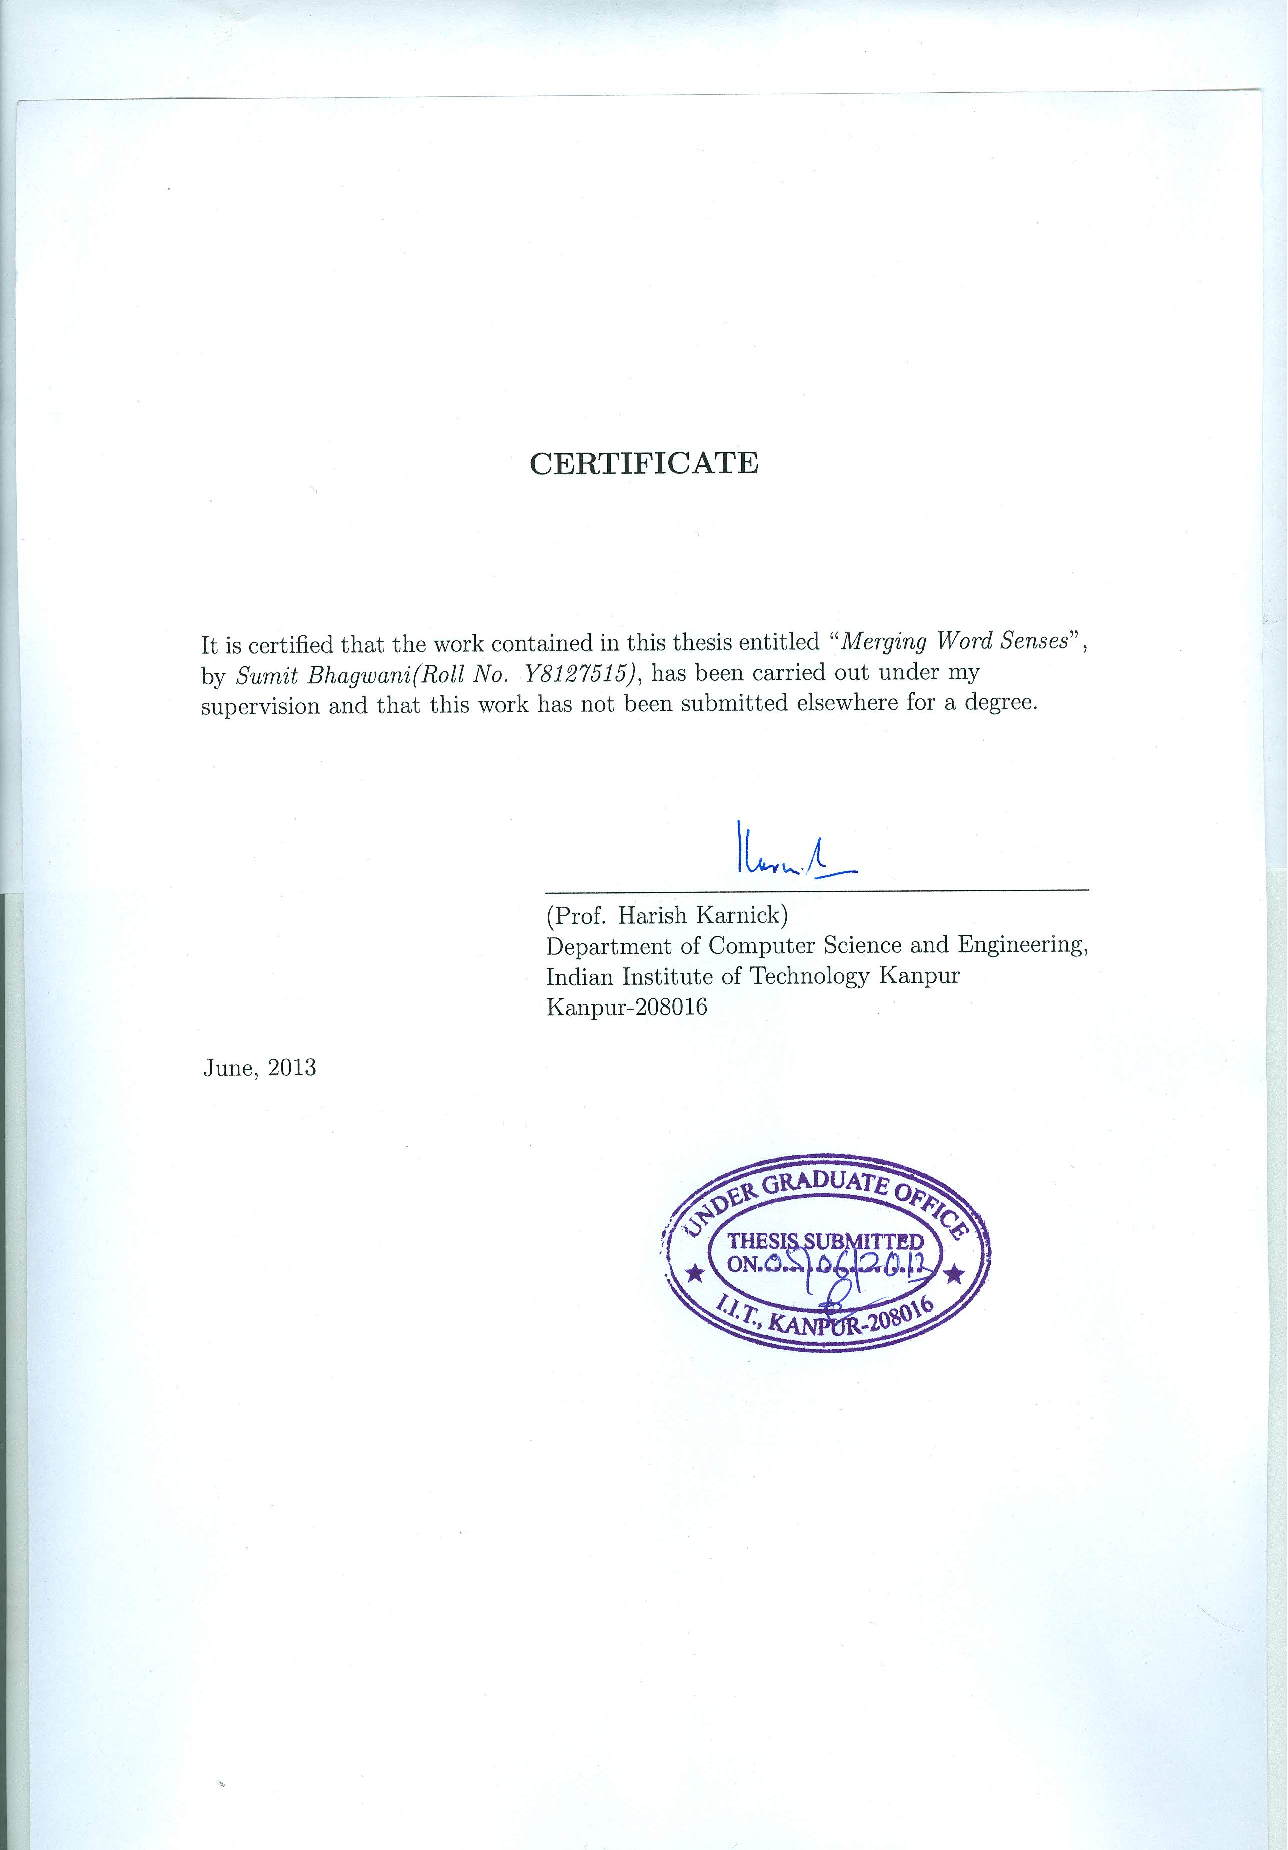
\includepdf{sumitbCertificate.pdf}
	%\pagestyle{myheadings} % not be used I think
	\pagenumbering{roman} 
	\pagestyle{plain}
	
	\newpage
	\thispagestyle{empty}
	\mbox{}

	\setcounter{page}{1} 
	%\setcounter{page}{2}
	\addcontentsline{toc}{chapter}{Abstract}
	
	\onehalfspace
	\begin{center}
\huge{\textbf{Abstract}}
\end{center}

% Multi-label Document Categorization, the task of automatically assigning a text document into one or more categories is a crucial step in knowledge management and has various real-world applications such as categorizing news articles, tagging Web pages, maintaining medical patient records and organizing digital libraries among many others. 
% Statistical Machine Learning approaches to document categorization have focused on multi-label learning algorithms such as Support Vector Machines, k-Nearest Neighbors, Logistic Regression, Neural Networks, Naive Bayes, Generative Probabilistic Models etc. while the input to such algorithms i.e. the vector representation for documents has traditionally been used as the bag-of-words representation model. 
% %The input to such algorithms i.e. the vector representation for documents has traditionally been used as the bag-of-words representation model due to its simplicity and ability to capture the topical content of the documents.
% Though the usage of simple bag-of-words document representation gives surprisingly accurate results, it suffers from sparsity, high-dimensionality and lack of similarity measures along with various drawbacks such as the inability to preserve word ordering and contextual information in which the words occur in the documents. Encoding contextual information about words in documents is crucial to capture the correct semantic content of the highly complex and ambiguous human language.  \hfill \break

% Our work is focused on learning continuous distributed vector representations for documents by embedding all the documents in the same low-dimensional space such that documents that are similar in their semantic content have similar vector representations. To tackle the issues in bag-of-words representation model, we present an unsupervised neural network model that, given a word in a document, uses the document representation along with the contextual information in which the word occurs, to predict it and learn document representations along with learning distributed word vectors. 
% %By learning low-rank distributed representations and incorporating contextual information in which the words occur in the documents we try to overcome the drawbacks posed by the bag-of-words representations. 
% We use a modified version of the logistic regression algorithm to learn similar distributed representations for categories to perform the document categorization task. As we embed documents, categories and words in the same low-dimensional space, estimating similarity between them is as simple as taking a dot-product between the vectors of the entities. We show that the representations learned using our model give state-of-the-art results in the document categorization task on standard \emph{Reuters-21578} and Wikipedia datasets and also show promising results in imputing missing categories in existing articles on Wikipedia against the bag-of-words representations.
Multi-label Document Categorization, the task of automatically assigning a text document into one or more categories has various real-world applications such as categorizing news articles, tagging Web pages, maintaining medical patient records and organizing digital libraries among many others. Statistical Machine Learning approaches to document categorization have focused on multi-label learning algorithms such as Support Vector Machines, k-Nearest Neighbors, Logistic Regression, Neural Networks, Naive Bayes, Generative Probabilistic Models etc. while the input to such algorithms i.e. the vector representation for documents has traditionally been used as the bag-of-words model. Though the usage of simple bag-of-words representation gives surprisingly accurate results, it suffers from sparsity, high-dimensionality, lack of similarity measures along with other drawbacks such as the inability to encode word ordering and contextual information in which the words occur. Encoding contextual information about words in documents is crucial to capture the correct semantic content of the highly complex and ambiguous human language.  \hfill \break

Our work is focused on learning continuous distributed vector representations for documents by embedding all the documents in the same low-dimensional space such that documents that are similar in their semantic content have similar vector representations. To tackle the issues in bag-of-words representation model, we present an unsupervised neural network model that uses the document vector to predict words in the document along with using the contextual information in which the word occurs and jointly learns distributed document and word representations. We use a modified version of the logistic regression algorithm to learn similar distributed representations for categories to perform the document categorization task. We show that the representations learned using our model give state-of-the-art results in the document categorization task on the standard \emph{Reuters-21578} and Wikipedia datasets and also show the effectiveness of our model in imputing missing categories in existing articles on Wikipedia against the bag-of-words representations. As we embed categories and words in the same low-dimensional space we can also estimate similarities between them which is not directly observed in the data. We qualitatively demonstrate that the learned representations are also able to capture the semantic dependencies between categories and words. 
	
	\newpage
	\thispagestyle{empty}
	\mbox{}

	\setcounter{page}{2} 
	
\vspace*{\fill}

\begin{center}
%{\it Dedicated to my parents and my brother}\\
{\it Dedicated to}\\
{\it My Family}
\end{center}

\vspace*{\fill}

	
	\newpage
	\thispagestyle{empty}
	\mbox{}

	\setcounter{page}{3} 
	\begin{center}
	{\huge{\textbf{Acknowledgement}}}
\end{center}
I wouldn't like to express my sincere gratitude towards my thesis supervisor, {\advisormain}, for his constant support and encouragement. I am grateful for his patient guidance and advice in giving a proper direction to my efforts. I am also grateful to {\advisorsec} for giving me the freedom to work on a topic of my liking.

\paragraph*{}
Last, but not the least, I would like to thank my parents and brother for their love and encouragement. Without their support and patience this work would not have been possible. 

\vskip 4mm
\begin{flushright}
\textit{\textbf{\author}}
\end{flushright}






	\newpage
	\thispagestyle{empty}
	\mbox{}

	\setcounter{page}{4} 
	
        \setcounter{secnumdepth}{3}
	\doublespacing
	\setcounter{tocdepth}{3}
	\tableofcontents
	
	\listoftables
	\addcontentsline{toc}{chapter}{List of Tables}
	
	\listoffigures
	\addcontentsline{toc}{chapter}{List of Figures}
	
	\listofalgorithms
	\addcontentsline{toc}{chapter}{List of Algorithms} 
		
	\newpage
	\thispagestyle{empty}
	\mbox{}
 
	\mainmatter
	\doublespacing
	\pagenumbering{arabic}
	\pagestyle{myheadings}
	
	%\pagestyle{fancy}
	%\fancyhead[LO,RE]{}
	
	%\chapter{Introduction}
\label{chapter:introduction}

\todo{ Section 2 : Problem Statement. Formally with document vectors $x_{d_{i}}$ and task of finding appropriate label vector $l_{d_{i}}$ Section. Along with table as in http://lpis.csd.auth.gr/publications/tsoumakas-ijdwm.pdf 3 : Contribution Section 4 : Organization of thesis}

Text documents usually belong to more than one conceptual class. For example, a document on music piracy can be simultaneously classified into \emph{Arts/Music}, \emph{Internet/Security}, \emph{Laws/Cyber}.     Multi-Label Document Categorization \emph{(also known as Text Categorization or Classification)} is the task of assigning a text document to one or more pre-defined categories to describe the semantic content of a document and provide a conceptual view of the document collection.
With the growth of online information, Document Categorization has found its use in many important real world applications ranging from document organization to information retrieval. It can be used to organize news stories by categories (topics), classify academic papers by the technical domains and sub-domains they belong to, cluster documents based on their semantic content for easy retrieval and recommendation etc.
With the advent of crowd-sourced databases such as Wikipedia\footnote{www.wikipedia.org} which contains over $4$ million documents that are manually categorized from a category set containing over $500$ thousand categories, automatic document categorization is utmost necessary and useful to assign categories to new articles that are added on a daily basis and also assign missing categories to older documents.

The task of multi-label classification belongs to a general family of supervised learning where the training instances along with the labels they belong to are used to learn a multi-label classifier that assigns appropriate labels to new test instances. 
Another supervised learning task that is very relevant to multi-label classification is that of \emph{ranking}. In the ranking task, the learning algorithm learns a ranking function from the training examples that ranks the set of labels for a new instance such that the more relevant labels are the topmost in the ranked list. 
To generate the proper output of the multi-label classifier, i.e. the set of relevant labels for the test instance, post-processing of the ranked list of categories is required.

Supervised machine learning techniques that learn classifiers to perform the document categorization task can be broken down into two main components, namely, text representation and learning algorithm. 
Text representation involves converting the documents, that are usually strings of characters, into numerical vectors that are suitable inputs to the learning algorithm while the learning algorithm uses pairs of labeled input text representations and the categories it belongs to, to learn a model so as to assign relevant categories to new documents. \todo{ADD COMPLETE SYTEM FIGURE.}

Over the years, documents have been represented as a \emph{bag-of-words} feature vector, which contains information about the presence and absence of words in the document. Given a corpus of documents, each document $d_{i}$ in the corpus is represented as a vector $v_{d_{i}} \in \mathbb{R}^{|V|}$ whose size is equal to the size of the vocabulary. Each element in the vector belongs to $\{0, 1\}$ and denotes whether the particular word is present in the document or not. Though bag-of-words document representation has been widely used for document categorization due to its simplicity, efficiency and ability to capture topical content of the documents necessary for categorization, it suffers from various drawbacks. Bag-of-words representation ignores word ordering and the context in which the words appear in the document, that is vital for encoding the semantic content of text. It also lacks in the ability to encode the semantic similarity between words and documents to estimate distances between them. Disadvantages of such sought have necessitated the need for a more robust and efficient document representation model.
%In the section below we describe the drawbacks of the bag-of-words model and why there is a need for an alternate document representation model.

Models to learn fixed-length continuous distributed word vector representations from huge corpora of unlabeled text have shown promising results in tasks of language modeling \citep{bengio2003neural}, sentiment analysis \citep{socher2013recursive}, machine translation \citep{zou2013bilingual} etc. by supplementing the labeled data to overcome the inherent data sparsity and improving generalization accuracies in the high-dimensional domain of Natural Language Processing. Such models learn low-dimensional (generally of the order $100$ - $500$) vector representations of words that encode the semantic similarity between them \citep{mikolov2013efficient}. 

Though these word embeddings try to overcome disadvantages of the bag-of-words model, it is unclear how thy can be composed to represent continuous text, namely documents. In this work we present a model to learn such low-dimensional distributed vector representations for documents to aid in the task of document categorization.
 
\section{Motivation}

\subsection{Inability to preserve word ordering}
The prime drawback faced by the bag-of-words representation is their inability to preserve word ordering information in the text. Language is a complex phenomenon that often changes meaning when the word ordering in sentences changes, even though they may contain exactly the same words. For example, even though the sentences
\begin{quote}
\centering
\emph{ 	Jim can only ride bicycles. } and \emph{ 	Only Jim can ride bicycles. }
\end{quote}
contain exactly the same words and hence have the same bag-of-words representation, they completely differ in their meaning. While the first sentence points to the fact that \emph{Jim} only rides bicycles among other vehicles, the second sentence suggests that no one apart from \emph{Jim} knows how to ride a bicycle. 
Similarly, the phrases 
\begin{quote}
\centering
\emph{ 	``a good book'' } and \emph{ 	``book a good'' }
\end{quote}
that have the same bag-of-words representations though they contain different topical content. A document containing the first phrase would like by categorized under \emph{Literature} while containing the second under \emph{Trade}.
As shown in the examples above, document representations that preserve word ordering and information about the context the words occur in are more likely to perform better at the task of document categorization.

\subsection{Lack of similarity measures}
Distance or similarity between two documents is commonly computed by taking the dot product of their corresponding representation vectors. In the case of bag-of-words representation, this amounts to counting the number of words co-occurring in the two documents. For example, consider the case when all the words in a document $d_{1}$ are replaced by synonyms to form another document $d_{2}$, in one case, and replaced by random words to form $d_{3}$ in another. The distance between vectors of $d_{1}$ and $d_{2}$ will be exactly the same as the distance between vectors of $d_{1}$ and $d_{3}$ even though $d_{1}$ and $d_{2}$ are much closer to each other than to $d_{3}$. 
Hence, the other major issue faced by the bag-of-words representations is the lack of ability to encode semantic similarity between words and documents. 
This problem can be partially tackled with the aid of an external Lexical Knowledge Database, such as WordNet for the English Language though an ideal representation should internally encode semantic similarity.

Along with the above stated problems, bag-of-words representations also suffer from high-dimensionality and sparsity issues due to huge vocabulary size in large-scale document corpora that may contain upto million unique words.

\subsection{Compositionality of distributed word vectors}
Though word vectors have shown their efficacy in lot of different NLP tasks, they are limited in their ability to express the meaning of longer phrases and sentences. Document Categorization as a task requires the document representation to encode all the semantic topics present in the document for accurate categorization. There has been progress towards learning distributed representations of documents but it limited to simple weighted average of word vectors. Though it deals with the problem of sparsity and high-dimensionality present in the bag-of-words representation, the problem of preserving word order and contextual information still stands.

In this work, we present an unsupervised model for learning distributed vector representations of documents that along with encoding semantic content of the document also tries to incorporate the contextual information surrounding the words in the document.

\section{Problem Statement}	
Given a set of documents ....

\section{Contributions of Thesis}

\section{Organization of Thesis}








	%\chapter{Background}
\label{chapter:Background}
Systems using WordNet as the underlying ontology often suffer because of the fine-grained nature of the sense inventory. With more and more applications using WordNet, clustering word senses such that the application developer has the control over the granularity becomes very important.

\paragraph{}
One of the earliest attempt at coarsening of a Machine Readable dictionaries was made by \citep{Dolan:1994}. 
They attempted to discover sense similarities between senses of Longman's Dictionary of Contemporary English(LDOCE) using multiple heuristics based on a variety of information about a sense's meaning.
%\cite{ChenC98} also presents a LDOCE coarsening algorithm based on information retrieval techniques. % Not useful in context of WordNet coarsening ????

\paragraph{}
A wide number of manual and automatic techniques have been proposed since then for clustering sense inventories and creating mappings across sense inventories of different granularities. This chapter talks about the previous attempts to generate coarse senses for words, and the different ideas involved in the same.

\section{Clustering WordNet Senses}
We discuss the approaches proposed in literature to cluster sense inventories in context of WordNet. Ideas to cluster senses can be broadly divided in the following categories :
\begin{itemize}
\item Merging senses based on ontology structure
\item Clustering based on word sense similarity estimated from external corpora
\item Exploiting Disagreements : between WSD systems or between human annotators
\item Translational equivalences of senses in other languages
\item Manually-annotated or automatically constructed mappings to coarser grained sense inventories
\item Clustering senses using supervision
\end{itemize}

\subsection{Merging senses based on ontology structure}
\citep{peters1998automatic} suggest clustering of two word senses based on a wide variety of structural cues from the ontology structure. They cluster senses which are connected by ontology based relations like  \textit{twins}\footnote{Two synsets which share more than one word in their synonym list}, \textit{autohyponymy}\footnote{If one sense is a direct descendant of other in ontology}, 
\textit{sisters}\footnote{Word senses that share the same hypernym : The sister relation is not limited to two senses, but can also occur between three or more senses of the same word. Sometimes, a particular word exhibits more than one type of sister relation}, 
\textit{cousins}\footnote{Node pairs whose hyponyms exhibit a specific relation to each other : identified and listed by lexicographers in WordNet 1.5} etc.
\citep{Mihalcea01ez.wordnet:principles} extended this idea and proposed six semantic principles to merge synsets and probabilistic principles to drop infrequent synsets.
Some interesting principles include merging synsets sharing a \textit{pertainym}, \textit{antonym} or sharing same \textit{verb group}\footnote{Verb Groups are manually determined by lexicographers}.
This was the first attempt to group synsets instead of word senses.

\paragraph{}
A number of synset similarity measures based on the WordNet structure have also been proposed in literature like 
Path Based Similarity Measures by \citep{WuPalmer:1994}, \citep{LCH:1998}, Information Content Based Measures by \citep{Resnik:1995}, \citep{JCN:1997}, \citep{Lin:1998} and Gloss Based Heuristics by \citep{Lesk:1986},\citep{Banerjee:2002}. We discuss these similarity measures in detail in Section \ref{section:similarityMeasures}.
Though these measures have not been used directly for WordNet sense clustering, they have motivated researchers in the NLP community to make full use of the WordNet structure to capture similarity between senses.

\subsection{Clustering based on Word Sense similarity estimated from External Corpora}
For estimating similarity between words, many corpus oriented attempts have been made like \citep{Pereira:93a}, \citep{Lin:1998}, \citep{kolb2008disco} and \citep{agirre2009study}. The problem with these approaches is that they are not able to handle the polysemous nature of words; however the dearth of sense annotated corpora prevents most of these methods to be used effectively in computing word sense similarities.

\paragraph{}
\citep{agirre2003clustering} collected contexts for a polysemous word from manually sense-tagged corpora and by using instances of a polysemous word's monosemous relatives(i.e. single-sense synsets related by hypernym, hyponym or any other relation of WordNet) from large untagged corpus and from web. While related senses may not have a lot of shared contexts directly, because of lack of sense annotated data, they may have semantic associations with the same subset of words that share similar distributional contexts with the target word. By using distributional neighbours from raw text, the method avoids the data sparsity problem.

\paragraph{}
On similar lines is the approach by \citep{mccarthy2006relating}. They use a combination of word-to-word distributional similarity combined with the JCN WordNet based similarity measure \citep{JCN:1997}. They introduce a softer notation of sense relatedness which allows the user to control the granularity for the application in hand.

\subsection{Exploiting Disagreements : between WSD Systems or between Human Annotators}
This is a totally different family of approaches. 
The central idea involved here is that whenever WSD systems or human annotators get confused while disambiguation, the senses they mark as answers are semantically related to the correct answer.
\begin{example}
Consider the following noun senses of the word \textit{bass} :
\begin{itemize}
\item bass (the lowest part of the musical range)
\item bass, bass part (the lowest part in polyphonic music)
\item bass, basso (an adult male singer with the lowest voice)
\item sea bass, bass (the lean flesh of a saltwater fish of the family Serranidae)
\item freshwater bass, bass (any of various North American freshwater fish with lean flesh (especially of the genus Micropterus))
\item bass, bass voice, basso (the lowest adult male singing voice)
\item bass (the member with the lowest range of a family of musical instruments)
\item bass (nontechnical name for any of numerous edible marine and freshwater spiny-finned fishes)
\end{itemize}
\end{example}

It is unlikely that a human annotator mistags the musical sense of \textit{bass} with its fish sense. Similar results are expected from a good WSD system as well.

\paragraph{}
\citep{chklovski2003exploiting} derives confusion matrices exploiting the disagreements between human annotators and uses the same to generate coarse sense clusters. On the other hand, \citep{agirre2003clustering} uses the freely available outputs of the WSD systems that participated in Senseval-2 \citep{Edmonds:2001} to construct the confusion matrices between word senses and then cluster them using hierarchial agglomerative clustering. Though promising, these techniques are severely limited by the amount of available manually sense-tagged data and the performance of the WSD systems.

\subsection{Translational Equivalences of Senses in other languages}
\citep{chugur2002polysemy} constructed similarity matrices for Senseval-2 \citep{Edmonds:2001} words using \textbf{translation equivalences} in 4 languages, a method proposed by \citep{resnik1999distinguishing}.
The principle involved can be summed as : \textit{two word senses are deemed similar if they are often translated with the same word in a given context}. Using more than one languages allows the systems to cover as many word sense distinctions as possible. \citep{agirre2003clustering} uses the similarity matrices provided by \citep{chugur2002polysemy} and report resulting hierarchial clusters.

With the advent of WordNets being developed in multiple languages\footnote{GlobalWordNet lists the WordNets available in the public domains : \url{http://www.globalwordnet.org/gwa/wordnet_table.html}} as well as multilingual ontologies like BabelNet \citep{NavigliPonzetto:12aij}, this seems a promising area which can help in coarsening of senses.


\subsection{Manually-annotated or automatically constructed mappings to coarser grained sense inventories}
Mapping WordNet to other inventories either manually or automatically to generate coarse senses has also been under the lime light of many researchers in the NLP community. When the different WordNet senses map to same sense in the other ontology via manual mapping or automatic mapping, it is expected that the senses must have been semantically close. The underlying assumption being that the automatic mapping is able to capture the semantic similarity between the concepts in both the ontologies with high efficacy.

The attempts made in this vein include mapping between WordNet and Hector Lexicon \citep{palmer2007making}, mapping between WordNet and PropBank \citep{palmer2004different} and mapping WordNet to Levin Classes \citep{levin1993english} \citep{palmer2007making}. Most of these mappings are not complete in both directions, which hampers their utility.

The automatic approach presented by \citep{Navigli06meaningfulclustering} for mapping between sense inventories, WordNet to Oxford English Dictionary to be precise, is an elegant approach exploiting similarities in gloss definition and structured relationships in the two sense inventories. The approach can be extended to discover more semantic relationships in WordNet by using the ontology structure of the ontology mapped to WordNet.

\subsection{Clustering senses using supervision}
One of the earliest attempt to cluster senses using supervision was proposed by \citep{snow07mergesense}. They train a Support Vector Machine \citep{vapnikSVM:95} over a wide variety of features derived from WordNet and other lexical resources, whose predictions serve as a distance measure between synsets. Further, for the purpose of sense clustering they assume a zero sense similarity score between synsets with no intersecting words. They cluster synsets using average link agglomerative clustering and the synset similarity model learnt. While merging synsets to construct a coarse taxonomy, they retain only the hypernym ancestry of the sense with the highest frequency in SemCor \citep{SemCor}. They add every other relationship to the new merged sense as long as the acyclic nature of the relations is conserved.

\section{Evolution of Evaluation Frameworks}
We would like to highlight here the different frameworks used in literature for evaluation of sense clustering problem. Early systems studied the quality of clusters of word senses by studying polysemy degree of the text \citep{Mihalcea01ez.wordnet:principles} or by measuring the entropy and purity of the clusters obtained \citep{agirre2003clustering}.

Another idea is to compare the clustering obtained against a manually sense clustered dataset as done by \citep{chklovski2003exploiting}. This can be done by treating clustering as a pairwise classification task and reporting the F-Score for the classification task. The problem with this approach of evaluation is that in clustering applications often the number of pairs in a cluster is relatively small. This imbalance could lead to understatement of pairwise similarity and can be avoided by using FScore for both the classes as performance evaluators.

The recent line of thought in evaluation is to go for a task based evaluation. \citep{mccarthy2006relating} studied the performance of first sense heuristics in the Senseval-2 English Lexical Sample Task \citep{Senseval2LexicalSampleTask}. \citep{Navigli06meaningfulclustering} and \citep{snow07mergesense} assess the effect of the automatic sense clustering on the three best-ranking WSD systems of the English all-words task at Senseval-3 \citep{Senseval3AllWordsTask}. Since the main reason for building a clustering of WordNet senses is to make WSD a feasible task, studying the performance of WSD systems on coarse sense inventories produced seems a well founded approach.

\section{Broad Overview of our Approach}
Our approach closely resembles \citep{snow07mergesense} as far as supervised learning of the synset similarity is concerned. But to learn synset similarity of synset pairs which don't share a word, instead of giving them zero similarity, we learn it using a variant of the SimRank framework \citep{Jeh02simrank}. 

Also, \citep{snow07mergesense} proposes to modify the WordNet ontology structure to produce a coarse version of WordNet; however we argue on the lines of \citep{mccarthy2006relating} that we should relate senses as a matter of degree to permit a softer notion of relationships between senses compared to fixed groupings so that the granularity can be varied according to the needs of the application.
	
	%\chapter{Introduction}
\label{chapter:introduction}
With the advent of the Web, the world has seen a deluge of digital text.  
Word Sense Disambiguation(WSD) is a notoriously difficult problem in understanding text. Ambiguity is very common in text but humans are so competent at figuring out the word sense from context that most of the time they do not notice the ambiguity in the meaning of the word. Accurate sense disambiguation would aid a number of Natural Language applications; however it is widely acknowledged by WSD researchers that current accuracy levels of WSD systems need to be improved before they can be practically used in applications \citep{ide2006making}.

There are two major problems faced by the researchers in this area. One major problem is the dearth of sufficient training data for supervision. With a handful of sense-tagged texts currently available, existing WSD systems do not have examples for all the senses of a word most of the times. The other major problem that automatic disambiguation systems face is the fine-grained nature of the sense-distinctions in the sense inventory, WordNet in particular. 

WordNet \citep{miller1995wordnet} \citep{fellbaum1998wordnet} is well known to the Natural Language Processing community as a valuable resource and is one of the most widely used lexical resources. WordNet being a fine grained sense inventory makes it hard even for humans to reliably and consistently distinguish among word senses. In this thesis we would be addressing the latter problem and produce graded word sense relationships which can be used to derive coarse sense clusters with required granularity.

\section{Motivation}
The motivation for the work is two-fold: the variable needs of sense granularities by applications and saturation in fine-grained WSD performance.

\subsection{Different granularity requirements of different tasks}
The applicability of the work stems from the fact that different tasks and applications require different granularities of sense distinctions. The subtleties of sense distinctions captured by WordNet are helpful for language leaners \citep{snow07mergesense} and in machine translation of languages as diverse as Chinese and English \citep{Ng:2003}. 

On the other hand, for tasks like Document Categorization \citep{buitelaar2000reducing} and Query Expansion \citep{moldovan2000using}, it may be sufficient to know if a given word belongs to a coarsely defined class of WordNet senses. Using fine grained sense inventory of WordNet may be detrimental to the performance of the performance of these applications. Thus developing a framework which can generate inventories with different granularities is a crucial task.

\subsection{Saturation in Fine-Grained WSD}%??? and scope of improvement by coarsening senses
Lets observe the inter-tagger agreement(ITA) estimates of the data preparation for the Senseval/SemEval tasks on WSD: All Words(AW) or Lexical Sample(LS) in table \ref{tab:itaWSD}.

\begin{center}
\begin{longtable}{| c | c | c | c | c | c |}      
    \hline
Workshop and Task & WordNet Version & Verb & Noun & Adjective & Overall \\\hline 
Senseval-2 AW\footnote{Only approximate information on ITA is available} & \multirow{2}{*}{1.7} & \multirow{2}{*}{70-80} & \multirow{2}{*}{NA} & \multirow{2}{*}{NA} & \multirow{2}{*}{NA} \\ 
\citep{Senseval2AllWordsTask} & & & & & \\ \hline

Senseval-2 LS & \multirow{2}{*}{1.7} & \multirow{2}{*}{NA} & \multirow{2}{*}{86.3} & \multirow{2}{*}{83.4} & \multirow{2}{*}{NA} \\ 
\citep{Senseval2LexicalSampleTask} & & & & & \\ \hline

Senseval-3 AW  & \multirow{2}{*}{1.7.1} & \multirow{2}{*}{67.8} & \multirow{2}{*}{74.9} & \multirow{2}{*}{78.5} & \multirow{2}{*}{72.5}\\ 
\citep{Senseval3AllWordsTask} & & & & & \\ \hline

Senseval-3 LS & \multirow{2}{*}{1.7.1} & \multirow{2}{*}{NA} & \multirow{2}{*}{NA} & \multirow{2}{*}{NA} & \multirow{2}{*}{67.3}\\ 
\citep{Senseval3LexicalSample} & & & & & \\ \hline

Semeval 2007 AW & \multirow{2}{*}{2.1} & \multirow{2}{*}{72} & \multirow{2}{*}{86} & \multirow{2}{*}{NA} & \multirow{2}{*}{NA} \\ 
\citep{Semeval2007WSD} & & & & & \\ \hline
\caption{Inter-tagger agreement for Various Data Preparations} 
\label{tab:itaWSD}
\end{longtable}
\end{center}

It is a generally agreed upon fact that ITA serves as an upper bound on the performance of WSD systems. \citep{Navigli06meaningfulclustering} estimates that unrestricted fine-grained WSD performance has a 70\% upper bound.  From Senseval and SemEval worskshops we observe that state-of-the-art automatic disambiguation systems indeed are not able to beat this bound. Therefore it seems that the major bottleneck in effective sense disambiguation is the fine grained nature of WordNet.

The above points are substantiated by the ITA achieved in preparation of gold standard datasets and performance of the systems in SemEval-2007 Task on Coarse grained WSD \citep{navigli-litkowski:SemEval-2007}. The ITA values on train and test datasets were 86.44\% and 93.80\%. These figures, compared to those in the table \ref{tab:itaWSD}, show that the performance of the WSD systems can be improved by changing the granularity of the adopted sense inventory.

Some of the best systems of SemEval-2007 Coarse Grained WSD task achieved performances in the early 80s in the all words task and in the high 80s for the lexical sample task as compared to previous Senseval evaluation exercises, where state-of-the-art systems achieved performance far below 70\%. This encourages us to study in depth the ideas for good sense clustering algorithms and use them to improve the WSD systems so that they can be used in practical scenarios.

\begin{comment}
To understand the granularity of WordNet, lets take an example.
\begin{example}
Consider the senses of the word \textit{evidence} as a \textit{noun} from WordNet version 3.1\footnote{Online WordNet Search: \url{http://wordnetweb.princeton.edu/perl/webwn}} in the table \ref{tab:evidenceExample}.
For most of the applications the sense distinctions are too-fine and are not required. 
One might say that they are all clearly related. \cite{mccarthy2006relating}
\begin{table}[h]
\centering
\begin{tabular}{ | l | p{12cm} |} 
\hline
WordNet Sense & Gloss \\ \hline
evidence\#n\#1 & evidence, grounds (your basis for belief or disbelief; knowledge on which to base belief)  ``the evidence that smoking causes lung cancer is very compelling`` \\ \hline
evidence\#n\#2 & evidence (an indication that makes something evident) ''his trembling was evidence of his fear'' \\ \hline
evidence\#n\#3 & evidence ((law) all the means by which any alleged matter of fact whose truth is investigated at judicial trial is established or disproved) \\ \hline    
\end{tabular}
\caption{Senses of the word \textit{evidence}} 
\label{tab:evidenceExample}
\end{table}
\end{example}
\end{comment}

\section{WordNet}
WordNet is a Lexical Knowledge Base (LKB) for the English language. The project was begun by George Miller, and is currently being maintained at Princeton University. WordNet is divided into 4 broad hierarchies based on POS, one each for nouns, verbs, adjectives and adverbs. WordNet is similar to a thesaurus in the sense that synonymous word senses are grouped together into a single concept called {\em synset}. Every synset is described by a brief definition.

Synsets in WordNet are connected by relations, which can be categorized into two kinds:
\begin{itemize}
 \item \textbf{Lexical Relations:} These are connections between word senses contained in respective synsets.
 \begin{itemize}
  \item Antonymy: Synset A is an antonym of synset B if A and B have senses of opposite meaning.
  \item Pertainymy: Adjective A is related to noun B by this relation if A ``pertains to'' B.  
  \item Nominalization: Noun A is related to verb B by this relation if A ``nominalizes'' B.
 \end{itemize}
 \item \textbf{Semantic Relations:} These are connections between synsets as a whole.
 \begin{itemize}
  \item Hypernymy: Synset A is a hypernym of synset B if B is a ``kind of'' A.
  \item Hyponymy and Troponymy: Hyponymy is the inverse relation of hypernymy for nouns, while troponymy is the inverse relation of hypernymy for verbs.
  \item Meronymy: Synset A is a meronym of synset B if A is a ``part of'' B.
  \item Holonymy: The inverse relation of meronymy.
  \item Entailment: Verb A entails verb B if A follows B.
  \item Similarity: Relates similar adjectives.
  \item Atribute: Noun A is related to adjective B by this relation if A serves as an attribute of B.
  \item See also: Applicable if two adjectives are ``related'' semantically.
 \end{itemize}
\end{itemize}

Figure \ref{fig:excerptFromWordNet} shows a subgraph of WordNet \citep{navigli2009WSDSurvey}. WordNet 3.0 contains 155,287 words organized into a total of 117,659 synsets. \footnote{\url{http://wordnet.princeton.edu/man/wnstats.7WN.html}}

\begin{figure}[h]
\begin{center}
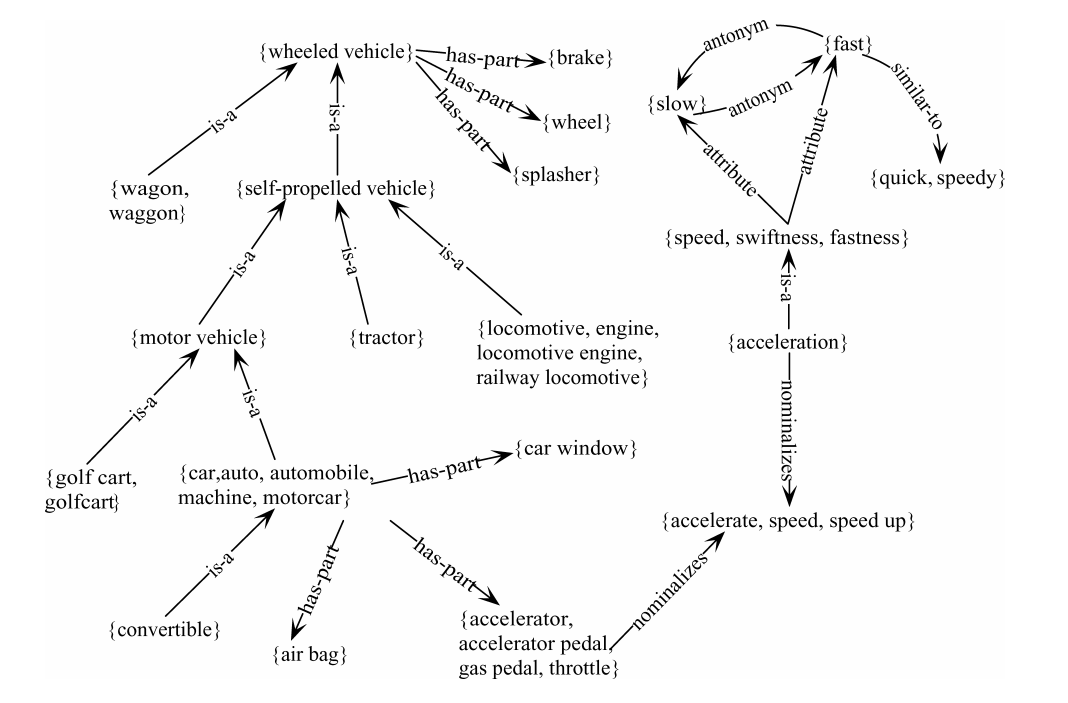
\includegraphics[scale = 0.6]{excerptFromWordNet.png}
\caption{Excerpt From WordNet}
\label{fig:excerptFromWordNet}
\end{center}
\end{figure}

\section{Problem Statement}
Formally, the task we are attempting has two objectives: 
\begin{enumerate}
\item Given a fine-grained sense inventory like WordNet, we wish to produce a clustering over WordNet synsets at any arbitrary granularity, which can serve as a coarse sense dictionary. 
\item Given a coarse sense inventory obtained by clustering fine-grained senses, assess its quality and show that it helps improve sense disambiguation on standard test sets.
\end{enumerate}

\section{Related Work}
\label{chapter:Background}
Systems using WordNet as the underlying ontology often suffer because of the fine-grained nature of the sense inventory. With more and more applications using WordNet, clustering word senses such that the application developer has the control over the granularity becomes very important.

\paragraph{}
One of the earliest attempt at coarsening of Machine Readable dictionaries was made by \citep{Dolan:1994}. 
They tried to discover similarities between senses of Longman's Dictionary of Contemporary English(LDOCE) using multiple heuristics based on a variety of information about a sense's meaning.

\paragraph{}
A wide variety of automatic methods have been proposed since then for coarsening fine-grained inventories. In this section, we discuss the approaches proposed in literature to coarsen sense inventories. The different ideas to cluster senses can be broadly categorized as follows: 
\begin{itemize}
\item Merging senses based on the sense ontology structure.
\item Clustering based on word sense similarity estimated from external corpora.
\item Exploiting Disagreements: between human annotators or between WSD systems.
\item Using translational equivalences of word senses.
\item Mapping to coarser sense inventories.
\item Clustering senses using supervision.
\end{itemize}

\subsection{Merging senses based on ontology structure}
\citep{peters1998automatic} suggest merging of two word senses based on structural cues derived from the ontology structure. They cluster senses which are connected by ontology based relations like  \textit{twins}\footnote{Two synsets having more than one word common.}, \textit{autohyponymy}\footnote{If one sense is a direct descendant of the other in the hypernym-hyponym ontology.}, 
\textit{sisters}\footnote{Word senses that share the same hypernym}, 
\textit{cousins}\footnote{Node pairs whose hyponyms exhibit a specific relation to each other: identified and listed by lexicographers in WordNet 1.5.} etc.
\citep{Mihalcea01ez.wordnet:principles} extended this idea and proposed six semantic principles to merge synsets and probabilistic principles to drop infrequent synsets.
Some interesting principles include merging synsets sharing a \textit{pertainym}, \textit{antonym} or sharing the same \textit{verb group}\footnote{Verb Groups are manually determined by lexicographers.}.
This was the first attempt to group synsets instead of word senses.

\paragraph{}
A number of synset similarity measures based on the WordNet structure have also been proposed in literature like 
Path Based Similarity Measures by \citep{WuPalmer:1994}, \citep{LCH:1998}, Information Content Based Measures by \citep{Resnik:1995}, \citep{JCN:1997}, \citep{Lin:1998} and Gloss Based Heuristics by \citep{Lesk:1986},\citep{Banerjee:2002}. We discuss these similarity measures in detail in Section \ref{section:similarityMeasures}.
Though these measures have not been used directly for WordNet sense clustering, they have motivated researchers in the NLP community to make full use of the WordNet structure to capture similarity between senses.

\subsection{Clustering based on Word Sense similarity estimated from External Corpora}
For estimating similarity between words, many corpus oriented attempts have been made like \citep{Pereira:93a}, \citep{Lin:1998}, \citep{kolb2008disco} and \citep{agirre2009study}. The problem with these approaches is that they are not able to handle the polysemous nature of words. Also, the dearth of sense annotated corpora prevents most of these methods to be used effectively in computing word sense similarities.

\paragraph{}
\citep{agirre2003clustering} associated a topical vector with each word sense, called \textit{Topic Signature}, which captures the relatedness between the target word sense and vocabulary. The cosine similarity between the vectors of two senses is used as the similarity between them. To calculate these vectors, they collect contexts for a polysemous words from manually sense-tagged corpora and by using instances of a polysemous word's monosemous relatives\footnote{Single-sense synsets related by hyponym, hypernym or any other relation of WordNet.} from large untagged corpora and the web. The idea behind the approach is that because of lack of sense annotated data, semantically close senses may not have a lot of direct shared contexts, but they are expected to have similar distributional neighbours.

\paragraph{}
On similar lines is the approach by \citep{mccarthy2006relating}. They calculate sense similarities using a combination of the JCN WordNet based similarity measure \citep{JCN:1997} and word-to-word distributional similarity. They introduce a more relaxed notion of sense relatedness which allows the user to control the granularity for the application in hand.

\subsection{Exploiting Disagreements: between WSD Systems or between Human Annotators}
The central idea involved here is that whenever good WSD systems or human annotators get confused while disambiguating, the senses they mark as answers are semantically related to the correct answer.
\begin{example} 
\label{example:fish}
Consider the following noun senses of the word \textit{fish}, taken from WordNet 3.1:
\begin{itemize}
\item fish (any of various mostly cold-blooded aquatic vertebrates usually having scales and breathing through gills) ``the shark is a large fish"

\item fish (the flesh of fish used as food) ``in Japan most fish is eaten raw"

\item Pisces, Fish ((astrology) a person who is born while the sun is in Pisces)

\item Pisces, Pisces the Fishes, Fish (the twelfth sign of the zodiac; the sun is in this sign from about February 19 to March 20)
\end{itemize}
\end{example}

It is unlikely that a human annotator mistags the astrology sense of the word \textit{fish} with its food sense. Similar results are expected from a good WSD system as well.

\paragraph{}
\citep{chklovski2003exploiting} derives confusion matrices exploiting the disagreements between human annotators and uses the same to generate coarse sense clusters. On the other hand, \citep{agirre2003clustering} uses the publicly available outputs of Senseval-2 \citep{Edmonds:2001} participants to construct the confusion matrices between word senses and then cluster them using hierarchial agglomerative clustering. Dearth of available manually sense-tagged data and not-so-high performance of the WSD systems limits the applicability of the above mentioned ideas.

\subsection{Using translational equivalences of word senses}
\citep{chugur2002polysemy} constructed similarity matrices for Senseval-2 \citep{Edmonds:2001} words based on translations of these words in four languages. The principle involved can be summed as: \textit{two word senses which are translated with the same word sense in other language are expected to be semantically similar}. Using multiple languages enables us to cover all the sense divisions offered by different languages. \citep{agirre2003clustering} uses the similarity matrices provided by \citep{chugur2002polysemy} and report resulting hierarchial clusters.

With the advent of WordNets being developed in multiple languages\footnote{GlobalWordNet lists the WordNets available in the public domains: \url{http://www.globalwordnet.org/gwa/wordnet_table.html}.} as well as multilingual ontologies like BabelNet \citep{NavigliPonzetto:12aij}, this seems a promising area which can help in coarsening of senses.


\subsection{Mapping to coarser sense inventories}
Mapping WordNet to other inventories either manually or automatically to generate coarse senses has also been tried by many researchers in the NLP community. When the different WordNet senses map to the same sense in the other ontology via manual mapping or automatic mapping, it is expected that the senses must have been semantically close. The underlying assumption being that the automatic mapping is able to capture the semantic similarity between the concepts in both the ontologies with high efficacy.

The attempts made in this direction include mapping WordNet to Hector Lexicon \citep{palmer2007making}, PropBank \citep{palmer2004different} and Levin Classes \citep{levin1993english} \citep{palmer2007making}. Most of these mappings are not complete in both directions, which hampers their utility.

The automatic approach presented by \citep{Navigli06meaningfulclustering} for mapping between sense inventories, WordNet to Oxford English Dictionary to be precise, is an elegant approach exploiting similarities in glosses and semantic relationships in the sense inventories. The approach can be extended to discover more semantic relationships in WordNet by using the ontology structure of the ontology mapped to WordNet.

\subsection{Clustering senses using supervision}
One of the earliest attempt to cluster senses using supervision was proposed by \citep{snow07mergesense}. They train a Support Vector Machine \citep{vapnikSVM:95} using features derived from WordNet and other lexical resources, whose predictions serve as a distance measure between synsets. For synset pairs with no common words, they assume a zero sense similarity score. They cluster synsets using average link agglomerative clustering and the synset similarity model learnt. While merging synsets to construct a coarse taxonomy, the merged synset inherits its hypernymy from its most frequent constituent sense. All other relationships are added to the new merged sense as long as the acyclic nature of the relations is conserved.

\section{Discussion}
In this section, we discuss some ideas which shaped the direction of our approach to the problem of WordNet sense clustering.

\subsection{Dropping Infrequent WordNet Synsets}
To reduce polysemy in WordNet, \citep{Mihalcea01ez.wordnet:principles} proposed to drop infrequent synsets, along with merging similar senses. They scored the synsets using frequency information of senses in SemCor \citep{SemCor} and dropped the low scoring synsets. 

We study the usefulness of this idea on the SemEval 2007 WSD test datasets \citep{navigli-litkowski:SemEval-2007}, in which we have three generic Wall Street Journal texts and two domain-specific documents (relating to computer programming and Italian painting respectively). Our scoring function is similar to the one proposed by \citep{Mihalcea01ez.wordnet:principles} and is given by:

\begin{equation}
Score(Synset) = \sum_{i \in Synset} Score(WordSense_i) 
\end{equation}

\begin{equation}
Score(WordSense) = \frac{Frequency(WordSense)+\alpha}{Frequency(LemmaWord) + \alpha*NumberOfSenses(LemmaWord)} 
\end{equation}

Here $\alpha$ is the Laplacian correction parameter(for our study we take $\alpha=1$).
The scoring function does not make reference to the component word senses directly and thus we do not have to deal with the data sparseness issue that arises from the limited size of the corpus.

We drop the synsets whose score is less than a threshold and study the number of instances for which the correct answer was removed, thus accounting for error. Since the task was on coarse grained WSD evaluation, we have multiple senses as the correct answer. In this case, we measure the fraction of senses removed from the set of correct senses for each of the instances. We report the error score calculated, weighted by the number of instances in the documents.

% \begin{center}
% \begin{longtable}{| c | c | c |}  
% \hline
% \textbf{Corpora Type} & \textbf{Threshold} & \textbf{Weighted Error Score} \\ \hline
% WSJ & 0.03 & 7.72 \\ \hline
% Domain & 0.03 & 10.48 \\ \hline
% WSJ & 0.06 & 13.91 \\ \hline
% Domain & 0.06 & 14.19 \\ \hline
% WSJ & 0.1 & 18.77 \\ \hline
% Domain & 0.1 & 19.13 \\ \hline
% \caption{Synsets Dropping Study}
% \label{tab:synsetsDroppingStudy}
% \end{longtable}
% \end{center}

\begin{center}
\begin{longtable}{cc|c|c|c|c}
\cline{3-5}
& & \multicolumn{3}{ c| }{Threshold} \\ \cline{3-5}
& & 0.03 & 0.06 & 0.1 \\ \cline{1-5}
\multicolumn{1}{|c }{\multirow{2}{*}{Corpora} } & \multicolumn{1}{ |c| }{WSJ} & 7.72 & 13.91 & 18.77 \\ \cline{2-5}
\multicolumn{1}{|c }{} & \multicolumn{1}{ |c| }{Domain} & 10.48 & 14.19 & 19.13 & \\ \cline{1-5}
\caption{Dropping Infrequent Synsets - A Comparision} 
\label{tab:synsetsDroppingStudy}
\end{longtable}
\end{center}


We observe that for lower thresholds, the error rate is higher for domain specific datasets whereas as we increase the threshold, thus removing more and more synsets, the error rates of both the datasets become comparable. The results match our expectation as we expect that some of the words in domain specific datasets would have low frequencies and thus low scores. To summarise, while working with text from the general domain, removing some infrequent synsets might improve the disambiguation but in case of domain specific datasets, it should not be done.

\subsection{Clustering Synsets Vs Clustering Senses}
For generating a coarse sense inventory, many researchers have focused on clustering WordNet senses into groups i.e. generate coarse senses for each word by merging its senses \citep{agirre2003clustering} \citep{chklovski2003exploiting} \citep{Navigli06meaningfulclustering}. In this approach, we would like to highlight two problems. One problem is that it requires a stopping criterion for each word such as the number of final classes. In literature, researchers have used the numbers determined by the available gold standard datasets for the purposes of evaluation \citep{agirre2003clustering}. As the right number of classes for each word cannot usually be predetermined even if the application is known, such coarsening systems cannot be used to derive coarse senses for all the words. The other problem is the inconsistent sense clusters obtained because of independent generation of coarse senses for each word. Even manually done sense clusterings can have this error: consider the sense groupings of the verbs \
textit{need} and \textit{require} from Senseval-2 judgements in figure \ref{fig:transitiveError} \citep{snow07mergesense}.

\begin{figure}[h]
\begin{center}
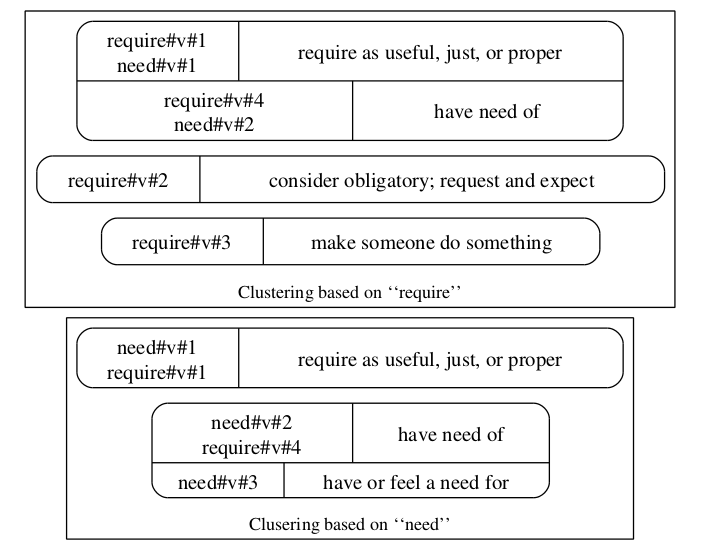
\includegraphics[scale = 0.6]{transitiveError.png}
\caption{Inconsistency in sense groupings for the verbs \textit{need} and \textit{require} from Senseval-2 judgements}
\label{fig:transitiveError}
\end{center}
\end{figure}

The two WordNet 2.1 senses \textit{need\#v\#1} and \textit{need\#v\#2} clustered in word specific labelling for \textit{require}, are not clustered in word specific labelling for \textit{need}. These transitive closure errors suggest that for deriving consistent coarse senses, we should cluster synsets and not senses.

\section{Evolution of Evaluation Frameworks}
We would like to highlight here the different frameworks used in literature for evaluating the sense clustering problem. Early systems studied the quality of clusters of word senses by studying polysemy degree of the text \citep{Mihalcea01ez.wordnet:principles} or by measuring the entropy and purity of the clusters obtained \citep{agirre2003clustering}.

Another idea is to compare the clustering obtained against a manually sense clustered dataset as done by \citep{chklovski2003exploiting}. This can be done by treating clustering as a pairwise classification task and reporting the F-Score for the classification task. The problem with this approach of evaluation is that the number of intra-cluster pairs is often small compared to inter-cluster pairs in clustering tasks. This imbalance could lead to understating pairwise similarity and can be avoided by using FScore for both the classes as performance evaluators.

The recent line of thought in evaluation is to go for a task based evaluation. \citep{mccarthy2006relating} studied the performance of first sense heuristics in the Senseval-2 English LS Task \citep{Senseval2LexicalSampleTask}. \citep{Navigli06meaningfulclustering} and \citep{snow07mergesense} assess the effect of automatic sense clustering on the three best-ranking WSD systems of the English AW task at Senseval-3 \citep{Senseval3AllWordsTask}. Since the main motive for coarsening WordNet inventory is to make WSD a plausible task, studying the performance of sense disambiguation systems on automatically generated coarsened senses seems a well founded approach.

\section{Broad Overview of our Approach}
We propose a framework which derives a coarse sense inventory by learning a synset similarity metric. We focus on the coarsening of noun synsets of WordNet and show that the coarse-grained sense inventory obtained notably improves the disambiguation of nouns.

Our approach closely resembles \citep{snow07mergesense} as far as supervised learning of the synset similarity is concerned. But to learn synset similarity of synset pairs which don't share a word, instead of giving them zero similarity, we learn it using a variant of the SimRank framework \citep{Jeh02simrank}. 

Also, \citep{snow07mergesense} proposes to modify the WordNet ontology structure to produce a coarse version of WordNet; however we argue on the lines of \citep{mccarthy2006relating} that a softer notion of relationships between senses should be used compared to fixed groupings so that the variable granularity needs of different applications can be met.

\begin{comment}
\subsection{Understanding sense clustering}
When we merge two synsets, should we modify the underlying structure of taxonomy as well?
What should be the repercussion of the mergings on the taxonomy?

An important point to note here is that if we merge two synsets and introduce the merged synsets instead of the original synsets in the WordNet taxonomy, either we'll be adding some spurious relations and/or we'll be losing some relationship information.

\end{comment}

\section{Organization of Thesis}
In this chapter, we introduced the problem, reviewed the algorithms proposed for the task of sense clustering and the evaluation frameworks for the same. 
The rest of this thesis is organized as follows. 
Chapter \ref{chapter:SupervisedSynsetSimilarity} discusses a supervised attempt to capture WordNet synset similarity using various features derived from WordNet and external corpora. 
Chapter \ref{chapter:Semi-SupervisedSynsetSimilarity}, presents a semi-supervised approach to estimate WordNet synset similarity using a variant of SimRank \citep{Jeh02simrank} and describes our approach to produce a coarse sense inventory. 
The conclusions and future work are part of chapter \ref{chapter:conclusion}.

	\chapter{Related Work}
\label{chapter:relatedwork}
The task of text classification, i.e. classification of documents into a fixed number of predefined categories has been long studied in-depth for many years now. This multi-class classification problem has further evolved into a multi-label text classification task where each document can belong to multiple, exactly one or no category at all. 

Supervised machine learning techniques that learn classifiers to perform this category assignment task can be broken down into two main components, namely, text representation and learning algorithm. 
Text representation involves converting the documents, that are usually strings of characters, into numerical vectors that are suitable inputs to the learning algorithm while the learning algorithm uses pairs of labeled input text representations and the categories it is belongs in, to learn a model so as to classify new documents into categories.

\section{Text Representation}
\label{sec:textrepr}
Any text-based classification system requires the documents to be represented in an appropriate manner dictacted by the task being performed \citep{lewis1992text}. Moreover, \citep{quinlan1983learning} showed that the accuracy of the classification task depends as much on the document representation as on the learning algorithm being employed. Different from the data mining task, which deals with structureed documents, text classification deals with unstructured documents that need to be appropriately transformed into numerical vectors, i.e. the need for text representation. In this section we introduce the most effective and widely-used techniques to represent documents for text classification.

\subsection{Bag of Words}
It is found in information retrieval research that word stems work well as representations units for documents and that their ordering in a document is of minor importance for many tasks. This is attributed by the fact that the most widely-used used model to represent documents for the classification task is the \emph{Vector Space Model (VSM)} \citep{salton1973specification}. 

In the Vector Space Model, a document $d$ is represented as a vector in the term/word space, $d$ $=$ $(w_{1}, w_{2}, \ldots, w_{|V|})$ where $|V|$ is the size of the vocabulary. Each of the $w_{i} \in \left[0,1\right]$, represents the weightage of the term $i$ in the document $d$. This is called the \emph{bag-of-words} model as it ignores word ordering and each document is reduced to a bag of words that it contains or not. 

An important requirement of such a representation is that, the terms that help in defining the semantic content of the document and play an important role in classification be given higher weightage than the others. Over the years, there has been much research in the information retrieval field on term weighting schemes. The most important term-weighting techniques are described below : 
\begin{enumerate}
\item{\textbf{One Hot Representation} : }This is the most trivial representation, where each document is represented by a vector that is size of the vocabulary. Each element in the vector is either a $0$ or a $1$ to denote the absence or presence of a specific term in the document.

\item{\textbf{Term Frequency (tf))} : }The term frequency representation weighs the terms present in the document relative to their occurence frequency in the document. Hence a document $d$ is represented as, $d$ $=$ $(w_{1}, w_{2}, \ldots, w_{|V|})$, where, $w_{k}$ is the number of times the term $k$ appears in the document $d$. 
% \begin{equation}
% w_{i} = \frac{N_{i,d}}{N_{d}}
% \end{equation}
% where, $N_{i,d}$ is the number of times, term $i$ occurs in document $d$ and $N_{d}$ is the total number of terms in the document. The document can also be represented only by the counts of terms, but normalization is done to reduce the effect of document length.
\item{\textbf{Inverse Document Frequency (idf)} : }Though using \emph{tf} as a term weighting scheme is a good starting point, it faces a challenge when high frequency terms are not concentrated in a few particular documents but are prevalent in the whole collection. Those terms then stop being characteristic of the semantic content of a few documents and need not be given high weightage. To overcome this problem, \cite{salton1988term} suggested a new term weighting called the inverse document frequency (idf). The \emph{idf} weight of a term varies inversely with the number of documents $n$ it belongs to in a collection of total $N$ documents. A typical \emph{idf} vector can be computed as 
\begin{equation}
w_{k} = \log \frac{N}{n}
\end{equation}
\item{\textbf{Term Frequency Inverse Document Frequency (tf-idf)} : }Given the above two term weighing schemes, it is clear that an important term in a document should have high \emph{tf} but a low overall collection frequency (\emph{idf}). This suggests that a reasonable measure for term importance may be then obtained by the \emph{tf} and the \emph{idf} (\emph{tf}$\times$\emph{idf}). As we will see in the results section, the \emph{tf-idf} weighed bag-of-words document representation gives one of the best accuracies in the multi-label text classification task.
\end{enumerate}
% \subsubsection{One Hot Representation}
% This is the most trivial representation, where each document is represented by a vector that is size of the vocabulary. Each element in the vector is either a $0$ or a $1$ to denote the absence or presence of a specific term in the document.

% \subsubsection{Term Frequency (tf))}
% The term frequency representation weighs the terms present in the document relative to their occurence frequency in the document. Hence a document $d$ is represented as, $d$ $=$ $(w_{1}, w_{2}, \ldots, w_{|V|})$, where, $w_{k}$ is the number of times the term $k$ appears in the document $d$. 
% % \begin{equation}
% % w_{i} = \frac{N_{i,d}}{N_{d}}
% % \end{equation}
% % where, $N_{i,d}$ is the number of times, term $i$ occurs in document $d$ and $N_{d}$ is the total number of terms in the document. The document can also be represented only by the counts of terms, but normalization is done to reduce the effect of document length.
% \subsubsection{Inverse Document Frequency (idf)}
% Though using \emph{tf} as a term weighting scheme is a good starting point, it faces a challenge when high frequency terms are not concentrated in a few particular documents but are prevalent in the whole collection. Those terms then stop being characteristic of the semantic content of a few documents and need not be given high weightage. To overcome this problem, \cite{salton1988term} suggested a new term weighting called the inverse document frequency (idf). The \emph{idf} weight of a term varies inversely with the number of documents $n$ it belongs to in a collection of total $N$ documents. A typical \emph{idf} vector can be computed as 
% \begin{equation}
% w_{k} = \log \frac{N}{n}
% \end{equation}
% \subsubsection{Term Frequency Inverse Document Frequency (tf-idf)}
% Given the above two term weighing schemes, it is clear that an important term in a document should have high \emph{tf} but a low overall collection frequency (\emph{idf}). This suggests that a reasonable measure for term importance may be then obtained by the \emph{tf} and the \emph{idf} (\emph{tf}$\times$\emph{idf}). As we will see in the results section, the \emph{tf-idf} weighed bag-of-words document representation gives one of the best accuracies in the multi-label text classification task.

% A common feature in the bag-of-words document representation is the \emph{normalization factor}\citep{salton1988term} introduced to reduce the effect of varying document lengths and give equal weightage to documents of all lengths when learning the classifier for text categorization. \todo{Do we put how normalization is done?}
% Another feature added to the bag-of-words representation is the removal of stop-words (short function words that do not add to the semantic content of the document) and words that occur infrequently to make the document vector more meaningful.

\subsection{Dimensionality Reduction / Feature Selection}
The bag-of-words representation scheme has several drawbacks but the most important drawback it suffers from is that document vectors are very sparse and high dimensional. Typical vocabulary sizes of a moderate-sized document collection ranges from tens to hundereds of thousands of terms which is prohibitively high for many learning algorithms. 
To overcome this issue of high-dimensional bag-of-words document representations, automatic feature selection is performed that removes uninformative terms according to corpus statistics and constructs new orthogonal features by combining several lower level features (terms/words). Several techniques used in practice are discussed below, 
\begin{enumerate}
\item{\textbf{Information Gain} : }Information Gain is widely used as a term-goodness criterion in the field of machine learning, mainly in decision trees \citep{quinlan1986induction} and also in text classification \citep{lewis1994comparison}, \citep{moulinier1996text}. It is a feature space pruning technique that measures the number of bits of information obtained(entropy) for category prediction by knowing the presence or absence of a term in a document. For terms where the information gain was below some predefined threshold are not considered in the document vector representation.  The information gain of a term $t$ is defined as
\begin{equation}
G(t) = -\sum_{i=1}^{|C|} P(c_{i})\log P(c_{i}) + P(t)\sum_{i=1}^{|C|} P(c_{i}|t)\log P(c_{i}|t) + P(~t)\sum_{i=1}^{|C|} P(c_{i}|~t)\log P(c_{i}|~t)
\end{equation}

\item{\textbf{Mutual Information} : }Similar to the Information Gain scheme, Mutual Information estimates the information shared between a term and a category and prunes terms that are below a specific threshold. The mutual information between a term $t$ and a category $c$ is estimated in the following fashion, 
\begin{equation}
I(t,c) = \log \frac{P(t \wedge c)}{P(t) \times P(c)}
\end{equation}
To measure the goodness of a term in global feature selection, the category specific scores of a term are combined using, 
\begin{equation}
I_{avg}(t) = \sum_{i=1}^{|C|} P(c_{i})I(t,c_{i})
\end{equation}

\item{\textbf{$\chi^{2}$ Statistic} : }The $\chi^{2}$ statistic measures the lack of independence a term $t$ and a category $c$ and can be compared to the $\chi^{2}$ distribution with one degree of freedom. The term-goodness factor is calculated for each term-category pair and is averaged as above. The major difference between Mutual Information and $\chi^{2}$ statistic is that the later is a normalized value and the goodness factors across terms are comparable for the same category.

\item{\textbf{Latent Semantic Indexing (LSI)} : } LSI first introduced by \cite{deerwester1990indexing}, is a popular linear algebraic dimensionality reduction technique that uses the term co-occurence statistics to capture the latent semantic structure of the documents and represent them using low-dimensional vectors. It is an efficient technique to deal with synonymy and polysemy. LSI aims to find the best subspace approximation to the original document bag-of-word vector space using Singular Value Decomposition. Given a term-document matrix $X = \left[ x_{1}, x_{2}, \ldots, x_{|D|} \right] \in \mathbb{R}^{|V|}$, its k-rank approximation as found using SVD, can be expressed as, 
\begin{equation}
X = T S D^{T}
\end{equation}
where, $T \in \mathbb{R}^{|V| \times k}$ and $D \in \mathbb{R}^{|D| \times k}$ are orthonormal matrices called the left and right singular vectors respectively. The matrix $S \in \mathbb{R}^{k \times k}$ is a diagonal matrix of singular values arranged in descending order. The $k$-dimensional rows of the matrix $D$ contain the dimensionality reduced representations of the $|D|$ documents in the collection. The representations obtained using LSI alleviate the issue of data sparsity and high-dimensionality in bag-of-words representations and also helps unfold the latent semantic structure of the documents.
\end{enumerate}

\section{Learning Algorithms}
\label{sec:lalgos}
Multi-label text classification has seen growing number of statistical learning methods being applied to it. Over the years, various larning algorithms like, Regression models (\citep{cooper1994full}, \citep{fuhr1991air}), Conditional Random Field (\citep{ghamrawi2005collective}), Nearest Neighbour techniques (\citep{yang1994expert}, \citep{zhang2005k}, \citep{zhang2007ml}), Bayesian classifier and topic modelling (\citep{lewis1994comparison}, \citep{mccallum1999multi}, \citep{nigam2000text}, \citep{rubin2012statistical}, \citep{nigam1999using}, \citep{ueda2002parametric}), SVM (\citep{joachims1998text}, \citep{elisseeff2001kernel}), Neural Networks (\citep{wiener1995neural}, \citep{ng1997feature}), Decision Trees (\citep{tong1994machine}), Online learning algorithms (\citep{lewis1996training}, \citep{crammer2002new}), Non-negative Matrix Factorization (\citep{liu2006semi}) etc. have been used or developed for Multi-label document categorization.

Earlier learning algorithms reduced the problem of multi-label classification into multiple binary classification problems and independently learned binary classifiers for each category. While these algorithms performed well, their drawback of considering correlation among categories led to the development of algorithms that learn a single classifier and jointly classify each document. 

Multi-label classification problems can be also be classified into classification-based and ranking-based approaches, where the former assigns each test instance a $|L|$-sized label vector of ones and zeros indicating the presence and absence of labels. In the case of a ranking-based approach, the ranking system outputs the list of labels arranged in the increasing order of a ranking score which is then thresholded at an optimum and the top labels are considered appropriate label assigments for test instances.

Below we describe some of the famous learning algorithms for multi-label text classification, 

\subsection{With Multiple Binary Classifiers}
\label{sec:rw_multiple_classifiers}
The most common approach of multi-label text classification treats each label independently and learns multiple binary classifiers, one for each category and then assigns to a test document all the categories for which the corresponding classfier says \emph{`yes'}. Below we describe some of the algorithms, in the context of multi-label text classification, that learn multiple independent binary classifiers.
\begin{enumerate}
\item{\textbf{Logistic Regression (LR)} : }Introduced by \citep{hosmer1989applied}, LR is a probabilistic binary classification regression model, that, for binary text classification learns a category weight vector and estimates the probability of a document belonging to the category using dot-product and the logistic link function. LR can be extended for multi-label document classification by learning multiple category vectors, specifically, one for each category. At test time, one would need to query all category vectors for each document to make the category assignments. In our work, we use logistic regression for multi-label text classification, the details for which are given in Sec~\ref{sec:lrtc}.

\item{\textbf{Support Vector Machines (SVM)} : } Support Vector Machines (\citep{cortes1995support}, \citep{vapnik2000nature}) based on the \emph{Structural Risk Minimization} principle, are universal learners. In their basic form, SVMs learn linear threshold functions to find linear hyperplanes in the input data space to separate data of the two differnt classes. In the case, where data is not linearly separable, SVMs can be plugged-in with appropriate kernel functions to learn polyniomial classifiers, radial basic fucntions etc. For multi-label text classification, training data is treated separately for each category and maximum margin separating hyperplanes are found for each category independently \citep{joachims1998text}.

\cite{elisseeff2001kernel} study a ranking based variant of SVM, where the positive/negative distance from the separating hyperplane of a specific category is the score assigned to the particular instance for that category. Their formulation then aims to maximize the margin between the score of a category that belongs to the document and a category that does not belong to do the document. This is also called the Rank-SVM.

\item{\textbf{Neural Networks (NNet)} : }Classification-baed, Neural Network approaches to multi-label text classification were mainly studied by \cite{wiener1995neural}, developed at Xerox PARC and called NNet.PARC and \cite{ng1997feature}, called CLASSI. Both neural networks are examples of multiple-classifier based approaches where a separate neural network was trained for each category to make binary classifications. While CLASSI used a linear perceptron approach to classify text into categories, NNet.PARC built a three-layered nonlinear neural network that extends logistic regression by modelling higher order term interactions and hence finding non-linear decision boundaries. 

\item{\textbf{Naive Bayes (NB)} : }Naive-bayes as studied in \cite{lewis1992representation} and \cite{lewis1994comparison}, is one of the most effective and simple statistical model for text classification. For multi-label classification, classifiers are learnt so as to estimate $P(C_{j}=1|D)$, i.e., the probability that the document, $D$ belongs to the category $C_{j}$, for each category. This probability is estimated by estimating the probability $P(W_{i}=1|C_{j}=1)$, i.e. probability that a particular word appears in the document when it belongs to a particular category. Though this approach makes the assumption of word independence, experiments show that this fast-learning algorithm can yield excellent results. 
\end{enumerate}
Although, approaches to multi-label classification discussed above give competitive accuracies in the task, they suffer from inefficiencies due to the following reasons,
\begin{itemize}

\item make assumptions of category independence and learn 1-vs-All binary classifiers. It is realized that such assumption would not hold true in most real-life situations. Fine-grained categorization of texts usually involve strongly correlated category classes and information about the presence of one gives information about the presence/absence of many others. For eg. in the sentence, 
\begin{quote} 
\centering 
\emph{Chicago Board of trade grain traders and analysts voiced a lot of interest in how farmers planned to handle their upcoming spring plantings prompting sales of new crop months of corn and oats and purchases in new crop soybeans in the futures markets}
\end{quote}
information from words about the presence of categories like \emph{oats}, \emph{corn} etc. can also aid the prediction of the \emph{agriculture} category which can be boosted using joint classification.
\end{itemize}
Apart from inefficiencies induced by ignoring category correlations, learning independent classifiers poses other drawbacks, such as, in case of millions of labels, learning millions of high-dimensional classifiers is a computationally expensive. Secondly, the cost of prediction for each test instance would be high as all the classifiers need to be evaluated to make a single prediction.


\subsection{With Single Joint Classifier}
To overcome the difficulties and drawback of learning multiple binary classifiers, researchers have since developed learning algorithms that jointly classify each document into categories it belongs to. Outputs of such algorithms are $|L|$-dimensional label vectors $\boldsymbol{y} \in \{0, 1\}^{L}$, with $\boldsymbol{y}_{l} = 1$ if label $l$ is relevant for the particular document. Below we describe algorithms for multi-label text classification that learn a single classifier for assigning all relevant labels to a document jointly.
\begin{enumerate}
\item{\textbf{k-Nearest Neighbor (kNN)} : }k-nearest neighbor classification is one of the most effective lazy learning approaches to classification. Given an arbitrary text document input, the algorithm first ranks the nearest neighbors among the training documents using some similarity measure. It then uses the category information of the top-k ranked nearest neighbors to predict the categories of the input test document. One simple approach is to take a weighted average of the label vector of the k-nearest neighbors, weights being the similarity score while estimating document distances. This yields a category ranking for the test input which can be thresholded to yield binary classifications.

Other approach as devised by \cite{zhang2007ml} is based on the k-NN and the maximum a posteriori(MAP) principle. Their approach is, given a test instance, to first identify its k-nearest neighbors and then based on the statistical information gained from the label sets of the neighboring instances, use the MAP principle to determine the label set of the given input. The prior probability of label occurences and the posterior probability, $P(C_{l}=n | l=1)$ i.e. given a document belongs to label $l$, exactly $n$ of its $k$ neighbors also belong to the label $l$ is determined from the training instances to utilize the MAP principle.

\item{\textbf{Linear Least Squares Fit (LLSF)} : }LLSF\citep{yang1992linear} learns a multivariate regression model automatically from a training set of documents and their categories. Documents are input as vectors in the desired representation and the corresponding output is a $|L|$-dimensional binary label vector. By solving a linear least squares fit on the training pairs of vectors a matrix of word-category regression coefficients is learnt, which defines the mapping from an arbitrary document to a weighted category label vector. This weighted vector can be sorted to yield a ranked list of categories for the input document.

\item{\textbf{Probabilistic Models} : }Generative probabilistic models described in \cite{mccallum1999multi}, \cite{nigam1999using}, \cite{ueda2002parametric} etc. argue that the words in a document belonging to a multi-category class can be regarded as a mixture of characteristic words related to each of the categories. Therefore, they represent the multi-label nature of the document by specifying each document with a set of mixture weights, one for each class and also indicate that each document is generated by a mixture of word distributions, one distribution for each label. Once the word distributions are learnt using the training data, classification is performed using the Bayes Rule which selects the labels that are most likely to generate the given test document. Hence, along with giving the information on the labels responsible for generating the document, such models also fill the missing information of which labels were responsible for generating each word.

\cite{mccallum1999multi} and \cite{ueda2002parametric} define a multinomial distribution $\boldsymbol{\theta}_{l} = \{\theta_{l1}, \theta_{l2}, \ldots, \theta_{l|V|}\}$ over the vocabulary for each label, and the word distribution for a document for a given label vector $\boldsymbol{y}$, is computed by taking a weighted average of the word distributions of the labels that are present in the document. Therefore, if $\boldsymbol{\phi}(\boldsymbol{y}) = \{\phi_{1}(\boldsymbol{y}), \phi_{2}(\boldsymbol{y}), \ldots, \phi_{2}(\boldsymbol{y})\}$ is the required word distribution, it can be representated by, 
\begin{equation}
\boldsymbol{\phi}(\boldsymbol{y}) = \sum_{l=1}^{|L|} h_{l}(\boldsymbol{y})\boldsymbol{\theta}_{l}
\end{equation}
where $h_{l}(\boldsymbol{y})$'s are the mixing proportion that add upto $1$. The word distributions for each label are found by maximizing the posterior in \citep{ueda2002parametric} and by employing the Expectation-Maximization algorithm in \citep{mccallum1999multi}.

\end{enumerate}

	%\chapter{Supervised Synset Similarity}
\label{chapter:SupervisedSynsetSimilarity}
In this chapter, we describe a supervised attempt at learning synset similarity in which we train a Support Vector Machine using a semantically rich collection of features obtained from the WordNet ontology and other publicly available lexical resources connected to WordNet.

\section{Motivation}

%Learning synset similarity using supervision has twofold motivation.

Most of the synset similarity measures, like JCN \citep{JCN:1997}, LCH \citep{LCH:1998} etc., proposed in literature are generally unsupervised, relying mostly on WordNet structure and raw text corpora. Our aim in this chapter is to provide a supervised alternative to the above mentioned approaches, which utilizes the WordNet structure to its fullest and makes use of additional resources like WordNet Domains \citep{Gonzalez:XWND}, SemCor \citep{SemCor}, SentiWordNet \citep{Baccianella10sentiwordnet3.0} etc as well. 

%Significant advancement of supervised learning algorithms over the last two decades

Supervised systems allow us to intelligently combine and weigh the different features and thus give us an insight into how humans relate word senses.

\section{Algorithm Outline}
\label{sec:supervisedAlgoOutline}
We formulate sense merging as a binary classification problem and tackle the same using supervision. We obtain pairs of synsets which human-annotators have labeled as ``merged'' or ``not merged'' and describe each pair as a feature vector. We learn a synset similarity measure by using a maximum margin classifier on this extracted dataset, where positive examples are the pairs which were merged and negative examples are the ones which were not merged by the annotators. The output value of the classifier for a synset pair is the learnt estimate of the similarity between synsets constituting the pair.

\section{Gold standard sense clustering data}
\label{section:goldStandardDatasets}
In this section, we will discuss the gold standard sense clustering datasets, the preparation of the pairwise classification datasets from them and the quality of these datasets.

Since our methodology depends upon the availability of labelled judgements of synset relatedness, the datasets involved are of paramount importance. 
We use the following manually labelled WordNet sense groupings:
\begin{itemize}
\item Sense groupings over WordNet senses provided by the Senseval-2 English LS task organizers  \citep{Senseval2LexicalSampleTask}.
\item Mappings from the Omega ontology \citep{philpot2005omega} to the WordNet senses, provided by the OntoNotes project \citep{Hovy:2006}
\end{itemize}

\subsection{Senseval-2 Dataset}
Hand labelled sense clusters on selected nouns, verbs and adjectives was provided by the Senseval-2 English LS Task on WordNet 1.7 \citep{Senseval2LexicalSampleTask} \citep{Edmonds:2001}. 

\paragraph{Structure of dataset}: Let us consider the sense groupings of the noun \textit{air} given below. Annotator(s) have divided 8 senses of the word \textit{air} in 5 groups. The first group consists of 4 senses and the remaining groups consists of one sense each.

\begin{verbatim}
air%1:15:00:: 4 air%1:27:00::
air%1:19:00:: 4 air%1:27:00::
air%1:27:01:: 4 air%1:27:00::
air%1:04:00::
air%1:10:02::
air%1:07:00::
air%1:10:01::
\end{verbatim}

\paragraph{Binary Classification Data Generation}: From these clusters we generate a binary classification dataset where the task in hand is to label a pair to be merged or not. 
The process of extracting pairs is as follows: 
\begin{itemize}
\item Part of speech based separation of the word senses was done for convenience. Thus we obtained clusters of senses for each POS (noun, verb, adjective and adverb).
\item We map all these word senses to WordNet 3.0 synsets and get the clusters over synsets.\footnote{We use the mappings provided by the WordNet project and provided by Dr. Rada Mihalcea \url{http://www.cse.unt.edu/~ rada/downloads.html\#wordnet}}
\item Among all possible pairs from the obtained synsets, if both the offsets are present in the cluster, we label the pair as positive/merged, negative/not-merged otherwise.
\end{itemize}

\paragraph{Statistics}: 
The statistics related to the pairs obtained is tabulated in table \ref{tab:senseval2stats}. There was no pair for any of the POS which was in negative examples as well as positive examples.

\begin{center}
\begin{longtable}{| c | c | c | c |}  
\hline
POS & Positive example count & Negative example count & Fraction of positive examples \\ \hline
Noun & 119 & 552 & 0.22 \\ \hline
Verb & 477 & 4769 & 0.10 \\ \hline
\caption{Senseval-2 Pairwise Data Statistics}
\label{tab:senseval2stats}
\end{longtable}
\end{center}


\paragraph{Quality of Dataset}:
Unfortunately, no information about the dataset construction is known nor any inter-annotator agreement is reported in literature.

\subsection{OntoNotes Dataset}
\label{sec:OntoNotesDataset}
We use OntoNotes \citep{Hovy:2006} Release 3.0 \footnote{\url{http://www.ldc.upenn.edu/Catalog/docs/LDC2009T24/OntoNotes-Release-3.0.pdf}} for extracting WordNet sense clusters.\footnote{The OntoNotes groupings will be available through the LDC at \url{http://www.ldc.upenn.edu}} 

\paragraph{Structure of Dataset}: The dataset consists of senses for selected words in sense files. The senses in OntoNotes are mapped to WordNet senses, if a good mapping between senses exists.

\paragraph{Binary Classification Data Generation}: The steps involved in extraction are as follows:
\begin{enumerate}
\item Simplifying Dataset: We extracted the relevant portions of the sense inventories i.e. the mapping from OntoNotes senses to WordNet senses.
\item Version wise separation: 
  \begin{itemize}
  \item OntoNotes has mappings to 4 WordNet versions: 1.7, 2.0, 2.1 and 3.0. 
  \item We partitioned the inventory according to the versions. 
  \item We manually resolved the cases containing multiple versions of wordnet in a single sense file.
  \item We dropped monosemous words as there is no clustering possible in such cases.
  \end{itemize}
\item Mapping senses to WordNet 3.0: 
  \begin{itemize}
  \item We dropped WN1.7 as there were very few senses and the mapping from WN1.7 to WN3.0 was not easily available. \footnote{Mapping could have been obtained by using following mappings: WN1.7 to WN1.7.1 , WN1.7.1 to WN2.0, WN2.0 to WN2.1 and then WN2.1 to WN3.0.}
  \end{itemize}
\item Validating clusters on WN3.0: 
  \begin{itemize}
   \item We removed the sense files which did not contain all the senses of the word i.e. the clustering was not complete.
   \item We removed the sense files in which the clusters had a clash i.e. one sense belonged to multiple clusters.
   \item We removed the sense files in which there were invalid offset mappings.
  \end{itemize}
\item Removing Disagreements: We removed the instances from the dataset which were present in both positive and negative examples. This situation arises because the annotators were working with word senses and there were inconsistent sense clusters.
\end{enumerate}

\paragraph{Statistics}:
\begin{itemize}
\item \textbf{Number of Sense Files}: Effect of processing on number of sense files
\begin{center}
\begin{longtable}{| c | c | c |}  
\hline
    Stage & Noun & Verb \\ \hline
    Before Processing & 2033 & 2156 \\ \hline
    After processing & 1680 & 1951 \\ \hline
    \caption{Effect of processing on sense files}
\end{longtable}
\end{center}

\begin{comment}
% Not useful here
\item \textbf{Distribution of Sense Files}: Distribution of sense files across WN Versions
\begin{center}
\begin{longtable}{| c | c | c |}  
    \hline
    WN Version & Noun & Verb \\ \hline
    2.0 & 216 & 0 \\ \hline
    2.1 & 866 & 928 \\ \hline
    3.0 & 598 & 1023 \\ \hline
\end{longtable}
\end{center}
\end{comment}

\item \textbf{Average Polysemy Degree}: Average Polysemy Degree is defined as the average polysemy degree of the words weighted by their frequency in a large corpus. The equation \ref{eq:AveragePolysemyDegree} defines the same \footnote{Frequency of a word is the sum of the frequencies of all its sense occurrences, which we obtain from WN3.0.}. 
\begin{equation}
\label{eq:AveragePolysemyDegree}
AvgPolyDeg = \frac{\sum_i polysemyDegree(word_i) * freq(word_i)}{\sum_i freq(word_i)} 
\end{equation}

Average Polysemy degree of words in the cleaned dataset: 
\begin{center}
\begin{longtable}{| c | c | c |}  
    \hline
    Stage & Noun & Verb \\ \hline
    Fine & 5.28 & 9.55 \\ \hline
    Coarse & 4.10 & 3.97 \\ \hline
    \caption{Average Polysemy Degree of Cleaned OntoNotes dataset}
\end{longtable}
\end{center}

For comparison purposes, we would like to report the average polysemy degree in the dataset released for Semeval-2007 task \citep{navigli-litkowski:SemEval-2007} on coarse grained WSD. It is based on Wordnet 2.1 and was created automatically as described in \citep{Navigli06meaningfulclustering}. The dataset consists of only polysemous entries of which there are 11052 nouns and 4121 verbs.

\begin{center}
\begin{longtable}{| c | c | c |}  
    \hline
    Stage & Noun & Verb \\ \hline
    Fine & 3.76 & 5.84 \\ \hline
    Coarse & 2.18 & 2.54 \\ \hline
    \caption{Average Polysemy Degree of SemEval-2007 clustering}
\end{longtable}
\end{center}
%Average Noun Polysemy in Fine Senses 3.7587288018985547
%Average Noun Polysemy in Coarse Senses 2.175520889190637
%Average Verb Polysemy in Fine Senses 5.838670049134424
%Average Verb Polysemy in Coarse Senses 2.544635325109156
\end{itemize}

\paragraph{Binary Classification Dataset}
From the word sense clusters, we obtained the pairwise classification data for both nouns and verbs separately using the method described in \ref{sec:OntoNotesDataset}.
\begin{center}
\begin{longtable}{| c | c | c |}  
    \hline
    Statistics & Nouns & Verbs \\ \hline
    Number of Word Sense Files & 1680 & 1951 \\ \hline
    Distinct Offsets encountered & 4930 & 6296 \\ \hline
    %DOChoose2 & 12149985 & 19816660 \\ \hline
    %Positive Examples & 1253 & 7147 \\ \hline %before removing disagreements
    %Negative Examples & 12043 & 21142 \\ \hline
    Positive Examples & 1214 &  6881\\ \hline
    Negative Examples & 11974 & 20899 \\ \hline
    Percentage of Positive examples & 9.20 & 24.76 \\ \hline
    \caption{Statistics of Pairwise Classification Dataset obtained from OntoNotes}
  \label{tab:ontoNotesPairwiseData}
\end{longtable}
\end{center}

\paragraph{Quality of Dataset}:
The OntoNotes dataset creation involved a rigourous annotation process, in which around 50 examples for every target noun or verb were tagged with a preliminary set of senses. This process was continued until an ITA of atleast 90\% was reached, and in each iteration, the sense groupings were revised by the linguists and the examples were tagged again. Thus, using the coarse sense inventory of the final iteration, an ITA of at least 90\% is guaranteed on the sense-tagging of the sample sentences, which makes the quality of the final clustering of senses reasonably high. The process is summarised in figure \ref{fig:ontonotes}.

\begin{figure}[h]
\begin{center}
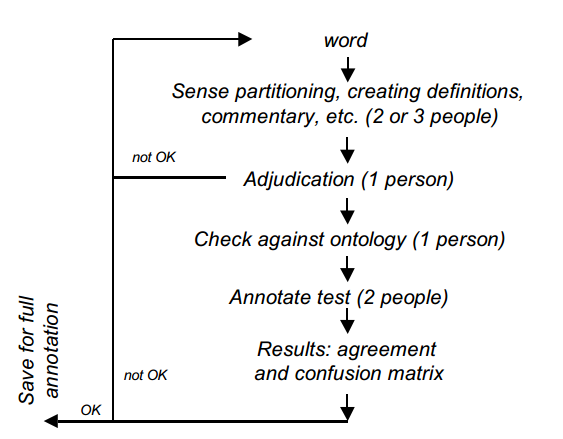
\includegraphics[scale = 0.6]{ontonotes.png}
\caption{OntoNotes Annotation Procedure \citep{Hovy:2006}}
\label{fig:ontonotes}
\end{center}
\end{figure}

\section{Feature Engineering}
\label{section:featureEngineering}
In this section, we describe the feature space construction. We derive features from the structure of WordNet and other available lexical resources. Our features can be broadly categorized into two parts: derived from WordNet and derived from other corpora.  WordNet based features are further subdivided into similarity measures and features. 
Many of the listed features are motivated by \citep{snow07mergesense} and \citep{Mihalcea01ez.wordnet:principles}.

\subsection{WordNet based Features}
\subsubsection{Similarity Measures} 
\label{section:similarityMeasures}
\begin{enumerate}
\item \textbf{Wu and Palmer's Conceptual Similarity}: WUP Similarity \citep{WuPalmer:1994} between concepts $a$ and $b$ in a hierarchy, given as
\begin{align}
sim_{WUP}(a,b) = \frac{2 \times depth(lso(a,b))}{len(a,lso(a,b)) + len(b,lso(a,b)) + 2 \times depth(lso(a,b))} \label{eq:WUP}
\end{align}

Here $depth(lso(a,b))$ is the global depth of the lowest super ordinate of $a$ and $b$ and $len(a,b)$ is the length of the path between the two nodes $a$ and $b$ in the hierarchy.

\item \textbf{Leacock and Chodorow's Normalized Path Length}: LCH Similarity \citep{LCH:1998} between concepts $a$ and $b$ in a hierarchy is given by:
\begin{align}
 sim_{LCH}(a,b) = -\log\left(\frac{len(a,b)}{2 \times \underset{c \in WordNet}{\mbox{max}} depth(c)}\right) \label{eq:LCH}
\end{align}

\item \textbf{Resnik's Information Theory Based Approach}: Information Content for a concept $C$ in the taxonomy is defined as $-\log_2p(c)$, where $p(c)$ is the probability of encountering an instance of concept $c$. Resnik's similarity, introduced in \citep{Resnik:1995}, is given by
\begin{align}
sim_{RES}(a,b) = - \log p (lso(a,b)) \label{eq:Resnik}
\end{align}
Observe that in a taxonomy with a unique top node, the similarity between a pair of concepts having the top most node as their most-specific subsumer will be 0.

\item \textbf{Jiang and Conrath's Combined Approach}: JCN distance \citep{JCN:1997} between concepts $a$ and $b$ is given by:
\begin{align}
dist_{JCN}(a,b) &= IC(a) + IC(b) - 2 \times  IC(lso(a,b)) \label{eq:JC1}\\
&= 2 \log p(lso(a,b)) - (\log p(a) + \log p(b)) \label{eq:JC2}
\end{align}

We use the inverse of JCN distance as a feature, which we call JCN similarity.

\item \textbf{Lin's Universal Similarity Measure}: Lin's measure of similarity between two concepts $a$ and $b$ in a hierarchy, proposed in \citep{Lin:1998}, is given by :
\begin{align}
sim_{LIN}(a,b) = \frac{2 \times \log p(lso(a,b))}{\log p(a) + \log p(b)} \label{eq:Lin}
\end{align}

\item \textbf{Lesk Variants}: We use the following variants of Lesk Similarity \citep{Lesk:1986} as features: Adapted Lesk\citep{Banerjee:2002}, Adapted Lesk Tanimoto and Adapted Lesk Tanimoto without hyponyms. The Adapted Lesk Tanimoto is a variant of Adapted Lesk, where we use the glosses of all the directly related senses and the hyponyms of the hypernym of the sense as well. Jaccard-Tanimoto Coefficient is then calculated over two vectors containing the count of each word in the expanded gloss. The Adapted Lesk Tanimoto No Hyponyms is a simpler version of Adapted Lesk Tanimoto in which we only use direct WordNet relations.
\end{enumerate}

We illustrate the similarity values obtained using above measures in table \ref{tab:similarityMeasuresIllustration} on the following pairs of synsets: 
\begin{itemize}
\item \{\textit{student\#n\#1, pupil\#n\#1, educatee\#n\#1}: a learner who is enrolled in an educational institution\} and \{\textit{student\#n\#2, scholarly\_person\#n\#1, scholar\#n\#1, bookman\#n\#1} : a learned person (especially in the humanities); someone who by long study has gained mastery in one or more disciplines\}
\item \{\textit{student\#n\#1, pupil\#n\#1, educatee\#n\#1}: a learner who is enrolled in an educational institution\} and \{\textit{teacher\#n\#1, instructor\#n\#1} : a person whose occupation is teaching \}
\end{itemize}

\begin{center}
\begin{longtable}{| c | c | c |}  
\hline
\textbf{Similarity Measure} & \textbf{Pair 1} & \textbf{Pair 2} \\ \hline
LCH & 2.0794 & 1.7429 \\ \hline
WUP & 0.8 & 0.7272 \\ \hline
JCN & 0.0984 & 0.0905  \\ \hline
LIN & 0.2725 & 0.2562 \\ \hline
RES & 1.9033 & 1.9033 \\ \hline
AdapLesk & 530.0 & 170.0 \\ \hline
AdapLeskTani & 0.1459 & 0.0696 \\ \hline
AdapLeskTaniNoHypo & 0.1742 & 0.1471 \\ \hline
\caption{Similarity Measures Illustration}
\label{tab:similarityMeasuresIllustration}
\end{longtable}
\end{center}

\begin{comment}
1: 0 2.0794415416798357
1: 1 0.8
1: 2 0.0984253784312118
1: 3 0.27255086834319175
1: 4 1.9033026456664381
1: 5 530.0
1: 6 0.14593596059113303
1: 7 0.17427385892116182
------------------------------
1: 0 1.742969305058623
1: 1 0.7272727272727273
1: 2 0.09047925594509129
1: 3 0.2561841672684562
1: 4 1.9033026456664381
1: 5 170.0
1: 6 0.06958762886597938
1: 7 0.14709677419354839
\end{comment}

\subsubsection{Features}
\begin{enumerate}
%\item Common antonym synsets count \cite{Mihalcea01ez.wordnet:principles} % not applicable for nouns -- not implemented
\item \textbf{Common word lemmas count}: Number of lemmas common in two synsets
\item \textbf{SenseCount}: maximum polysemy degree among the lemmas shared by the synsets
\begin{equation*}
\underset{lemma \in Synset_1 \cap Synset_2}{\max} \mbox{Number of Senses}(lemma)
\end{equation*}

\item \textbf{SenseNum}: number of lemmas having maximum polysemy degree among the lemmas shared by the synsets
\begin{equation*}
\left|\underset{lemma \in Synset_1 \cap Synset_2}{\arg\max} \mbox{Number of Senses}(lemma)\right|
\end{equation*}

\item \textbf{Same lexicographer file}: Synsets in WordNet are divided in several broad categories by the lexicographers. For more details visit Appendix \ref{appendix:lexicographerFiles}.
We check whether two synsets have the same category or not. 

%\item Common verb frames count
%\item Common verb group \cite{Mihalcea01ez.wordnet:principles}

\item \textbf{SP1\_1 merge heuristic} \citep{Mihalcea01ez.wordnet:principles}: Binary feature which is set if S1 and S2 are two synsets containing at least 2 words, and if S1 and S2 contain the same words.
\item \textbf{SP1\_2 merge heuristics} \citep{Mihalcea01ez.wordnet:principles}: Binary feature which is set if S1 and S2 are two synsets with the same hypernym and contain the same words. The strict heuristic checks whether all the hypernyms are shared or not whereas the relaxed heuristic checks if the synsets have at least 1 common hypernym.
\item \textbf{SP1\_3 merge heuristic} \citep{Mihalcea01ez.wordnet:principles}: Binary feature which is set if S1 and S2 are two synsets with at least $K$ words in common. We set $K=3$ here, which makes it equivalent to the \textit{twin relation}.

\item \textbf{Number of common hypernyms}: the number of common hypernyms between the two synsets.

\item \textbf{Autohyponymy}: Whether the two synsets have a hyponym-hypernym relation between them.

\end{enumerate}

\subsection{Features derived from other Corpora}
\subsubsection{eXtended WordNet Domains} eXtended WordNet Domains Project \citep{Gonzalez:XWND} provides us the score of a synset with respect to a domain-label. The dataset contains 169 labels(excluding factotum label) which are hierarchically organized for different POS. We obtain a representation of a synset in the domain label space and use cosine similarity, L1 Distance and L2 Distance computed over the weight representations of the synsets as features.

\subsubsection{BabelNet} BabelNet \citep{NavigliPonzetto:12aij} provides us with two very important datasets of usage. 
One of them is the translation of noun word senses in 6 languages namely: English, German, Spanish, Catalan, Italian and French. Secondly mapping of noun synsets to  \href{http://dbpedia.org/About}{DBpedia} entries. 
For features we use counts of common lemmas in all 6 languages and count of common dbPedia entries.

The idea to cluster word senses using translation equivalences was proposed first in \citep{Resnik:1999:TranslationEquivalences}.

\subsubsection{SentiWordNet} SentiWordNet \citep{Baccianella10sentiwordnet3.0} provides us with a mapping from a synset to a triad of three weights. The weights correspond to the score given to a synset based on its objectivity and subjectivity(positive and negative). For eg.
\begin{itemize}
\item The synset \{\textit{sprightliness\#n\#1, spirit\#n\#7,  liveliness\#n\#2,  life\#n\#9}: animation and energy in action or expression; ``it was a heavy play and the actors tried in vain to give life to it`` \} has the score (P: 0.25, O: 0.75, N:0)
\end{itemize}

We use cosine similarity, L1 Distance and L2 Distance of the weight representations of the synsets as features.

\subsubsection{Mapping of WordNet to Oxford English Dictionary(OED)} 
We derive one of our feature from the sense clusterings produced by mapping WordNet senses to OED senses using Structural Semantic Interconnections method \citep{Navigli05SSI} by organizers of coarse-grained AW task in SemEval-2007\footnote{\url{http://lcl.uniroma1.it/coarse-grained-aw/}} \citep{navigli-litkowski:SemEval-2007}. For each pair of synsets, we check if there are senses in the synsets such they belong to same cluster in the OED mapping.

\section{Classifier and Training}
\label{sec:ClassifierAndTraining}
We train Support Vector Machines using features described in section \ref{section:featureEngineering} on the dataset of synset pairs mentioned in section \ref{section:goldStandardDatasets}, in which every synset pair is given either a ``merged'' or ``not-merged'' label. We will now discuss Support Vector Machines and various normalization techniques and kernels, for completeness.

\subsection{Support Vector Machines}
Support Vector Machines, proposed by \citep{vapnikSVM:95}, are linear machines which try to separate instances of opposite classes by constructing an optimal hyperplane having the largest possible margin. They are widely used for classification tasks and are known for their high accuracies and robustness. An example of such hyperplane is illustrated in figure \ref{fig:svm}. 

\begin{figure}[h]
\begin{center}
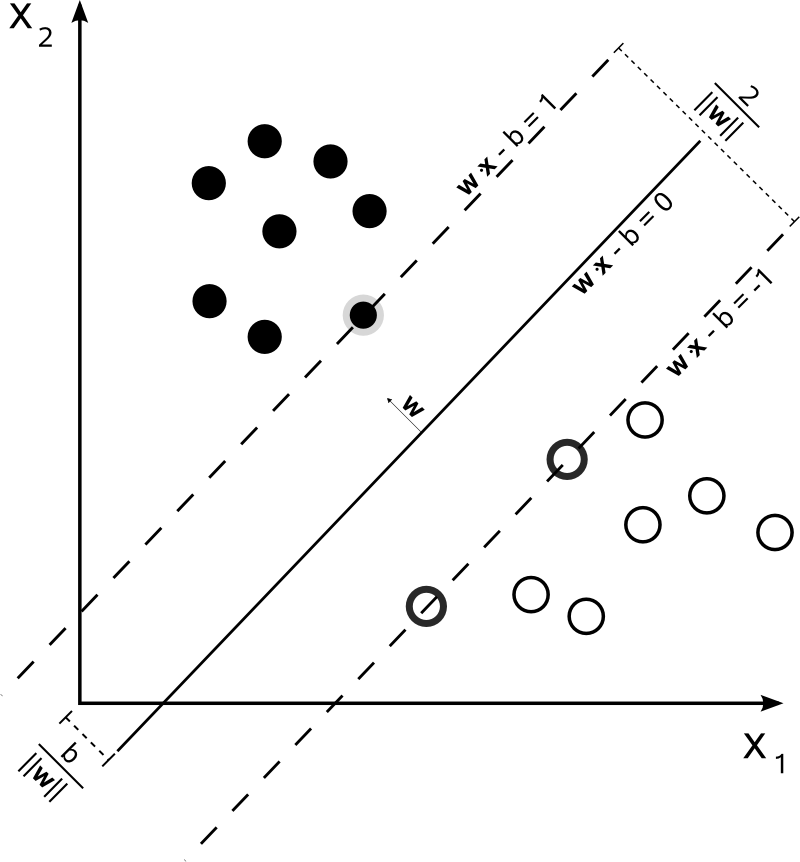
\includegraphics[scale = 0.3]{Svm_max_sep_hyperplane_with_margin.png}
\caption{SVM with maximum margin hyperplane (Source: Wikipedia)}
\label{fig:svm}
\end{center}
\end{figure}

In many applications, non-linear classifiers provide better accuracies than linear classifiers as they are able to discover better decision boundaries. But linear classifiers have advantages over non-linear classifiers as they often have simple training algorithms that scale well with the number of examples. \citep{VapnikSVMKernel:92} introduced the idea of kernels which use the machinery of linear classifiers to discover non-linear decision boundaries by fitting the maximum-margin hyperplane in a transformed feature space. Some common kernels include:
\begin{itemize}
\item Polynomial: $k(\bm{x_i},\bm{x_j}) = (\bm{x_i \cdot x_j})^d$
\item Gaussian Radial Basis Function: $k(\bm{x_i},\bm{x_j}) = exp(-\gamma||\bm{x_i - x_j}||^2)$
\end{itemize}
We experiment with the standard linear kernel and the RBF kernel.

\subsection{Feature Normalization}
Feature Normalization plays a very important role in many learning and optimization algorithms. In practice, many methods work best after the data has been normalized and whitened. Since Support Vector Machine algorithms are sensitive to scaling and have been shown to give better results with normalization, we experiment with two ideas - feature scaling and feature standardization:

\subsubsection{Feature Scaling}
One of the simplest methods to normalize features is to scale the ranges of features to a common range, [-1,1] in our case. The main advantage offered by scaling is that it avoids attributes in smaller numeric ranges being dominated by attributes in greater numeric ranges. It also avoids numerical difficulties like overflow errors caused by large attribute values. Note that both training and testing data should be scaled with the same parameters, otherwise the results would be erroneous. The transformation is obtained by:
\begin{equation}
\label{eq:FeatureScaling}
x' = minReqd + (maxReqd-minReqd)*\left(\frac{x-min}{max-min}\right)
\end{equation}

\subsubsection{Feature Standardization}
For a heterogeneous feature space, feature standardization makes the values of each feature in the data have zero-mean and unit-variance. The following transformation formula achieves the zero-mean and unit-variance requirements:
\begin{equation}
\label{eq:FeatureStandardization}
x' = \frac{x-\mu}{\sigma}
\end{equation}

The mean($\mu$) and variance($\sigma^2$) used in equation \ref{eq:FeatureStandardization} are the sample mean and unbiased sample variance, estimated from the training data. Note that the same transformation must be applied to train and test data to obtain meaningful results.

\section{Implementation}
In this section, we outline some of the important resources which have been used in the implementation: 
\begin{itemize}
\item Access to the WordNet graph was facilitated by extJWNL \footnote{\url{http://extjwnl.sourceforge.net/}}.

\item For WordNet based Word Similarity, we make use of Java WordNet::Similarity \footnote{\url{http://www.sussex.ac.uk/Users/drh21/}} by David Hope, which is a pure Java implementation of Ted Pedersen's Perl WordNet::Similarity \footnote{\url{http://wn-similarity.sourceforge.net/}}.

\item The BabelNet based features were obtained using the BabelNet API \citep{NavigliPonzetto:2012acl}.

\item To train the support vector machine classifier we used SVM implementation by \citep{Joachims98makinglarge-scale}, whose java access is provided by JNI-SVMLight \footnote{JNI-SVMLight: \url{http://adrem.ua.ac.be/~tmartin/}} library.

\item For Information Gain and Gain Ratio study in section \ref{section:InformationGainAndGainRatioStudy}, we use Weka software \citep{wekaSoftware}.
\end{itemize}

\section{Experimental Setup and Evaluation}
\label{section:SupervisedExperimentalSetupAndEvaluation}
\subsection{Train and Test datasets}
Since the quality assurance of Ontonotes dataset is reasonably high and no information is available about Senseval-2 dataset, we use binary classification dataset obtained from OntoNotes for training and validation. We split our dataset into a training set(70\%) and a held-out validation set(30\%). 
\begin{center}
\begin{longtable}{| l | l |}      
    \hline
    Examples & Nouns \\ \hline    
    Positive Examples\footnote{Pair of synsets merged by annotators} & 1214 \\ \hline
    Negative Examples\footnote{Pair of synsets not merged by annotators} & 11974 \\ \hline
    Percentage of Positive examples & 9.20 \\ \hline
    Positive Training examples in random 70\% sample & 850 \\ \hline
    Negative Training examples in random 70\% sample & 8382 \\ \hline
    Positive Testing examples in random 30\% sample & 364 \\ \hline
    Negative Testing examples in random 30\% sample & 3612 \\ \hline    
    \caption{Statistics of Pairwise Classification Dataset}
  \label{tab:pairwiseData}
\end{longtable}
\end{center}
\begin{comment}
\begin{center}
\begin{longtable}{| l | l | l |}      
    \hline
    Examples & Nouns & Verbs \\ \hline    
    Positive Examples\footnote{Pair of synsets merged by annotators} & 1214 & 6881 \\ \hline
    Negative Examples\footnote{Pair of synsets not merged by annotators} & 11974 & 20899 \\ \hline
    Percentage of Positive examples & 9.20 & 24.76 \\ \hline
    Positive Training examples in random 70\% sample & 850 & 4817\\ \hline
    Negative Training examples in random 70\% sample & 8382 & 14630\\ \hline
    Positive Testing examples in random 30\% sample & 364 & 2064\\ \hline
    Negative Testing examples in random 30\% sample & 3612 & 6269\\ \hline    
    \caption{Statistics of Pairwise Classification Dataset}
  \label{tab:pairwiseDataNounVerb}
\end{longtable}
\end{center}
\end{comment}

\subsection{Effect of class distribution in learning}
We trained two systems, which differ in number of negative examples used in training. One uses the whole 70\% dataset extracted and other selects random instances from negative examples of this dataset to get a balanced dataset (equal number of positive and negative instances). For testing, we again used a balanced dataset consisting of equal number of positive and negative instances, disjoint from the training dataset. The former classified all the instances into negative class. We attribute this to the skewed class distribution in the training data. On the other hand, we observe that system 2 learns better boundaries due to the balanced nature of the training set.

Owing to the above observations, for training as well as testing, we used randomly generated balanced datasets(equal number of positive and negative instances - 850 instances from each class) and repeated the process multiple number of times.

\subsection{Effect of normalization schemes and kernels}
\label{section:SVMNormalizationKernelExperiment}
It is known that large margin classifiers are sensitive towards feature scaling and standardization \citep{chang2011libsvm}. To study the same, we experiment with Attribute Normalization techniques and Kernel selection: Min-Max normalization and Z-Score normalization along with Linear and RBF Kernel. 

We perform 5-fold validation i.e. we train the SVM on 5 randomly generated balanced datasets and test them again on a randomly balanced dataset disjoint from the training set. The table \ref{tab:nounExp2} documents the average results of the 5 runs. We report only FScore over both the classes as a measure of performance of the systems. For detailed results of the experiments, refer Appendix \ref{appendix:SVMResults}.

\begin{center}
\begin{longtable}{| c | c | c | c |}      
\hline
Kernel & No Normalization & MinMaxNormalization & ZScoreNormalization\\ \hline
Linear & (0.31, 0.68) & (\textbf{0.73, 0.72}) & (0.05, 0.67)\\ \hline
RBF    & (0.70, 0.37) & (\textbf{0.73}, 0.70) & (0.64, \textbf{0.72})\\ \hline    
\caption{Studying Performance by varying Normalization Schemes and Kernels}
\label{tab:nounExp2}
\end{longtable}
\end{center}

For comparison purposes, we report the performance of the SVM systems, learnt for the 5-fold validation study (described above), on the Senseval-2 Dataset as the test set, in table \ref{tab:nounExp3}.

\begin{center}
\begin{longtable}{| c | c | c | c |}      
\hline
Kernel & No Normalization & MinMaxNormalization & ZScoreNormalization\\ \hline
Linear & (0.15, \textbf{0.90}) & (\textbf{0.44}, 0.81) & (0.01, \textbf{0.90})\\ \hline
RBF    & (0.37, 0.46) & (0.40, 0.69) & (0.41, 0.85)\\ \hline
\caption{SVM Performance on Senseval-2 Dataset}
\label{tab:nounExp3}
\end{longtable}
\end{center}

Observe that both feature normalization as well as kernel selection have a great influence on the classification performance. \citep{chang2011libsvm} report that if the data is not normalized the accuracy of an SVM can severely degrade. Therefore it is important to select the appropriate normalization and kernel for the task.   

For most of the normalization-kernel combinations, the performance is biased towards a particular class. Among the normalization techniques, MinMax Normalization seems to give consistently good performance in both the kernels. So for further studies, we decided to use MinMax Normalization on features. 

Linear Kernel gives better results on both the Senseval-2 dataset and the cross validation, and hence we choose linear kernel over RBF kernel.

\begin{comment}
For MinMax Normalization, the performance difference between linear and RBF kernel is not much. We select Linear kernel for further purposes as it is simpler (Occam's razor) ????
\end{comment}

\subsection{Feature Analysis}
We analyze our feature space in two ways. We evaluate Information Gain and Gain Ratio functions over the features and do a feature ablation study. The former tries to capture the discrimination ability of the feature by itself and the latter tries to measure how a feature corroborates with other features in the feature space.

\subsubsection{Information Gain and Gain Ratio Study}
\label{section:InformationGainAndGainRatioStudy}
\paragraph{Information Gain}
The Information Gain function is based on the notion of entropy, which characterizes the impurity of an arbitrary set of examples distributed among some classes. If an example is randomly selected from a set and its class $c_i$ is announced, then the probability of this announcement is equal to $p_i = \frac{|c_i|}{|D|}$ , and the amount of information it conveys is $-\log_2(p_i)$. The expected information provided by a announcement with respect to the class membership in a dataset $D$, having $m$ classes with estimated class probabilities $p_1,\ldots,p_m$, is given by:
\begin{equation}
Info(D) = -\sum_{i=1}^{m} p_i \log_2(p_i)
\end{equation}

The quantity $Info(D)$ measures the average amount of information(in bits) needed to identify the class of an example in $D$. We consider a similar measurement after $D$ has been partitioned on attribute $A$ in $v$ parts, labeled as $D_1,\ldots D_v$. The amount of information needed to arrive at an exact classification after partitioning using that attribute is the weighted sum over subsets and is given by:

\begin{equation}
Info_A(D) = \sum_{j=1}^v \frac{|D_j|}{|D|} \times Info(D_j)
\end{equation}

The Information Gain is the expected reduction of information requirements caused by knowing the value of $A$ and is given by:
\begin{equation}
Gain_A(D) = Info(D) - Info_A(D)
\end{equation}

\paragraph{Gain Ratio}
The Information Gain function is biased towards tests with many outcomes. To counter the same, Gain Ratio modifies the Information Gain by taking into account the number and sizes of the partitions obtained in a test.

The \textit{split information value} measures the potential information generated by dividing the dataset $D$ into $v$ bins, corresponding to $v$ outcomes on attribute $A$.

\begin{equation}
SplitInfo_A(D) = -\sum_{j=1}^{v}\frac{|D_j|}{|D|} \times \log_2\left(\frac{|D_j|}{|D|}\right)
\end{equation}

The gain ratio is defined as:

\begin{equation}
GainRatio_A(D) = \frac{Gain_A(D)}{SplitInfo_A(D)}
\end{equation}

\paragraph{Evaluation}
We computed all the features over the complete OntoNotes dataset without any normalization and evaluated the same using Information Gain and Gain Ratio as measures. Table \ref{tab:FeatureWiseEvaluation} compares the value for all the features. We highlight the top 7 features according to both the attribute evaluators.

\begin{center}
\begin{longtable}{| c | c | c |}      
\hline
\textbf{Feature} & \textbf{Gain Ratio} & \textbf{Information Gain} \\ \hline
LCH & 0.01288 & \textbf{0.0323} \\ \hline
WUP & 0.0148 & \textbf{0.02899} \\ \hline
JCN & \textbf{0.0215} & 0.02094 \\ \hline
LIN & 0.01943 & 0.02072 \\ \hline
RES & 0.01379 & 0.02335 \\ \hline
AdapLesk & 0.01688 & \textbf{0.03456} \\ \hline
AdapLeskTani & \textbf{0.02306} & \textbf{0.03603} \\ \hline
AdapLeskTaniNoHypo & 0.01685 & \textbf{0.03014} \\ \hline
\hline
Common Lemma Count & 0.00438 & 0.00394 \\ \hline
SenseCount & 0.00293 & 0.00293 \\ \hline
SenseNum & 0.0 & 0.0 \\ \hline
lexFileSimilarity & 0.01552 & 0.01143 \\ \hline
mergeSP1\_1 & 0.00282 & 0.00151 \\ \hline
mergeSP1\_2 & \textbf{0.04195} & 0.00103 \\ \hline
mergeSP1\_2\_relaxed & \textbf{0.04709} & 0.00119 \\ \hline
mergeSP1\_3 & 0.0 & 0.0 \\ \hline
number of Common Hypernyms & \textbf{0.08833} & 0.00965 \\ \hline
autohyponymy & 0.0 & 0.0 \\ \hline
\hline
Domain-Cosine Similarity & \textbf{0.01997} & \textbf{0.04416} \\ \hline
Domain-l1 Distance & 0.00445 & 0.00219 \\ \hline
Domain-l2 Distance & 0.00771 & 0.00238 \\ \hline
OEDMerged & \textbf{0.0326} & \textbf{0.03123} \\ \hline
SentiWordNet-CosineSimilarity & 0.0 & 0.0 \\ \hline
SentiWordNet-l1 Distance & 0.0 & 0.0 \\ \hline
SentiWordNet-l2 Distance & 0.0 & 0.0  \\ \hline
CommonEnglishTranslations & 0.00829 & 0.00671 \\ \hline
CommonGermanTranslations & 0.00732 & 0.00559 \\ \hline
CommonSpanishTranslations & 0.00547 & 0.00445 \\ \hline
CommonItalianTranslations & 0.00505 & 0.00418 \\ \hline
CommonFrenchTranslations & 0.00737 & 0.00634 \\ \hline
CommonCatalanTranslations & 0. 0.00657 & 0.00533 \\ \hline
CommonDBpediaEntries & 0.0 & 0.0 \\ \hline
\caption{Information Gain and Gain Ratio Based Evaluation}
\label{tab:FeatureWiseEvaluation}
\end{longtable}
\end{center}

\subsubsection{Feature Ablation Study}
We divide our features in 6 categories: WordNet Similarity measures, WordNet based features, eXtended WordNet Domains features, BabelNet features, SentiWordNet features and Navigli OED Mappings. 

We report the average F-Score of both the classes observed by removing that category of features from our feature space, retraining and retesting the classifiers on randomly generated balanced datasets, keeping everything else the same. The SVMs are trained using linear kernel and features are normalized using MinMax Normalization for all the experiments reported in this study. The table \ref{tab:nounEvalFeatureAblation} summarises the study.

\begin{center}
\begin{longtable}{| c | c | c |}  
\hline
\textbf{Features Removed} & \textbf{FScore Positive} & \textbf{FScore Negative} \\ \hline
WordNet Similarity Measures & 0.6948 & 0.6784 \\ \hline
WordNet Based Features & 0.7227 & 0.7092 \\ \hline
BabelNet Features & 0.7232 & 0.7127 \\ \hline
Domain Similarity Features & 0.6814 & 0.6619 \\ \hline
OED Feature & 0.6957 & 0.7212 \\ \hline
SentiWordNet Features & 0.7262 & 0.7192 \\ \hline
\hline
\textbf{Without Removing Features} & 0.7262 & 0.7192 \\ \hline
\caption{Feature Ablation Study}
\label{tab:nounEvalFeatureAblation}
\end{longtable}
\end{center}

\subsubsection{Observations}

\paragraph{WordNet Similarity Features}: 
The similarity measures have a significant effect on the performance of the SVMs as can be observed from table \ref{tab:nounEvalFeatureAblation}. This highlights the importance of the underlying ontology structure of the WordNet which these similarity measures try to capture.

Note from table \ref{tab:FeatureWiseEvaluation} that the gloss based features(the lesk variants - refer section \ref{section:similarityMeasures}) have high Information Gain values. This can be attributed to the fact that the annotators primarily rely on gloss descriptions to interpret synsets. In the relatedness study by \citep{mccarthy2006relating}, the annotators only had glosses as evidence to decide if senses were ``related'' or not.

\paragraph{WordNet Based Features}:
Among the WordNet based features, the features relating the synsets to their hypernyms like the ``SP1\_2 merge heuristics'', the number of common hypernyms etc. seem to be discriminatory. This is understandable as the hypernym related feaures capture the notion of semantic generalization, which is essential to undestand a sense. 

\paragraph{BabelNet Features}:
The objective of using multilingual features was to test whether the translation equivalences are powerful enough to capture semantic associations between two word senses. Low values of the Information Gain and Gain Ratio of the BabelNet features reflect that the above heuristic is a weak indicator for sense-merging. 

Using mapping to DBPedia entries as a feature was an effort to harness the DBpedia Knowledge Base \footnote{\url{http://dbpedia.org/About}}. But we observe from table \ref{tab:FeatureWiseEvaluation} that the feature is not that useful. A better use of the DBpedia ontology would be to estimate the similarity of mapped concepts using the underlying hierarchy.

\paragraph{Domain Similarity Features}:
Intuitively, as an annotator, approximately matching the domain of two senses serves as a strong cue about whether the two senses are semantically related enough to be merged. This is justified by the high info-gain and gain-ratio values for the domain similarity features.

\paragraph{Oxford English Dictionary Mapping}:
\citep{Navigli06meaningfulclustering} have already shown the effectiveness of this mapping in a WSD task based setting. High values of Information Gain and Gain Ratio support the same. The problem we face with the feature is its incompleteness as not all the word senses are clustered by mapping to Oxford English Dictionary.

\paragraph{SentiWordNet Features}: 
Another interesting set of features is the SentiWordNet based features. Their removal doesn't affect the system's performance which can be attibuted to the fact that most of the noun synsets in the SentiWordNet project are described as objective concepts. Their non-discriminatory nature is substantiated by the Information Gain and Gain Ratio based study as well (refer table \ref{tab:FeatureWiseEvaluation}). 

\section{Discussion}
In this section, we would like to address some concerns regarding the similarity function learnt.

\subsection{Inconsistent Predictions} 
\label{section:SVMInconsistentPredictions}
Using the outputs of the SVM learnt directly as the similarity distance poses the problem of inconsistent predictions i.e. it can happen that for three synsets $A$, $B$ and $C$, $sim_{SVM}(A,B) > 0$ and $sim_{SVM}(B,C) > 0$ while $sim_{SVM}(A,C) < 0$. Such inconsistencies, though rare, can happen. Even the human annotators involved in preparation of Senseval-2 dataset \citep{Senseval2LexicalSampleTask} have made such errors. This motivates us to utilize the WordNet structure to correct such inconsistencies. % I can give exact number here !

\subsection{Coverage of the SVM} 
The training data for the SVM is not representative of the WordNet synsets because we trained only on the synset pairs that have atleast one lemma in common. It is interesting to note here that the number of synsets which contain atleast one polysemous lemma is only 33155 out of total 82115 synsets. This questions the idea of using the SVM models learnt as generic synset similarity estimators. 

\citep{snow07mergesense} addresses this issue by taking similarity between synsets not sharing any word as $0$ and for the synsets sharing atleast a word as the prediction by the SVM, for the purpose of sense-merging. Because of the heterogeneous nature of the similarity defined by \citep{snow07mergesense}, it does not serve as a generic synset similarity measure.

\subsection{Insufficient Data for Learning}
The SVMs were learnt on randomly selected balanced datasets of 1700 instances with 850 instances of each class. Though the results are promising, the number of training instances is small as compared to the total number of synsets involved (33155), which makes it tough to judge whether the similarity metric learnt is generic enough or not.

\section{Conclusions and Future Work}
\citep{mccarthy2006relating} performed an annotation study in which 3 native english speakers were asked to label around 300 sense pairs as ``related'', ``unrelated'' or ``don't know''. The inter-annotator F-Scores were (0.7926, 0.5454, 0.4874)\footnote{Since the annotation was done by native speakers and not experienced linguists or lexicographers, we can expect a slightly higher inter-annotator F-Score for the task.} \citep{mccarthy2006relating} \citep{snow07mergesense}. These figures highlight that humans differ in their tendency to split or lump senses and that the task is inherently a difficult one.

Significant advancement of supervised learning algorithms over the last two decades and their ability to capture the relative importance of features essential to the task in hand inspired us to utilize their potential in understanding the importance of the various features in merging synsets.

The use of external corpora for supervision is motivated by the fact that we are not able to fully capture the information in WordNet for e.g. we are not able to utilize the gloss of the synset beyond lexical measures. By enriching the semantic information of the synsets using features like belongingness to different domains, sentiment associated with them etc. we are able to improve the performance of our systems. 

The evaluation suggests that there is a need to enrich WordNet along with the production of additional resources to better understand word senses. Some such efforts include augmenting WordNet with teleological links \footnote{\url{http://wordnetcode.princeton.edu/standoff-files/teleological-links.xls}}, morphological and semantic information \citep{morphosemanticLinks}. 
	%\chapter{Semi-Supervised Synset Similarity}
\label{chapter:Semi-SupervisedSynsetSimilarity}
In this chapter, we describe the idea of SimRank, its personalization and application to learning synset similarity in a semi-supervised fashion. Further we discuss how to coarsen the WordNet taxonomy and evaluate the clustering obtained in a WSD task based setting.

\section{Motivation}
The small coverage of the Support Vector Machines that we saw in section \ref{sec:supervisedAlgoOutline} makes them unsuitable to be used as a generic synset similarity estimator. To learn the similarity between synsets which do not share a word, we wish to utilize the relations encoded in WordNet as well as the information learnt using supervision. 
The ability of the Personalized SimRank framework to propogate the seeded information using semantic links between concepts allows us to learn complete synset similarity estimates.

\section{SimRank}
\label{sec:SimRank}
\subsection{Introduction}
SimRank \citep{Jeh02simrank} is a graph based similarity measure applicable in any domain with object-to-object relationships, with intuition that ``\textbf{two objects are similar if they are referenced by similar objects}'' \citep{Jeh02simrank} \citep{LizorkinSimrank}. Since SimRank has a recursive intuition, the base cases play an important role here.

Before discussing the model, let us introduce some notation for convenience. For a graph $G(V,E)$, for each node $v \in V$, we define the following:
\begin{itemize}
\item $I(v)$ is a set consisting of in-neighbours of node $v$ i.e.
\begin{equation}
I(v) = \{w\in V | (w,v)\in E\}
\end{equation}
\item $O(v)$ is a set consisting of out-neighbours of node $v$ i.e.
\begin{equation}
O(v) = \{u\in V | (v,u)\in E\}
\end{equation}
\end{itemize}

Individual members of $O(v)$ and $I(v)$ are referred to as $O_i(v)$, $1\leq i \leq |O(v)|$ and $I_j(v)$, $1\leq j \leq |I(v)|$.

Let $s(\alpha,\beta)$ denote the similarity score between objects $\alpha$ and $\beta$. The SimRank equation is given by: 
\begin{equation} \label{eq:SimRankBasic}
s(\alpha,\beta) =
\left\{ \begin{array}{rl}
1 & \mbox{if } \alpha=\beta \\
0 &  \mbox{ if } I(\alpha)=\phi \mbox{ or } I(\beta)=\phi \\
\frac{C}{|I(\alpha)||I(\beta)|}\sum_{i=1}^{|I(\alpha)|}\sum_{j=1}^{|I(\beta)|} s(I_i(\alpha),I_j(\beta)) & \mbox{ otherwise } \\
\end{array}\right.
\end{equation}
Here $C$ is a constant in range $(0,1)$ and is called the decay factor.

\subsection{Solution and its Properties}
\label{section:SimRankSolutionsAndProperties}
The solution to the SimRank equation \ref{eq:SimRankBasic} for a graph $G(V,E)$ is reached by iteration to a fixed-point. For each iteration $k$, we keep ${|V|}^2$ entries $S_k(\ast,\ast)$, where $S_k(\alpha,\beta)$ is the estimate of similarity between $\alpha$ and $\beta$ on $k^{th}$ iteration.
We start with $S_0(\ast,\ast)$ which is $1$ for singleton nodes like $(x,x)$, $0$ otherwise.

We successively compute $S_{k+1}(\ast,\ast)$ based on $S_k(\ast,\ast)$:
\begin{equation} \label{eq:SimRankBasicRecursive}
S_{k+1}(\alpha,\beta) =
\left\{ \begin{array}{rl}
1 & \mbox{if } \alpha=\beta \\
0 &  \mbox{if } I(\alpha)=\phi \mbox{ or } I(\beta)=\phi \\
\frac{C}{|I(\alpha)||I(\beta)|}\sum_{i=1}^{|I(\alpha)|}\sum_{j=1}^{|I(\beta)|} S_k(I_i(\alpha),I_j(\beta)) & \mbox{otherwise } \\
\end{array}\right.
\end{equation}

Let us highlight some properties of SimRank covered in \citep{Jeh02simrank} and \citep{LizorkinSimrank}:
\begin{enumerate}
\item A solution $s(\ast,\ast)$ to SimRank equations always exist and is unique, and $s(\ast,\ast) \in [0,1]$
\item For each $k$, $S_k(\ast,\ast)$ is upper bounded by the SimRank function $s(\ast,\ast)$ i.e.
\begin{equation}
 S_k(\alpha,\beta) \leq s(\alpha,\beta)
\end{equation}
\item Iterative functions $S_k(\ast,\ast)$ converge to SimRank function $s(\ast,\ast)$ i.e. 
\begin{equation}
\displaystyle \lim_{k \rightarrow \infty}S_k(\alpha,\beta)=s(\alpha,\beta)
\end{equation}
\item The difference between the SimRank scores and iterative similarity scores decreases exponentially in the number of iterations and uniformly for every pair of nodes i.e. 
\begin{equation} \label{SimRankExponentialConvergence}
s(\alpha,\beta) - S_k(\alpha,\beta) \leq C^{k+1} \mbox{\ \ \ \ }\forall \alpha,\beta \in V;\mbox{  } k=0,1,2\ldots
\end{equation}
\end{enumerate}

\subsection{Random Surfer Pair Model}
\citep{Jeh02simrank} show that the SimRank similarity score $s(\alpha,\beta)$ measures how soon two random surfers are expected to meet at the same node if they start at nodes $\alpha$ and $\beta$ and randomly walk the graph backwards.

\begin{equation}
s(\alpha,\beta) = \sum_{t:(\alpha,\beta) \rightsquigarrow (x,x)} P[t]C^{l(t)}  \label{eq:emd} 
\end{equation}

More formally, $s(\alpha,\beta)$ is the \textit{expected f-meeting distance} traveling back edges, between the nodes $\alpha$ and $\beta$ with $f(z)=C^z$.

\section{Personalized Weighted SimRank}
\subsection{Weighted SimRank}
Many times while working with real data, we observe relationships of different types between objects, which are likely to have different weights associated with them. For learning similarity between objects having such underlying structure, we discuss a weighted version of the SimRank method proposed in \citep{Jeh02simrank} and discussed in section \ref{sec:SimRank}. For convenience, let us define $W_{I}(n)$ and $W_{O}(n)$, for a node $n$ as follows:
\begin{align}
W_{O}(n) &= \sum_{i=1}^{|O(n)|} w(n,O_i(n)) \\
W_{I}(n) &= \sum_{i=1}^{|I(n)|} w(I_i(n),n)
\end{align}

The recursive equation for weighted SimRank is as follows:
\begin{align}
s(\alpha,\beta) = \frac{C}{W_{I}(\alpha)W_{I}(\beta)} \sum_{i=1}^{|I(\alpha)|} \sum_{j=1}^{|I(\beta)|} w(I_i(\alpha),\alpha) \cdot w(I_j(\beta),\beta) \cdot s(I_i(\alpha),I_j(\beta)) \label{eq:SimRankWeighted}
\end{align}

\noindent
The relation \ref{eq:SimRankWeighted} is obtained by extending the Random Surfer Pairs Model of SimRank and is discussed in more detail in Appendix \ref{appendix:weightedSimRank}.

\subsection{Personalizing SimRank}
\label{subsection:PersonalizedSimRank}
In many scenarios, while working with objects, we don't have complete information about the objects and thus have similarities for only some pair of objects. These similarities may be independently learnt and may not directly conform with the underlying graph. In such situations, we would like to get a more complete and consistent similarity metric between objects but we would like to use the information given to us as well. For the same, we propose a personalized framework for SimRank, in which we bias the SimRank by changing the initialization.
If we know similarities of some pairs, we fix them in our set of equations and let the rest of the values be automatically learned by the system.

Lets call the map of node pairs to their similarity values as $InitStore$. All the singleton nodes like $(x,x)$ have value equal to 1. The system of equations is defined as follows: 

\begin{equation} \label{eq:PersonalizedWeightedSimRank}
{\footnotesize
s(\alpha,\beta) =
\left\{ \begin{array}{rl}
1 & \mbox{if } \alpha=\beta\\
InitStore[(\alpha,\beta)] & \mbox{if } (\alpha,\beta) \in InitStore\\
\frac{C}{W_{I}(\alpha)W_{I}(\beta)} \sum_{i=1}^{|I(\alpha)|} \sum_{j=1}^{|I(\beta)|} w(I_i(\alpha),\alpha) \cdot w(I_j(\beta),\beta) \cdot s(I_i(\alpha),I_j(\beta)) & \mbox{otherwise }
\end{array}\right.
}
\end{equation}
In the personalized framework, we have no constraints over the initialization as long as all values initialized are in range $[0,C]$. 

\subsection{Solution of Personalized SimRank}
\label{section:ComputingPersonalizedSimRank}
A solution to the equations \ref{eq:PersonalizedWeightedSimRank} for a graph $G(V,E)$ is computed on lines of the method to solve equation \ref{eq:SimRankBasic} (refer section \ref{section:SimRankSolutionsAndProperties}). The successive computation of $S_{k+1}(\ast,\ast)$ from $S_k(\ast,\ast)$ is calculated as follows:
\begin{equation} \label{eq:PersonalizedWeightedSimRankSolution}
{\footnotesize
S_{k+1}(\alpha,\beta) =
\left\{ \begin{array}{rl}
1 & \mbox{if } \alpha=\beta\\
InitStore[(\alpha,\beta)] & \mbox{if } (\alpha,\beta) \in InitStore\\
\frac{C}{W_{I}(\alpha)W_{I}(\beta)} \sum_{i=1}^{|I(\alpha)|} \sum_{j=1}^{|I(\beta)|} w(I_i(\alpha),\alpha) \cdot w(I_j(\beta),\beta) \cdot S_k(I_i(\alpha),I_j(\beta)) & \mbox{otherwise}
\end{array}\right.
}
\end{equation}

All the properties of solution to SimRank equation are applicable to Personalized SimRank solution as well (refer section \ref{section:SimRankSolutionsAndProperties}). We prove all these properties for Personalized SimRank in Appendix \ref{appendix:PersonalizedSimRankProperties}.

\section{Personalized SimRank for Learning Synset Similarity}
\label{section:PersonalizedSimRankForLearningSynsetSimilarity}

%treating WordNet synsets as concepts

\subsection{Algorithm Outline}
\label{section:semiSupervisedAlgoOutline}
The Personalized SimRank framework requires an underlying graph $G(V,E)$, where $V$ is the set of objects to be clustered and $E$ is the set of semantic links connecting these objects and an $InitStore$ which contains the similarity values over some pairs from $V\times V$ learnt or known beforehand. Note that the values in the $InitStore$ have an upper bound of $C$.

For learning synset similarity, $V$ is the set of synsets to be clustered and $E$ is the set of WordNet relations connecting these synsets. We use the \textit{Hypernymy}, \textit{Hyponymy}, \textit{Meronymy} and \textit{Holonymy} relations of WordNet as the semantic links. We seed the $InitStore$ as follows:
\begin{itemize}
\item We predict the similarity values of all the synset pairs which share at least one word using the Support Vector Machine learnt from synset-merging data from OntoNotes \citep{Hovy:2006} as described in section \ref{sec:ClassifierAndTraining}.
\item We transform the SVM predictions to the range $[0,1]$ using the sigmoid model learnt on the OntoNotes dataset. (see section \ref{sec:EstimatingPosteriorProbabilitiesFromSVMScores})
\item We scale the posterior probabilities obtained to range between $[0,C]$ by linear scaling, where $C$ is the SimRank decay parameter.
\end{itemize}

\subsection{Estimating Posterior Probabilities from SVM Scores}
\label{sec:EstimatingPosteriorProbabilitiesFromSVMScores}
Given a set of training examples $x_i \in \mathbb{R}^n, i=1,\ldots,t,$ labeled by $y_i \in \{-1,+1\}$ with $N_+$ positive examples and $N_-$ negative examples, a Support Vector Machine finds a maximum margin decision boundary $f(x)$ whose sign serves as a label prediction for any test example $x$. Instead of label prediction, many systems, as in our case: SimRank Initialization, require posterior probability $Pr(y= +1|x)$ estimate. 
\citep{Platt99} proposed approximating the posterior by a sigmoid function
\begin{align}
Pr(y=+1|x) \approx P_{A,B}(f(x)) \equiv \frac{1}{1+exp{(Af(x)+B)}}
\end{align}

To avoid overfitting of the sigmoid, an out-of-sample model is used i.e. for each training example target values $t_i$s are used (instead of 1 and 0), where 
\begin{equation} \label{eq:SVMTargetValues}
t_i =
\left\{ \begin{array}{rl}
\frac{N_+ +1}{N_+ +2} & \mbox{if } y_i = +1\\
\frac{1}{N_- +2} & \mbox{if } y_i = -1\\
\end{array}\right.
\end{equation}

Let each $f_i$ be shorthand for $f(x_i)$. 
The best parameter setting $z^{\ast} = (A^{\ast},B^{\ast})$ is determined by solving the following regularized maximum likelihood problem:
\begin{align} \label{eq:regularizedMLProblem}
\displaystyle \min_{z=(A,B)} F(z) = - \sum_{i=1}^{t}\left( t_i \log(P_{A,B}(f_i)) + (1-t_i)\log(1-P_{A,B}(f_i))\right)
\end{align}

\citep{Platt99} indicated that for solving equation \ref{eq:regularizedMLProblem}, any method for unconstrained optimization can be used. We use Newton's method with backtracking, as proposed in \citep{Lin03Note}, as it avoids numerical difficulties faced by \citep{Platt99}. The pseudocode for the implementation is available in Appendix \ref{appendix:SVMProb}.

\subsection{Importance of Parameter \texorpdfstring{$C$}{TEXT} }
The parameter $C$ in Personalized SimRank affects the algorithm in many ways:
\begin{itemize}
\item \textbf{Maximum Similarity between distinct objects}: According to the SimRank equations, the maximum similarity between two distinct objects can be at most $C$.

\begin{align}
s(a,b) &= \frac{C}{W_{I}(a)W_{I}(b)} \sum_{i=1}^{|I(a)|} \sum_{j=1}^{|I(b)|} w(I_i(a),a)  \cdot w(I_j(b),b) \cdot \underbrace{s(I_i(a),I_j(b))}_{\leq 1}\\
&\leq \frac{C}{W_{I}(a)W_{I}(b)} \sum_{i=1}^{|I(a)|} \sum_{j=1}^{|I(b)|} w(I_i(a),a)  \cdot w(I_j(b),b)\\
&\leq \frac{C}{W_{I}(a)W_{I}(b)} \left( \sum_{i=1}^{|I(a)|} w(I_i(a),a) \right )  \cdot \left( \sum_{j=1}^{|I(b)|}  w(I_j(b),b) \right )\\
&\leq C
\end{align}

\item \textbf{Rate of convergence}: The rate of convergence of the iterative method to find the solution for SimRank equations is dependent on $C$ as there is exponential decrease in the difference between SimRank theoretical and iterative similarity scores in the number of iterations. In short, the higher the value of $C$, the slower is the convergence.
\end{itemize}

To understand the importance of the parameter $C$, we vary the value of $C$ in our experiments and empirically study the results obtained.

\section{Coarsening WordNet}
In this section we would discuss our method to cluster synsets of WordNet, which would give us coarser senses for words. The task in hand can be described as follows: Assuming we have a similarity metric which gives us similarity between each pair of synsets, we need to cluster the synsets where the granularity of the clustering can be adjusted according to the needs of the application.

We use the similarity metric learnt using the personalized SimRank model as described in section \ref{section:PersonalizedSimRankForLearningSynsetSimilarity}.
We construct a graph $G(V,E)$ where the vertices $V$ are the synsets of the WordNet graph and edges $E$ are obtained by thresholding the similarity metric.
On this graph, we find connected components, which gives us a partition over synsets.
The algorithm \ref{alg:CoarseningWordNet} summarises our method:

\begin{algorithm}[h]
\begin{algorithmic}[1]
 \State \textbf{Input: } WordNet Graph $WN(V,E)$, Similarity Metric $Sim$ and threshold $t$
 \State \textbf{Output: } Partition over $V$ 
 \State $E' \gets \emptyset$
 \ForAll{Synset $s_i \in V$}
  \ForAll{Synset $s_j \in V$}
    \If{$Sim(s_i,s_j) \geq t$} 
    $E' \gets E' \cup (s_i,s_j)$
    \EndIf
  \EndFor
 \EndFor 
 \State $C \gets ConnectedComponents(G(V,E'))$\\
 \Return $C$
\end{algorithmic}
\caption{Coarsening WordNet}
\label{alg:CoarseningWordNet}
\end{algorithm}

We use the clustering obtained to derive coarse senses of words. For a word, all its senses in the same cluster are merged and act as a coarse sense. Algorithm \ref{alg:QueryingSenses} summarises the querying method:

\begin{algorithm}[h]
\begin{algorithmic}[1]
 \State \textbf{Input: } WordNet Graph $WN(V,E)$, Word $w$ and Partition $P$ over $V$ 
 \State \textbf{Output: } Set of coarse senses $C$
 \State $L \gets ListSenses_{WN}(w)$
 \State $C \gets \emptyset$
 \ForAll{Synset $s_i \in L$}
  \State $C \gets C \cup \{s_i\}$
 \EndFor 
 \ForAll{Synset $s_i \in L$}
  \ForAll{Synset $s_j \in L$}
    \If{$s_i \neq s_j$ and $P(s_i,s_j) == 1$} 
    $C \gets Merge(C,s_i,s_j)$
    \EndIf
  \EndFor
 \EndFor  \\
\Return $C$
\end{algorithmic}
\caption{Querying Senses of a word}
\label{alg:QueryingSenses}
\end{algorithm}

\section{Experimental Setup and Evaluation}
\label{section:evaluation}
\subsection{Estimating Posterior Probabilities from SVM Scores}
We learn the parameters $A$ and $B$ of the sigmoid transforming SVM predictions to posterior probabilities (see section \ref{sec:EstimatingPosteriorProbabilitiesFromSVMScores}). Using the same data set that was used to train the model we want to calibrate will introduce unwanted bias. So we used an independent calibration set in order to get good posterior probabilities \citep{Niculescu-Mizil:2005}.

We address this problem by calibrating on an independently generated random balanced subsets from OntoNotes (see section \ref{sec:OntoNotesDataset}). The SVM predictions are obtained using the SVMs trained over random subsets of the OntoNotes data (see section \ref{section:SupervisedExperimentalSetupAndEvaluation}). Since all the SVMs were trained on randomly generated datasets, we selected the SVM that performed the best in cross validation.

The values of $A$ and $B$ obtained are -1.1655 and 0.0222 respectively. Using these values, the SVM prediction of value 0 gets mapped to 0.4944. 

\subsection{Semi-Supervised Similarity Learning}
We learn similarity models using the SimRank variant described in section \ref{section:semiSupervisedAlgoOutline}. \citep{Jeh02simrank} use $C=0.8$ and report that 5-6 iterations are enough. \citep{LizorkinSimrank} suggest to use lower values of $C$ or more number of iterations. We vary the values taken by $C$ as 0.6, 0.7 and 0.8. We run all the systems for 10 iterations to avoid convergence issues. 

We use the \textit{Hypernymy}, \textit{Hyponymy}, \textit{Meronymy} and \textit{Holonymy} relations of WordNet as the semantic links. All the semantic links used in all the experiments have uniform weight unity. For implementation, we used EZGraph Java library\footnote{ezgraph - Easy to Use Graph Analysis Library:  \url{https://code.google.com/p/ezgraph/}}.

\subsection{Coarsening WordNet}
We assess the effect of automatic synset clustering on the English all-words task at Senseval-3 \citep{Senseval3AllWordsTask} (this evaluation is similar to the evaluation used by \citep{Navigli06meaningfulclustering} and \citep{snow07mergesense}). The task asked WSD systems to select the apt sense for 2,041 content words in running texts comprising of 351 sentences. Since we focus on nouns, we used the 890 instances labelled with noun as the part of speech.

We consider the three best performing WSD systems: GAMBL \citep{decadt-EtAl:2004:Senseval-3}, SenseLearner \citep{mihalcea-faruque:2004:Senseval-3} and Koc University \citep{yuret:2004:Senseval-3} - and the best unsupervised system: IRST-DDD \citep{strapparava-gliozzo-giuliano:2004:Senseval-3} submitted in the task. The answer by the system is given full credit if it belongs to the cluster of the correct answer.

Observe that any clustering will only improve the WSD performance. Therefore to assess the improvement obtained because of our particular clustering, we calculate the expected performance for a random clustering at the same granularity as our clustering and study the improvement over random clustering instead. 

Score for a random clustering is calculated as follows: Let the word to be disambiguated have $N$ senses, each mapped to a unique synset. Let the clustering of these $N$ synsets on a particular granularity give us $k$ clusters $C_1,\ldots C_k$. The expectation that an incorrectly chosen sense and the actual correct sense would be in cluster $C_i$  in this clustering is $\frac{|C_i|(|C_i|-1)}{N(N-1)}$. Using linearity of expectation, we can say that the chances of the two synsets belonging to same cluster would be 
\begin{equation}
\frac{\sum_{i=1}^{k} |C_i|(|C_i|-1) }{N(N-1)}
\end{equation}

We experiment with $C$ = 0.6, 0.7 and 0.8. The SVM probability boundaries when scaled to $[0,C]$ for these values are 0.30, 0.35 and 0.40. So for finding the threshold giving the best improvement against random clustering baseline, we use the search space $[C-0.35, C]$. The performance of the systems at these thresholds for different values of $C$ is reported in %tables \ref{tab:wsdImprovement0.6}, \ref{tab:wsdImprovement0.7} and \ref{tab:wsdImprovement0.8}.
table \ref{tab:wsdImprovement}.

% \begin{center}
% \begin{longtable}{| c || c | c | c | c | c |}      
%     \hline
%     System & F-Score & Threshold & CCC & Random & Improvement \\ \hline
%     GAMBL & 0.7116 & 0.36 & 0.9031 & 0.8424 & 0.0607 \\ \hline
%     SenseLearner & 0.7104 & 0.37 & 0.8824 & 0.8305 & 0.0518 \\ \hline
%     KOC University & 0.7191 & 0.37 & 0.8924 & 0.8314 & 0.0610 \\ \hline
%     IRST-DDD & 0.6367 & 0.35 & 0.8731 & 0.8013 & 0.0718 \\ \hline
%     \caption{Improvement in Senseval-3 WSD performance using Connected Component Clustering Vs Random Clustering at the same granularity with C = 0.6}
%   \label{tab:wsdImprovement0.6}
% \end{longtable}
% \end{center}
% 
% \begin{center}
% \begin{longtable}{| c || c | c | c | c | c |}      
%     \hline
%     System & F-Score & Threshold & CCC & Random & Improvement \\ \hline
%     GAMBL & 0.7116 & 0.52 & 0.8453 & 0.7864 & 0.0589 \\ \hline
%     SenseLearner & 0.7104 & 0.49 & 0.8541 & 0.8097 & 0.0444 \\ \hline
%     KOC University & 0.7191 & 0.52 & 0.8448 & 0.7911 & 0.0538 \\ \hline
%     IRST-DDD & 0.6367 & 0.49 & 0.7970 & 0.7402 & 0.0568 \\ \hline
%     \caption{Improvement in Senseval-3 WSD performance using Connected Component Clustering Vs Random Clustering at the same granularity with C = 0.7}
%   \label{tab:wsdImprovement0.7}
% \end{longtable}
% \end{center}
% 
% \begin{center}
% \begin{longtable}{| c || c | c | c | c | c |}      
%     \hline
%     System & F-Score & Threshold & CCC & Random & Improvement \\ \hline
%     GAMBL & 0.7116 & 0.59 & 0.8419 & 0.7843 & 0.0577 \\ \hline
%     SenseLearner & 0.7104 & 0.56 & 0.8439 & 0.7984 & 0.0455 \\ \hline
%     KOC University & 0.7191 & 0.59 & 0.8414 & 0.7879 & 0.0535 \\ \hline
%     IRST-DDD & 0.6367 & 0.47& 0.8881 & 0.8324 & 0.0557 \\ \hline
%     \caption{Improvement in Senseval-3 WSD performance using Connected Component Clustering Vs Random Clustering at the same granularity with C = 0.8}
%   \label{tab:wsdImprovement0.8}
% \end{longtable}
% \end{center}

%%%%%%%%%%%%%%%%%%%%%%%%%%%%

\begin{center}
\begin{longtable}{|c| c || c | c | c | c | c |}      
    \hline
    C & \textbf{System} & \textbf{F-Score} & \textbf{Threshold} & \textbf{CCC} & \textbf{Random} & \textbf{Improvement} \\ \hline
    \multirow{4}{*}{0.6} & GAMBL & 0.7116 & 0.36 & 0.9031 & 0.8424 & 0.0607 \\ \cline{2-7}
    & SenseLearner & 0.7104 & 0.37 & 0.8824 & 0.8305 & 0.0518 \\ \cline{2-7}
    & KOC University & 0.7191 & 0.37 & 0.8924 & 0.8314 & 0.0610 \\ \cline{2-7}
    & IRST-DDD & 0.6367 & 0.35 & 0.8731 & 0.8013 & 0.0718 \\ \cline{2-7}
    \hline    
    \multirow{4}{*}{0.7} & GAMBL & 0.7116 & 0.52 & 0.8453 & 0.7864 & 0.0589 \\ \cline{2-7}
    & SenseLearner & 0.7104 & 0.49 & 0.8541 & 0.8097 & 0.0444 \\ \cline{2-7}
    & KOC University & 0.7191 & 0.52 & 0.8448 & 0.7911 & 0.0538 \\ \cline{2-7}
    & IRST-DDD & 0.6367 & 0.49 & 0.7970 & 0.7402 & 0.0568 \\ \cline{2-7}
    \hline    
    \multirow{4}{*}{0.8} &GAMBL & 0.7116 & 0.59 & 0.8419 & 0.7843 & 0.0577 \\ \cline{2-7}
    & SenseLearner & 0.7104 & 0.56 & 0.8439 & 0.7984 & 0.0455 \\ \cline{2-7}
    & KOC University & 0.7191 & 0.59 & 0.8414 & 0.7879 & 0.0535 \\ \cline{2-7}
    & IRST-DDD & 0.6367 & 0.47& 0.8881 & 0.8324 & 0.0557 \\
    \hline
    \caption{Improvement in Senseval-3 WSD performance using Connected Component Clustering Vs Random Clustering at the same granularity}
  \label{tab:wsdImprovement}
\end{longtable}
\end{center}

Commenting theoretically about the impact of $C$ on the performance is tough as by changing $C$ we are changing all the ${|V|}^2$ simultaneous equations to be solved. Empirically we observe that improvements over baseline keep on decreasing on increasing $C$ across all the systems. It might be because of the slow convergence of SimRank for higher values of $C$.

We observe from the figures \ref{fig:supervisedSystemsImprovement} and \ref{fig:unsupervisedSystemsImprovement} that by varying thresholds, the improvement of the Connected Components Clustering over the random clustering baseline at the same granularity first increases and then decreases.

Across supervised and unsupervised systems, we observe that the unsupervised systems obtain higher improvements than the supervised systems which can be attributed to fact that the unsupervised system used was underperforming compared to the supervised systems in the fine grained WSD task setting.

\begin{figure}
\centering
\subfigure[]{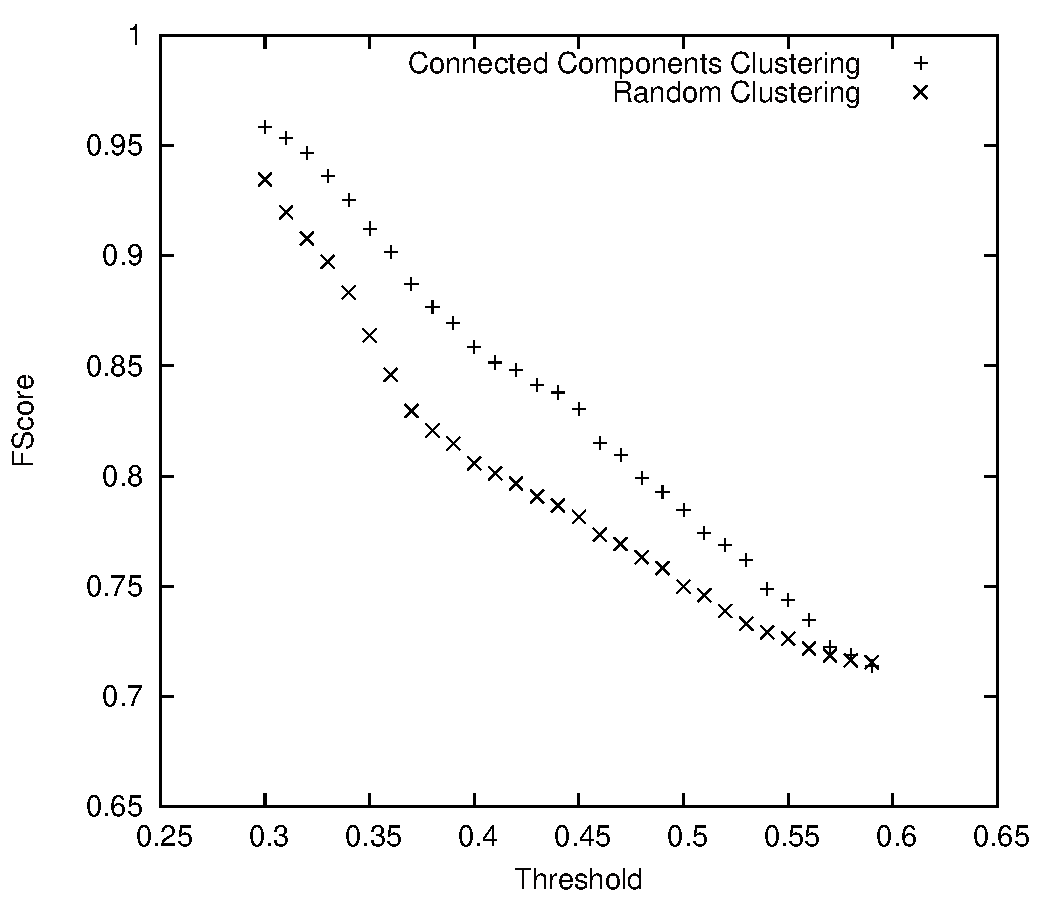
\includegraphics[width=2.9in]{SVMScaledSupervised6.pdf}\label{superviseda}}
\subfigure[]{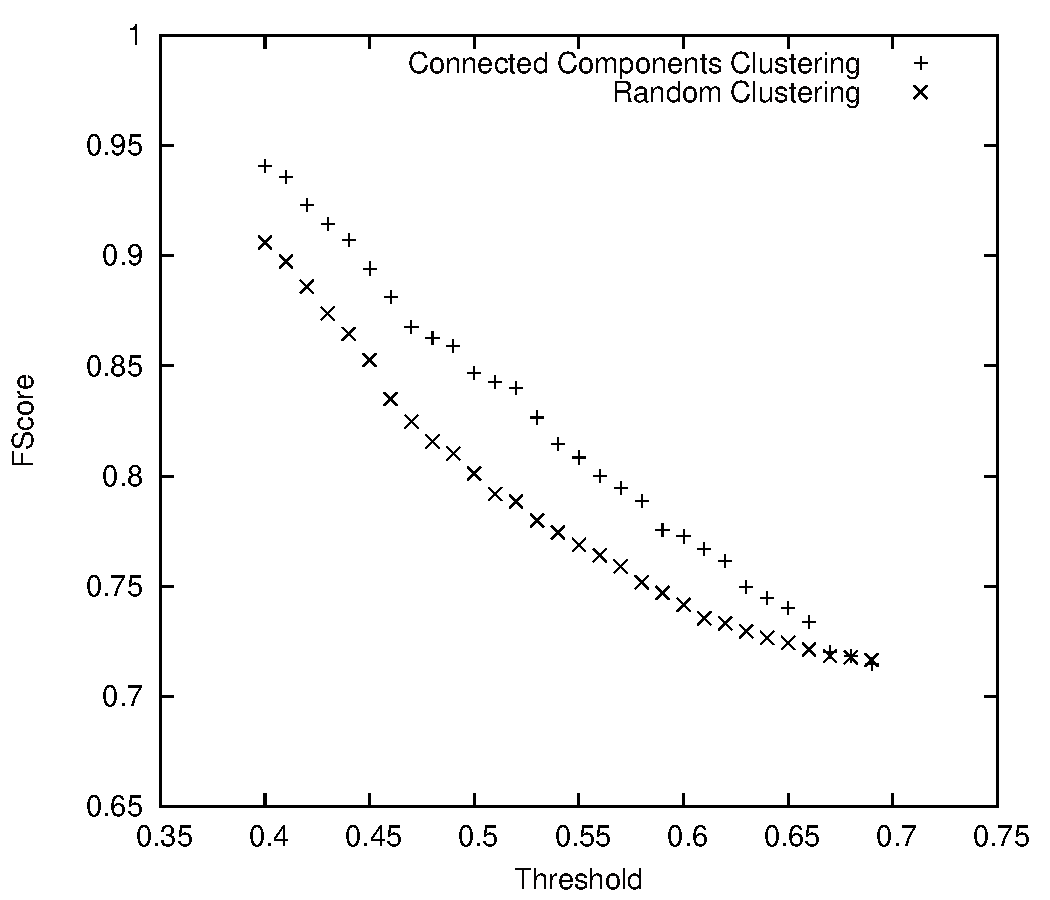
\includegraphics[width=2.9in]{SVMScaledSupervised7.pdf}\label{supervisedb}}
\subfigure[]{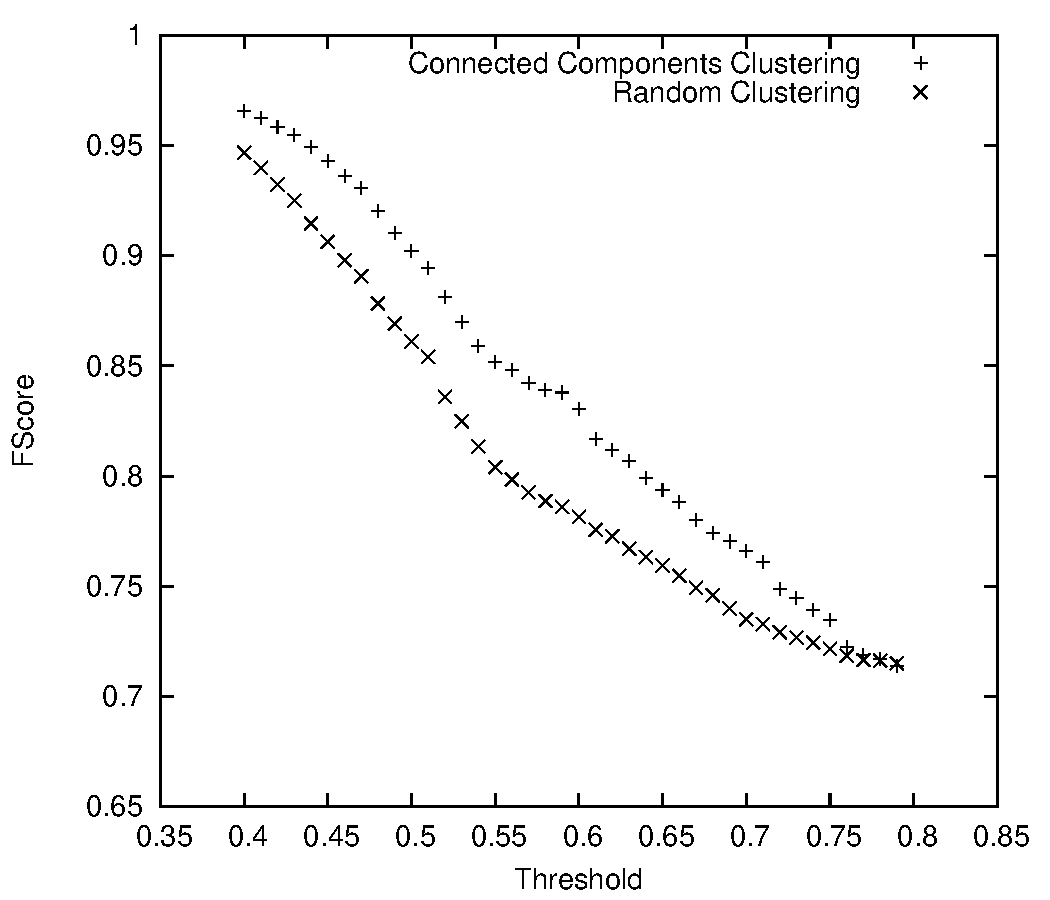
\includegraphics[width=2.9in]{SVMScaledSupervised8.pdf}\label{supervisedc}}
\caption{Improvement in average performance of best 3 Supervised Systems in Senseval-3 using Connected Component Clustering Vs Random Clustering at the same granularity with C = (a) 0.6, (b) 0.7 and (c) 0.8}
\label{fig:supervisedSystemsImprovement}
\end{figure}

\begin{figure}
\centering
\subfigure[]{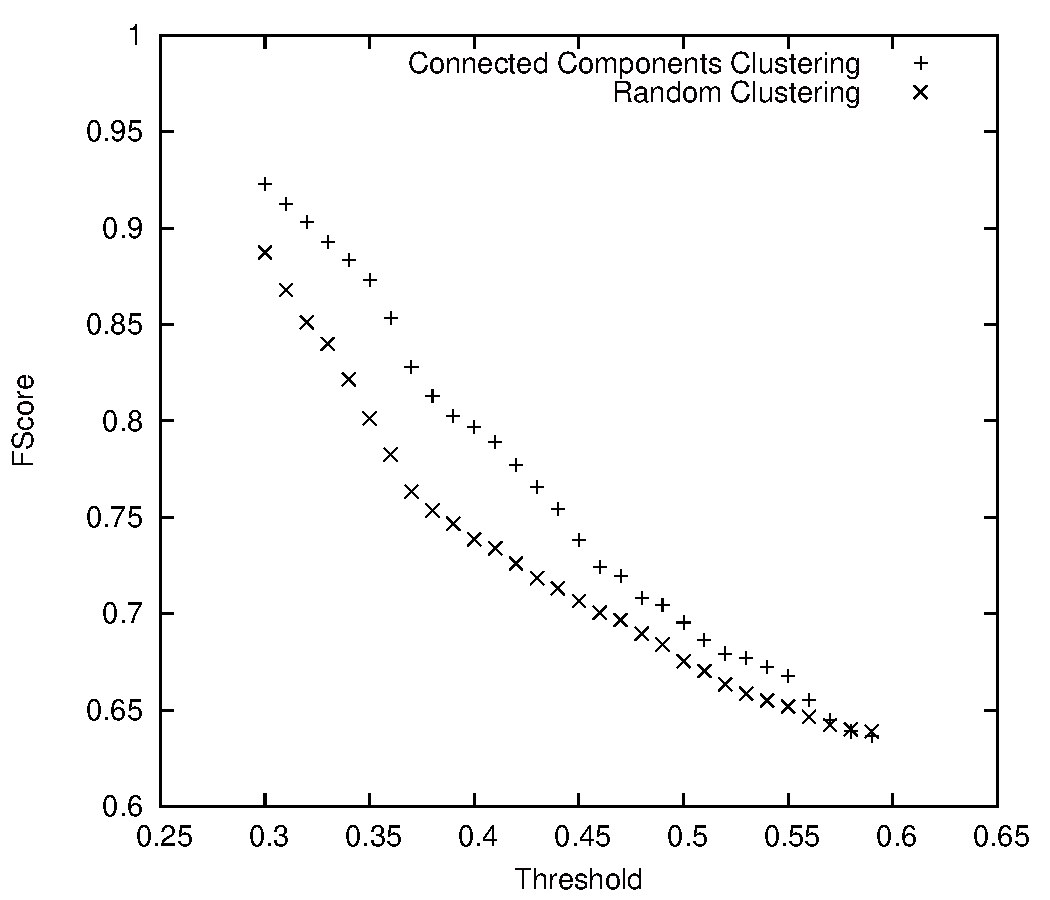
\includegraphics[width=2.9in]{SVMScaledUnsupervised6.pdf}\label{unsuperviseda}}
\subfigure[]{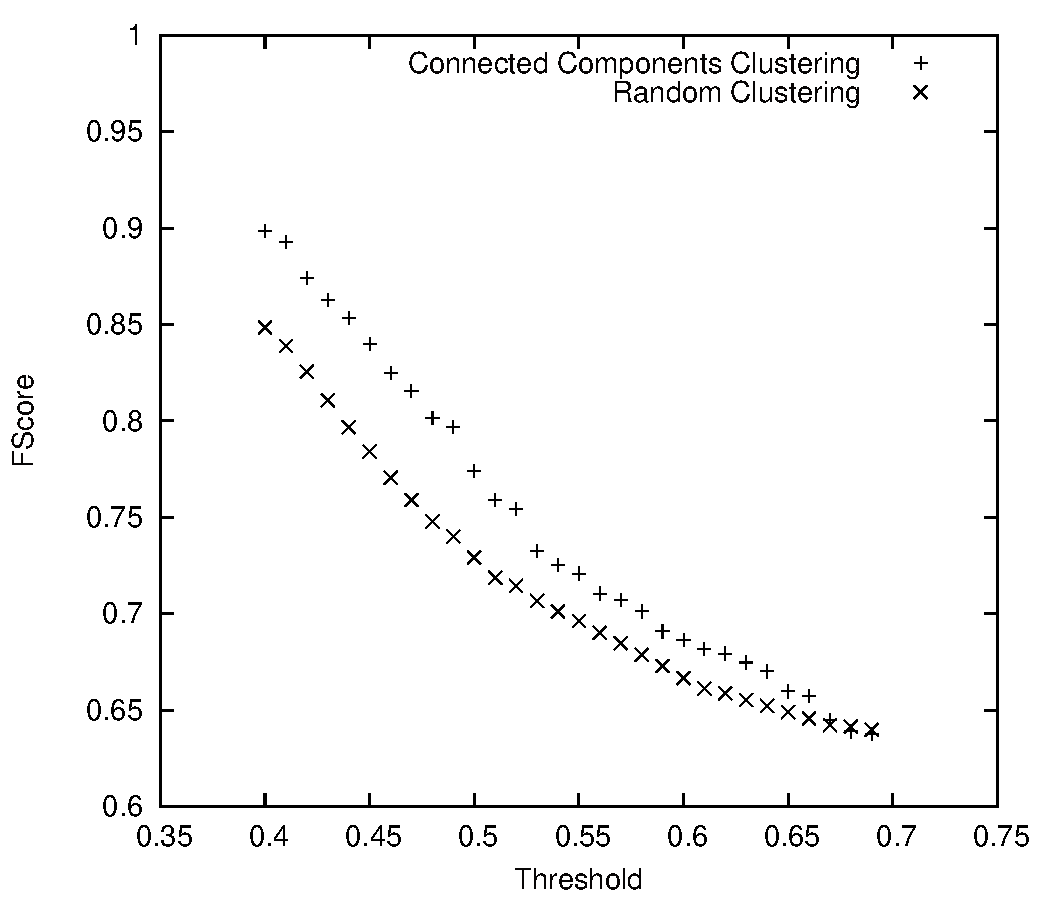
\includegraphics[width=2.9in]{SVMScaledUnsupervised7.pdf}\label{unsupervisedb}}
\subfigure[]{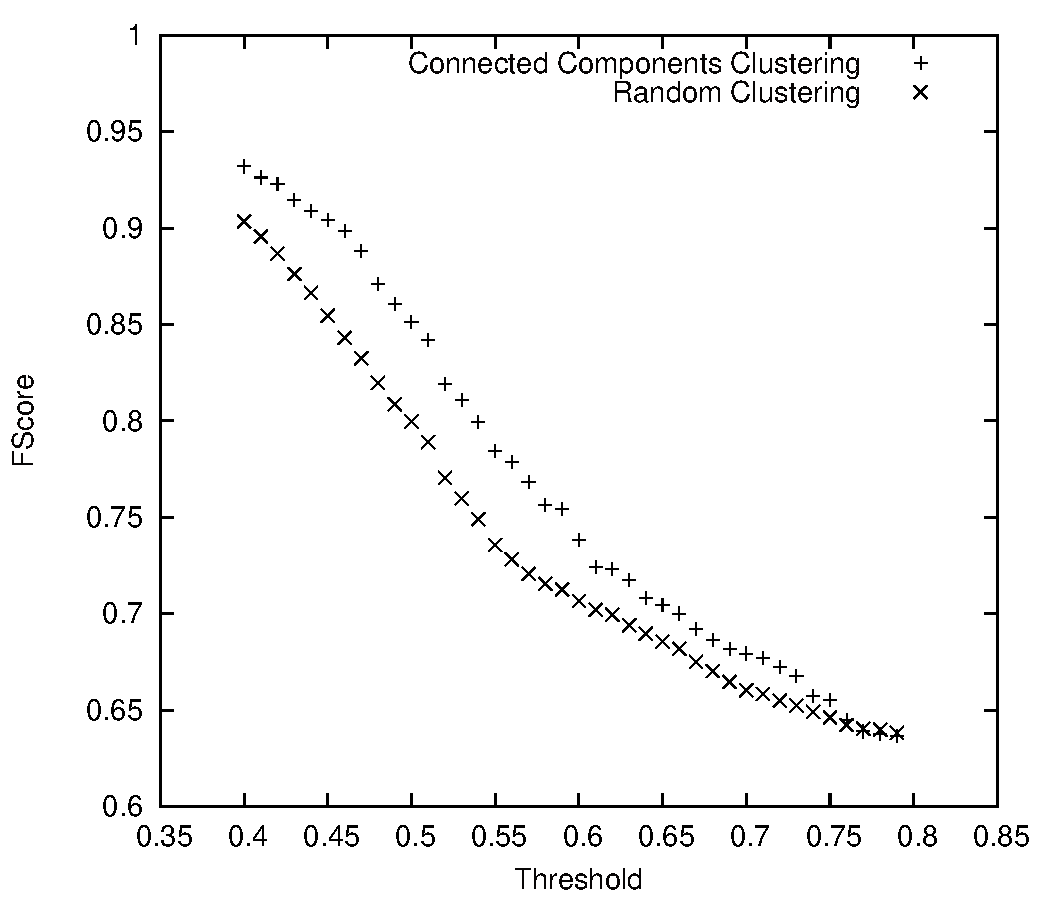
\includegraphics[width=2.9in]{SVMScaledUnsupervised8.pdf}\label{unsupervisedc}}
\caption{Improvement in performance of best Unupervised System in Senseval-3 using Connected Component Clustering Vs Random Clustering at the same granularity with C = (a) 0.6, (b) 0.7 and (c) 0.8}
\label{fig:unsupervisedSystemsImprovement}
\end{figure}

\section{Conclusions and Future Work}

\subsection{Conclusions}
The method discussed in the chapter learns a model for calculating synset similarity utilizing the taxonomy information and information learnt from manually obtained sense clustering. The framework obtained is generic and can be applied to other parts of speech as well.

For coarsening senses, we proposed one of the simplest approaches to cluster senses but it can be made to work with any clustering algorithm to generate coarse senses. We show that the clustering obtained by partitioning synsets in  connected components gives us a maximum improvement of 5.78\% on supervised systems and 7.18\% on unsupervised system.

\subsection{Future Work}

\subsubsection{Differentiating WordNet relations}
We use the WordNet relations \textit{Hypernymy}, \textit{Hyponymy}, \textit{Meronymy} and \textit{Holonymy} without any differentiation i.e. weights of all the links are unity. If we can grade the weights of the relations based on their relative importances, we can expect an improvement in the system. One way can be to perform cognitive experiments and obtain the weights of relations from the feedback of the annotators. An alternative way can be learn weights in a task based setting using an approach similar to \citep{Navigli05SSI}.

\subsubsection{Speeding up the implementation}
We used the naive implementation of SimRank, proposed in \citep{Jeh02simrank}, for implementing Personalized SimRank. Faster approximate scalable implementations of SimRank like \citep{FogarasSimRank}, \citep{LizorkinSimrank} etc. can also be adapted appropriately for personalization and thus speed up the algorithm.

                
    %    \chapter{Conclusions and Future Work}
\label{chapter:conclusion}
We presented an unsupervised neural network model that jointly learns fixed-length low-dimensional distributed vector representations for documents and words that encode the semantic content of the documents and words for multi-label document categorization. 
We overcome some of the issues in the bag-of-words representations by encoding the contextual information surrounding the words in the documents in our representations to improve their quality and performance on the categorization task.
Our neural network architecture is a linear-model that uses Noise Contrastive Estimation (NCE) to approximate the word probability distribution making parameter learning computationally inexpensive. We use the Stochastic Gradient Descent (SGD) to minimize the training objective that allows parallelization of the learning task further decreasing training time many folds.

We use a modified version of the logistic regression algorithm that learns distributed category representations by embedding categories in the same low-dimensional space as the documents and words for the multi-label document categorization task. 
On the standard \emph{Reuters-21578} dataset we show that using representations learned using model we achieve a F1 score of $91.7\%$ improving the bag-of-words representation accuracy by $9.03\%$ and the previous state-of-the-art, Multi-Class Maximum Figure-of-Merit (MC-MFoM) by $3.26\%$ in terms of the F1 score. 
We also present evaluations on the Wikipedia datasets showing that our representations perform better than the bag-of-words representations. We also show our model performs better than the bag-of-words representation at the task of imputing missing categories for existing articles on Wikipedia.
Using continuous vector representations we embed documents, words and categories in the same semantic space allowing us to estimate similarities between indirectly related entities such as words and categories. We qualitatively show that representations learned using our model capture the semantic similarity between categories and words effectively.

\section{Future Work}

\subsection{Include Syntactic Dependencies}

\subsection{Complex Learning Algos}

\subsection{Multi-view Joint Learning}
    %    \appendix
    %    \appendixpage
    %    \addappheadtotoc
    %   \chapter{Lexicographer Files}
\label{appendix:lexicographerFiles}
The names of the lexicographer files and their corresponding file numbers are listed below along with a brief description each file's contents. The table is reproduced from the WordNet manual \footnote{\url{http://wordnet.princeton.edu/man/lexnames.5WN.html}}.
\begin{center}
\begin{longtable}{|l|c|p{7cm}|}
\hline
File Number & Name & Contents \\ \hline
00 & adj.all & all adjective clusters \\ \hline
01 & adj.pert & relational adjectives (pertainyms) \\ \hline
02 & adv.all & all adverbs\\ \hline
03 & noun.Tops & unique beginner for nouns\\ \hline
04 & noun.act & nouns denoting acts or actions\\ \hline
05 & noun.animal & nouns denoting animals\\ \hline
06 & noun.artifact & nouns denoting man-made objects\\ \hline
07 & noun.attribute & nouns denoting attributes of people and objects\\ \hline
08 & noun.body & nouns denoting body parts\\ \hline
09 & noun.cognition & nouns denoting cognitive processes and contents\\ \hline
10 & noun.communication & nouns denoting communicative processes and contents\\ \hline
11 & noun.event & nouns denoting natural events\\ \hline
12 & noun.feeling & nouns denoting feelings and emotions\\ \hline
13 & noun.food & nouns denoting foods and drinks\\ \hline
14 & noun.group & nouns denoting groupings of people or objects\\ \hline
15 & noun.location & nouns denoting spatial position\\ \hline
16 & noun.motive & nouns denoting goals\\ \hline
17 & noun.object & nouns denoting natural objects (not man-made)\\ \hline
18 & noun.person & nouns denoting people\\ \hline
19 & noun.phenomenon & nouns denoting natural phenomena\\ \hline
20 & noun.plant & nouns denoting plants\\ \hline
21 & noun.possession & nouns denoting possession and transfer of possession\\ \hline
22 & noun.process & nouns denoting natural processes\\ \hline
23 & noun.quantity & nouns denoting quantities and units of measure\\ \hline
24 & noun.relation & nouns denoting relations between people or things or ideas\\ \hline
25 & noun.shape	nouns & denoting two and three dimensional shapes\\ \hline
26 & noun.state	nouns & denoting stable states of affairs\\ \hline
27 & noun.substance & nouns denoting substances\\ \hline
28 & noun.time & nouns denoting time and temporal relations\\ \hline
29 & verb.body & verbs of grooming, dressing and bodily care\\ \hline
30 & verb.change & verbs of size, temperature change, intensifying, etc.\\ \hline
31 & verb.cognition & verbs of thinking, judging, analyzing, doubting\\ \hline
32 & verb.communication & verbs of telling, asking, ordering, singing\\ \hline
33 & verb.competition & verbs of fighting, athletic activities\\ \hline
34 & verb.consumption & verbs of eating and drinking\\ \hline
35 & verb.contact & verbs of touching, hitting, tying, digging\\ \hline
36 & verb.creation & verbs of sewing, baking, painting, performing\\ \hline
37 & verb.emotion & verbs of feeling\\ \hline
38 & verb.motion & verbs of walking, flying, swimming\\ \hline
39 & verb.perception & verbs of seeing, hearing, feeling\\ \hline
40 & verb.possession & verbs of buying, selling, owning\\ \hline
41 & verb.social & verbs of political and social activities and events\\ \hline
42 & verb.stative & verbs of being, having, spatial relations\\ \hline
43 & verb.weather & verbs of raining, snowing, thawing, thundering\\ \hline
44 & adj.ppl & participial adjectives\\ \hline
\caption{Lexicographer Files and Description} % needs to go inside longtable environment
\label{tab:lexicographerFiles}
\end{longtable}
\end{center}





















    %    \chapter{Results for SVM Experiments}
\label{appendix:SVMResults}

The appendix jots down the performance of the SVMs learnt on random datasets as described in section \ref{section:SVMNormalizationKernelExperiment}.
The performance criteria are Precision, Recall, FScore (on both Positive and Negative classes) and Accuracy.

\begin{center}
\begin{longtable}{| c | c | c | c | c | c |}      
    \hline
    Performance Measure & Dataset 1 & Dataset 2 & Dataset 3 & Dataset 4 & Dataset 5 \\ \hline
    Accuracy & 0.5687 & 0.5769 & 0.5646 & 0.5755 & 0.5467 \\ \hline 
    PrecisionP & 0.7404 & 0.75 & 0.7117 & 0.7570 & 0.8542 \\ \hline
    RecallP & 0.2115 & 0.2308 & 0.2170 & 0.2225 & 0.1126 \\ \hline
    FScoreP & 0.3291 & 0.3529 & 0.3326 & 0.3439 & 0.1990 \\ \hline % 0.3115
    PrecisionN & 0.5401 & 0.5454 & 0.5381 & 0.5443 & 0.525 \\ \hline
    RecallN & 0.9258 & 0.9231 & 0.9121 & 0.9286 & 0.9808 \\ \hline
    FScoreN & 0.6822 & 0.6857 & 0.6769 & 0.6863 & 0.6839 \\ \hline % 0.6830
    \caption{Linear Kernel - No Normalization}
  \label{tab:LinearKernelNoNormalization}
\end{longtable}
\end{center}

\begin{center}
\begin{longtable}{| c | c | c | c | c | c |}      
    \hline
    Performance Measure & Dataset 1 & Dataset 2 & Dataset 3 & Dataset 4 & Dataset 5 \\ \hline
    Accuracy & 0.7019 & 0.7376 & 0.7253 & 0.7294 & 0.7198 \\ \hline
    PrecisionP & 0.6889 & 0.7357 & 0.7265 & 0.7158 & 0.7222 \\ \hline
    RecallP & 0.7363 & 0.7418 & 0.7225 & 0.7610 & 0.7143 \\ \hline
    FScoreP & 0.7118 & 0.7387 & 0.7245 & 0.7377 & 0.7182 \\ \hline % 0.72618
    PrecisionN & 0.7168 & 0.7396 & 0.7240 & 0.7449 & 0.7174 \\ \hline
    RecallN & 0.6676 & 0.7335 & 0.7280 & 0.6978 & 0.7253 \\ \hline
    FScoreN & 0.6913 & 0.7366 & 0.7260 & 0.7206 & 0.7213 \\ \hline % 0.71916
    \caption{Linear Kernel - MinMax Normalization}
  \label{tab:LinearKernelMinMaxNormalization}
\end{longtable}
\end{center}

\begin{center}
\begin{longtable}{| c | c | c | c | c | c |}      
    \hline
    Performance Measure & Dataset 1 & Dataset 2 & Dataset 3 & Dataset 4 & Dataset 5 \\ \hline
    Accuracy & 0.5096 & 0.5151 & 0.5027 & 0.5069 & 0.5192 \\ \hline 
    PrecisionP & 0.7333 & 0.9231 & 0.75 & 1.0 & 0.9375 \\ \hline
    RecallP & 0.03022 & 0.0330 & 0.0082 & 0.0137 & 0.0412 \\ \hline
    FScoreP & 0.05805 & 0.0637 & 0.0163 & 0.0271 & 0.0789 \\ \hline % 0.04881
    PrecisionN & 0.5049 & 0.5077 & 0.5014 & 0.5035 & 0.5098 \\ \hline
    RecallN & 0.9890 & 0.9972 & 0.9972 & 1.0 & 0.9972 \\ \hline
    FScoreN & 0.6685 & 0.6728 & 0.6673 & 0.6697 & 0.6747 \\ \hline % 0.6706
    \caption{Linear Kernel - ZScore Normalization}
  \label{tab:LinearKernelZScoreNormalization}
\end{longtable}
\end{center}

\begin{center}
\begin{longtable}{| c | c | c | c | c | c |}      
    \hline
    Performance Measure & Dataset 1 & Dataset 2 & Dataset 3 & Dataset 4 & Dataset 5 \\ \hline
    Accuracy & 0.6003 & 0.6058 & 0.5797 & 0.5948 & 0.5934 \\ \hline
    PrecisionP & 0.5588 & 0.5626 & 0.5459 & 0.5554 & 0.5556 \\ \hline
    RecallP & 0.9533 & 0.9505 & 0.9478 & 0.9505 & 0.9341 \\ \hline
    FScoreP & 0.7046 & 0.7068 & 0.6928 & 0.7011 & 0.6967 \\ \hline % 0.7004
    PrecisionN & 0.8411 & 0.8407 & 0.8021 & 0.8286 & 0.7931 \\ \hline
    RecallN & 0.2472 & 0.2610 & 0.2115 & 0.2390 & 0.2527 \\ \hline
    FScoreN & 0.3822 & 0.3983 & 0.3348 & 0.3710 & 0.3833 \\ \hline % 0.37392
    \caption{RBF Kernel - No Normalization}
  \label{tab:RBFKernelNoNormalization}
\end{longtable}
\end{center}

\begin{center}
\begin{longtable}{| c | c | c | c | c | c |}      
    \hline
    Performance Measure & Dataset 1 & Dataset 2 & Dataset 3 & Dataset 4 & Dataset 5 \\ \hline
    Accuracy & 0.7212 & 0.7198 & 0.7184 & 0.7308 & 0.7033  \\ \hline
    PrecisionP & 0.7007 & 0.7083 & 0.6897 & 0.6972 & 0.6787  \\ \hline
    RecallP & 0.7720 & 0.7472 & 0.7939 & 0.8159 & 0.7720  \\ \hline
    FScoreP & 0.7346 & 0.7273 & 0.7382 & 0.7519 & 0.7224  \\ \hline % 0.73488
    PrecisionN & 0.7462 & 0.7326 & 0.7573 & 0.7781 & 0.7357  \\ \hline
    RecallN & 0.6703 & 0.6923 & 0.6428 & 0.6456 & 0.6346  \\ \hline
    FScoreN & 0.7062 & 0.7119 & 0.6954 & 0.7057 & 0.6814  \\ \hline % 0.70012
    \caption{RBF Kernel - MinMax Normalization}
  \label{tab:RBFKernelMinMaxNormalization}
\end{longtable}
\end{center}


\begin{center}
\begin{longtable}{| c | c | c | c | c | c |}      
    \hline
    Performance Measure & Dataset 1 & Dataset 2 & Dataset 3 & Dataset 4 & Dataset 5 \\ \hline
    Accuracy & 0.6731 & 0.6992 & 0.6648 & 0.6882 & 0.6799  \\ \hline 
    PrecisionP & 0.7316 & 0.7757 & 0.7325 & 0.7354 & 0.7347  \\ \hline
    RecallP & 0.5467 & 0.5604 & 0.5192 & 0.5879 & 0.5632  \\ \hline
    FScoreP & 0.6258 & 0.6507 & 0.6077 & 0.6534 & 0.6376  \\ \hline % 0.63504
    PrecisionN & 0.6382 & 0.6559 & 0.6276 & 0.6568 & 0.6459  \\ \hline
    RecallN & 0.7994 & 0.8379 & 0.8104 & 0.7885 & 0.7967  \\ \hline
    FScoreN & 0.7097 & 0.7358 & 0.7074 & 0.7166 & 0.7134  \\ \hline % 0.71658
    \caption{RBF Kernel - ZScore Normalization}
  \label{tab:RBFKernelZScoreNormalization}
\end{longtable}
\end{center}


    %    \chapter{Weighted SimRank}
\label{appendix:weightedSimRank}
We discuss the weighted SimRank Model here along with the theoretical interpretation using Random Surfer-Pairs Model.

\section{Random Surfer-Pairs Model}
We extend the Random Surfer-Pairs Model and Expected-f Meeting Distance discussed in \citep{Jeh02simrank} to a weighted graph.
We define $s'(\alpha,\beta)$, the similarity between $\alpha$ and $\beta$ in $G$ based on \textit{expected-f meeting distance}, with $f(z) = c^z$, as

\begin{equation}
s'(a,b) = \sum_{t:(a,b) \rightsquigarrow (x,x)} P[t]c^{l(t)}  \label{eq:emdWeighted} 
\end{equation}

where $c$ is the a positive constant less than 1. 
If there is no tour from $(\alpha,\beta)$ to any singleton node, the summation is taken to be $0$. 
Note from equation \ref{eq:emdWeighted} that $s'(\alpha,\beta) \in [0, 1]$ for all $\alpha,\beta$, and that $s'(\alpha,\beta) = 1$ if $\alpha=\beta$.

\section{Equivalence}
For presentation ease, let us assume that all edges in the graph G have been reversed. So following an edge in the reversed graph is same as moving one step backwards in the original graph.

We compute the expected-f meeting distance on lines of computation of expected distance in the graph.
Suppose a surfer is at $u \in V$. 
In the next step, he chooses one of $O_1(u), \ldots, O_{|O(u)|}(u)$, say $O_i(u)$, proportional with the corresponding edge weight i.e. with probability $\frac{w(u,O_i(u))}{W_O(u)}$.
On choosing $O_i(u)$, the process is repeated.

We'll now show that $s'(\alpha,\beta) = s(\alpha,\beta)$

\begin{align}
s'(\alpha,\beta)  
 &= \sum_{z=1}^{|O((\alpha,\beta))|} \sum_{t':O_z((\alpha,\beta)) \rightsquigarrow (x,x)} P[(\alpha,\beta) \rightarrow O_z(\alpha,\beta) \overset{t'}{\rightsquigarrow} (x,x)]  \cdot  c^{l(t')+1}  \notag \\
 &= c \sum_{z=1}^{|O((\alpha,\beta))|} \sum_{t':O_z((\alpha,\beta)) \rightsquigarrow (x,x)} P((\alpha,\beta) \rightarrow O_z(\alpha,\beta))  \cdot  P[t']  \cdot  c^{l(t')}    \notag \\
 &= c \sum_{z=1}^{|O((\alpha,\beta))|} P((\alpha,\beta) \rightarrow O_z(\alpha,\beta))  \sum_{t':O_z((\alpha,\beta)) \rightsquigarrow (x,x)}   P[t']  \cdot  c^{l(t')}    \notag \\
 &= c \sum_{z=1}^{|O((\alpha,\beta))|} P((\alpha,\beta) \rightarrow O_z(\alpha,\beta))  \cdot s'(O_z(\alpha,\beta))    \notag \\
 &= c \sum_{i=1}^{|O(\alpha)|} \sum_{j=1}^{|O(\beta)|} P((\alpha,\beta) \rightarrow (O_i(\alpha),O_j(\beta)))  \cdot s'(O_i(\alpha),O_j(\beta))    \notag \\
 &= c \sum_{i=1}^{|O(\alpha)|} \sum_{j=1}^{|O(\beta)|} \frac{ w(\alpha,O_i(\alpha)) \cdot w(\beta,O_j(\beta)) } { W_{O}(\alpha) \cdot W_O(\beta)}  \cdot s'(O_i(\alpha),O_j(\beta))    \notag \\
 &= \frac{c}{{ W_{O}(\alpha) \cdot W_O(\beta)}} \sum_{i=1}^{|O(\alpha)|} \sum_{j=1}^{|O(\beta)|} w(\alpha,O_i(\alpha)) \cdot w(\beta,O_j(\beta)) \cdot s'(O_i(\alpha),O_j(\beta)) \label{eq:SimRankWeightedReversed}
\end{align}

Equation \ref{eq:SimRankWeightedReversed} is identical to the SimRank equation \ref{eq:SimRankWeighted} with $c = C$ and in-edges swapped for out-edges. 
Since the solution to \ref{eq:SimRankWeighted} is unique\footnote{Straight forward proof on lines of SimRank. Refer \citep{Jeh02simrank}}, $s'(\alpha, \beta) = s(\alpha, \beta)$ for all $\alpha, \beta \in V$ . 
    %    \chapter{Personalized SimRank Properties}
\label{appendix:PersonalizedSimRankProperties}

In this appendix, we prove some of the important properties of the Personalized SimRank System introduced in Section \ref{subsection:PersonalizedSimRank}.\\

\noindent
\textsc{Proposition 0} : The sequence $S_k(\alpha,\beta)$ converges for every node pair $\alpha,\beta \in V$

\noindent
\textsc{Proof} :
It follows from the monotonocity of the sequence $S_k(\alpha,\beta)$ : 
\begin{equation}
0 \leq S_k(\alpha,\beta) \leq S_{k+1}(\alpha,\beta) \leq 1 \mbox{ for all } \alpha,\beta \in V, k \geq 0
\end{equation}

This says for every $\alpha,\beta$, the sequence $\{S_k(\alpha,\beta)\}$ is bounded and non-decreasing as $k$ increases and hence each sequence $\{S_k(\alpha,\beta)\}$ converges to a limit $S(\alpha,\beta) \in [0,1]$.\\

\noindent
\textsc{Proposition 1} : The system of equations of Personalized SimRank has a solution, which is constructed by the iterative fixed point solution defined in Section \ref{subsection:PersonalizedSimRank}.

\noindent
\textsc{Proof} :
The unique solution is actually constructed in Section \ref{subsection:PersonalizedSimRank}, and the correctness of the iterative algorithm follows. 

Using \textsc{Proposition 0} and the fact that limit of a sum is the sum of the limits, we have :
\begin{equation} \label{eq:PersonalizedWeightedSimRankLimit}
{\footnotesize
S(\alpha,\beta) =
\left\{ \begin{array}{rl}
1 & \mbox{if } \alpha=\beta\\
InitStore[(\alpha,\beta)] & \mbox{if } (\alpha,\beta) \in InitStore\\
\frac{C}{W_{I}(\alpha)W_{I}(\beta)} \sum_{i=1}^{|I(\alpha)|} \sum_{j=1}^{|I(\beta)|} w(I_i(\alpha),\alpha) \cdot w(I_j(\beta),\beta) \cdot S(I_i(\alpha),I_j(\beta)) & \mbox{otherwise }
\end{array}\right.
}
\end{equation}

which shows that the limits $S(\ast, \ast)$ satisfy the simrank equations. \\

\noindent
\textsc{Proposition 2} : The system of equations of Personalized SimRank has a unique solution.

\noindent
\textsc{Proof} :
Suppose $s_1(\ast,\ast)$ and $s_2(\ast,\ast)$ are two solutions to the $|V|^2$ Personalized SimRank equations.
For all $\alpha,\beta \in V$, let $\delta(\alpha,\beta) = s_1(\alpha,\beta)-s_2(\alpha,\beta)$ be their difference. 
Let $M = max_{(\alpha,\beta)}|\delta(\alpha,\beta)|$ be the maximum absolute value of any difference.
We need to show that $M=0$.
Let $|\delta(\alpha,\beta)| = M$ for some $\alpha,\beta \in V$. Certainly $M=0$ if $\alpha,\beta$ or if $(\alpha,\beta)\in InitStore$ or if $I(\alpha) = \emptyset$ or $I(\beta)=\emptyset$.
Otherwise, $s_1(\alpha,\beta)$ and $s_2(\alpha,\beta)$ are the weighted average scores of their in-neighbours. 
That is, from equation \ref{eq:PersonalizedWeightedSimRank},

\begin{align*}
s_1(\alpha,\beta) =& \frac{C}{W_{I}(\alpha)W_{I}(\beta)} \sum_{i=1}^{|I(\alpha)|} \sum_{j=1}^{|I(\beta)|} w(I_i(\alpha),\alpha) \cdot w(I_j(\beta),\beta) \cdot s_1(I_i(\alpha),I_j(\beta))\\
s_2(\alpha,\beta) =& \frac{C}{W_{I}(\alpha)W_{I}(\beta)} \sum_{i=1}^{|I(\alpha)|} \sum_{j=1}^{|I(\beta)|} w(I_i(\alpha),\alpha) \cdot w(I_j(\beta),\beta) \cdot s_2(I_i(\alpha),I_j(\beta))\\
\end{align*}

\noindent
In terms of $\delta(\alpha,\beta)$,
\begin{align*}
\delta(\alpha,\beta) =& s_1(\alpha,\beta) - s_2(\alpha,\beta)\\
=& \frac{C}{W_{I}(\alpha)W_{I}(\beta)} \sum_{i=1}^{|I(\alpha)|} \sum_{j=1}^{|I(\beta)|} w(I_i(\alpha),\alpha) \cdot w(I_j(\beta),\beta) \cdot [s_1(I_i(\alpha),I_j(\beta)) - s_2(I_i(\alpha),I_j(\beta))]\\
=&\frac{C}{W_{I}(\alpha)W_{I}(\beta)} \sum_{i=1}^{|I(\alpha)|} \sum_{j=1}^{|I(\beta)|} w(I_i(\alpha),\alpha) \cdot w(I_j(\beta),\beta) \cdot \delta(I_i(\alpha),I_j(\beta))
\end{align*}

\noindent
Thus, 
\begin{align*}
M =& |\delta(\alpha,\beta)|\\
=& \left| \frac{C}{W_{I}(\alpha)W_{I}(\beta)} \sum_{i=1}^{|I(\alpha)|} \sum_{j=1}^{|I(\beta)|} w(I_i(\alpha),\alpha) \cdot w(I_j(\beta),\beta) \cdot \delta(I_i(\alpha),I_j(\beta))\right|\\
\leq& \frac{C}{W_{I}(\alpha)W_{I}(\beta)} \sum_{i=1}^{|I(\alpha)|} \sum_{j=1}^{|I(\beta)|} w(I_i(\alpha),\alpha) \cdot w(I_j(\beta),\beta) \cdot \left| \delta(I_i(\alpha),I_j(\beta))\right|\\
\leq&\frac{C}{W_{I}(\alpha)W_{I}(\beta)} \sum_{i=1}^{|I(\alpha)|} \sum_{j=1}^{|I(\beta)|} w(I_i(\alpha),\alpha) \cdot w(I_j(\beta),\beta) \cdot M\\
=& CM
\end{align*}

\noindent
Since $0 < C < 1$, it follows that $M=0$\\

\noindent
\textsc{Proposition 3} : \textit{The difference between SimRank theoretical and iterative similarity scores decreases exponentially in the number of iterations for every pair of nodes. 
Precisely, for every iteration number $t = 0, 1, 2, \ldots$ and for every two nodes $\alpha,\beta$, the following estimate holds:}
\begin{align}
s(\alpha,\beta) - S_{t}(\alpha,\beta) \leq C^{t+1} \label{eq:convergenceSimRankPersonalized}
\end{align}

\noindent
\textsc{Proof} :
If $\alpha=\beta$ then $s(\alpha,\alpha)=S_k(\alpha,\alpha)=1$ by definition for every $k=0,1,2,\ldots$, the left side of \ref{eq:convergenceSimRankPersonalized} is 0 and thus \ref{eq:convergenceSimRankPersonalized} obviously holds.
Similarly, if $I(\alpha) = \emptyset$ or $I(\beta) = \emptyset$ then by definition $s(\alpha,\beta)=S_k(\alpha,\beta)=0$.
Also, lets consider the case when $(\alpha,\beta)\in InitStore$. In this case, $s(\alpha,\beta)=S_k(\alpha,\beta)=InitStore[(\alpha,\beta)]$ and hence \ref{eq:convergenceSimRankPersonalized} always holds.

For the general case of $\alpha \neq \beta$, $I(\alpha) \neq \emptyset$, $I(\beta) \neq \emptyset$ and $(\alpha,\beta) \in InitStore$, the proof is organized by mathematical induction.

\textbf{Induction Basis} : Let us prove that \ref{eq:convergenceSimRankPersonalized} holds for $k=0$ i.e. for every two nodes $\alpha,\beta$ :
\begin{align}
s(\alpha,\beta) - S_0(\alpha,\beta) \leq C \label{eq:baseCase}
\end{align}

Since $\alpha \neq \beta$, $I(\alpha) \neq \emptyset$, $I(\beta) \neq \emptyset$ and $(\alpha,\beta) \in InitStore$, then $S_0(\alpha,\beta)=0$. 
\begin{align*}
s(\alpha,\beta) - S_0(\alpha,\beta) &= s(\alpha,\beta)\\
&=\frac{C}{W_{I}(\alpha)W_{I}(\beta)} \sum_{i=1}^{|I(\alpha|} \sum_{j=1}^{|I(\beta)|} w(I_i(\alpha),\alpha) \cdot w(I_j(\beta),\beta) \cdot \underbrace{s(I_i(\alpha),I_j(\beta))}_{\leq 1}\\
&=\frac{C}{W_{I}(\alpha)W_{I}(\beta)} \sum_{i=1}^{|I(a)|} \sum_{j=1}^{|I(\beta)|} w(I_i(\alpha),\alpha) \cdot w(I_j(\beta),\beta) \\
&\leq C
\end{align*}
which proves \ref{eq:baseCase}

\textbf{Inductive Step} : Provided that \ref{eq:convergenceSimRankPersonalized} holds for a given $k$ for all node pairs, let us prove that \ref{eq:convergenceSimRankPersonalized} holds for $(k+1)$ as well:
\begin{align*}
s(\alpha,\beta) - S_{k+1}(\alpha,\beta) &= \frac{C}{W_{I}(\alpha)W_{I}(\beta)} \sum_{i=1}^{|I(\alpha)|} \sum_{j=1}^{|I(\beta)|} w(I_i(\alpha),\alpha) \cdot w(I_j(\beta),\beta) \cdot s(I_i(\alpha),I_j(\beta))\\
&-\frac{C}{W_{I}(\alpha)W_{I}(\beta)} \sum_{i=1}^{|I(\alpha)|} \sum_{j=1}^{|I(\beta)|} w(I_i(\alpha),\alpha) \cdot w(I_j(\beta),\beta) \cdot S_k(I_i(\alpha),I_j(\beta)) \\
&=\frac{C}{W_{I}(\alpha)W_{I}(\beta)}\\
&\sum_{i=1}^{|I(\alpha)|} \sum_{j=1}^{|I(\beta)|} w(I_i(\alpha),\alpha) \cdot w(I_j(\beta),\beta) \cdot \underbrace{[s(I_i(\alpha),I_j(\beta))-S_k(I_i(\alpha),I_j(\beta))]}_{\leq C^{k+1} \mbox{ by inductive hypothesis}}\\
&\leq C^{(k+1)+1}
\end{align*}

The latter finally proves \ref{eq:convergenceSimRankPersonalized}.



    %    \chapter{Probabilistic Outputs for SVM}
\label{appendix:SVMProb}
The following is the improved code by \citep{Lin03Note} for the algorithm proposed originally by \citep{Platt99}, that theoretically converges and avoids numerical difficulties.

\begin{verbatim}

Input parameters:
  deci = array of SVM decision values
  label = array of booleans: is the example labeled +1?
  prior1 = number of positive examples
  prior0 = number of negative examples
Outputs:
  A, B = parameters of sigmoid
  
//Parameter setting
maxiter=100
//Maximum number of iterations
minstep=1e-10
//Minimum step taken in line search
sigma=1e-12
//Set to any value > 0
//Construct initial values: target support in array t,
//initial function value in fval
hiTarget=(prior1+1.0)/(prior1+2.0), loTarget=1/(prior0+2.0)
len=prior1+prior0 // Total number of data
for i = 1 to len {
    if (label[i] > 0)
        t[i]=hiTarget
    else
        t[i]=loTarget
}
A=0.0, B=log((prior0+1.0)/(prior1+1.0)), fval=0.0
for i = 1 to len {
    fApB=deci[i]*A+B
    if (fApB >= 0)
        fval += t[i]*fApB+log(1+exp(-fApB))
    else
        fval += (t[i]-1)*fApB+log(1+exp(fApB))
}
for it = 1 to maxiter {
    //Update Gradient and Hessian (use H’ = H + sigma I)
    h11=h22=sigma, h21=g1=g2=0.0
    for i = 1 to len {
        fApB=deci[i]*A+B
        if (fApB >= 0)
            p=exp(-fApB)/(1.0+exp(-fApB)), q=1.0/(1.0+exp(-fApB))
        else
            p=1.0/(1.0+exp(fApB)), q=exp(fApB)/(1.0+exp(fApB))
        d2=p*q
        h11 += deci[i]*deci[i]*d2, h22 += d2, h21 += deci[i]*d2
        d1=t[i]-p
        g1 += deci[i]*d1, g2 += d1
    }
    if (abs(g1)<1e-5 && abs(g2)<1e-5) //Stopping criteria
        break
    //Compute modified Newton directions
    det=h11*h22-h21*h21
    dA=-(h22*g1-h21*g2)/det, dB=-(-h21*g1+h11*g2)/det
    gd=g1*dA+g2*dB
    stepsize=1
    while (stepsize >= minstep){ //Line search
        newA=A+stepsize*dA, newB=B+stepsize*dB, newf=0.0
        for i = 1 to len {
            fApB=deci[i]*newA+newB
            if (fApB >= 0)
                newf += t[i]*fApB+log(1+exp(-fApB))
            else
                newf += (t[i]-1)*fApB+log(1+exp(fApB))
        }
        if (newf<fval+0.0001*stepsize*gd){
            A=newA, B=newB, fval=newf
            break //Sufficient decrease satisfied
        }
        else
            stepsize /= 2.0
    }
    if (stepsize < minstep){
        print ’Line search fails’
        break
    }
}
if (it >= maxiter)
    print ’Reaching maximum iterations’
return [A,B]
\end{verbatim}
                
	\backmatter
	\singlespacing
	\addcontentsline{toc}{chapter}{Bibliography}
	%\bibliographystyle{unsrt}
%       \bibliographystyle{alpha}
	\bibliographystyle{plainnat}
	\bibliography{references}

\end{document}
